\documentclass{book}
\usepackage[a4paper,top=2.5cm,bottom=2.5cm,left=2.5cm,right=2.5cm]{geometry}
\usepackage{makeidx}
\usepackage{natbib}
\usepackage{graphicx}
\usepackage{multicol}
\usepackage{float}
\usepackage{listings}
\usepackage{color}
\usepackage{ifthen}
\usepackage[table]{xcolor}
\usepackage{textcomp}
\usepackage{alltt}
\usepackage{ifpdf}
\ifpdf
\usepackage[pdftex,
            pagebackref=true,
            colorlinks=true,
            linkcolor=blue,
            unicode
           ]{hyperref}
\else
\usepackage[ps2pdf,
            pagebackref=true,
            colorlinks=true,
            linkcolor=blue,
            unicode
           ]{hyperref}
\usepackage{pspicture}
\fi
\usepackage[utf8]{inputenc}
\usepackage{mathptmx}
\usepackage[scaled=.90]{helvet}
\usepackage{courier}
\usepackage{sectsty}
\usepackage{amssymb}
\usepackage[titles]{tocloft}
\usepackage{doxygen}
\lstset{language=C++,inputencoding=utf8,basicstyle=\footnotesize,breaklines=true,breakatwhitespace=true,tabsize=8,numbers=left }
\makeindex
\setcounter{tocdepth}{3}
\renewcommand{\footrulewidth}{0.4pt}
\renewcommand{\familydefault}{\sfdefault}
\hfuzz=15pt
\setlength{\emergencystretch}{15pt}
\hbadness=750
\tolerance=750
\begin{document}
\hypersetup{pageanchor=false,citecolor=blue}
\begin{titlepage}
\vspace*{7cm}
\begin{center}
{\Large I\-O\-O\-O \mbox{[}ay-\/oo\mbox{]} Input/\-Output object oriented }\\
\vspace*{1cm}
{\large Generated by Doxygen 1.8.3.1}\\
\vspace*{0.5cm}
{\small Wed Jul 10 2013 01:25:43}\\
\end{center}
\end{titlepage}
\clearemptydoublepage
\pagenumbering{roman}
\tableofcontents
\clearemptydoublepage
\pagenumbering{arabic}
\hypersetup{pageanchor=true,citecolor=blue}
\chapter{Hierarchical Index}
\section{Class Hierarchy}
This inheritance list is sorted roughly, but not completely, alphabetically\-:\begin{DoxyCompactList}
\item \contentsline{section}{Beagle\-Goo\-:\-:G\-P\-I\-O\-Info}{\pageref{struct_beagle_goo_1_1_g_p_i_o_info}}{}
\item gpio\-Infos\begin{DoxyCompactList}
\item \contentsline{section}{Beagle\-Goo}{\pageref{struct_beagle_goo}}{}
\end{DoxyCompactList}
\item \contentsline{section}{G\-P\-I\-Ooo}{\pageref{class_g_p_i_ooo}}{}
\begin{DoxyCompactList}
\item \contentsline{section}{Beagle\-Goo}{\pageref{struct_beagle_goo}}{}
\end{DoxyCompactList}
\item \contentsline{section}{G\-P\-I\-Opin}{\pageref{class_g_p_i_opin}}{}
\begin{DoxyCompactList}
\item \contentsline{section}{Beagle\-Goo\-P}{\pageref{class_beagle_goo_p}}{}
\end{DoxyCompactList}
\item \contentsline{section}{H\-D44780}{\pageref{class_h_d44780}}{}
\item \contentsline{section}{H\-D44780phy}{\pageref{class_h_d44780phy}}{}
\begin{DoxyCompactList}
\item \contentsline{section}{H\-D44780gpio\-Phy}{\pageref{class_h_d44780gpio_phy}}{}
\end{DoxyCompactList}
\item \contentsline{section}{pru\-\_\-data}{\pageref{structpru__data}}{}
\item \contentsline{section}{S\-P\-I}{\pageref{class_s_p_i}}{}
\item \contentsline{section}{Test\-G\-P\-I\-O\-Buttons}{\pageref{class_test_g_p_i_o_buttons}}{}
\item \contentsline{section}{Test\-G\-P\-I\-O\-Leds}{\pageref{class_test_g_p_i_o_leds}}{}
\item \contentsline{section}{Test\-L\-C\-D}{\pageref{class_test_l_c_d}}{}
\item \contentsline{section}{Test\-T\-L\-C5946}{\pageref{class_test_t_l_c5946}}{}
\item \contentsline{section}{T\-L\-C5946chain}{\pageref{class_t_l_c5946chain}}{}
\item \contentsline{section}{T\-L\-C5946phy}{\pageref{class_t_l_c5946phy}}{}
\begin{DoxyCompactList}
\item \contentsline{section}{T\-L\-C5946\-P\-R\-U\-S\-Sphy}{\pageref{class_t_l_c5946_p_r_u_s_sphy}}{}
\end{DoxyCompactList}
\end{DoxyCompactList}

\chapter{Class Index}
\section{Class List}
Here are the classes, structs, unions and interfaces with brief descriptions\-:\begin{DoxyCompactList}
\item\contentsline{section}{\hyperlink{struct_beagle_goo}{Beagle\-Goo} }{\pageref{struct_beagle_goo}}{}
\item\contentsline{section}{\hyperlink{class_beagle_goo_p}{Beagle\-Goo\-P} }{\pageref{class_beagle_goo_p}}{}
\item\contentsline{section}{\hyperlink{struct_beagle_goo_1_1_g_p_i_o_info}{Beagle\-Goo\-::\-G\-P\-I\-O\-Info} }{\pageref{struct_beagle_goo_1_1_g_p_i_o_info}}{}
\item\contentsline{section}{\hyperlink{class_g_p_i_ooo}{G\-P\-I\-Ooo} \\*Object-\/oriented implementation of G\-P\-I\-O Class defines interface for object-\/oriented handling of G\-P\-I\-O operations. Should be used as parent class for platform-\/specific implementations }{\pageref{class_g_p_i_ooo}}{}
\item\contentsline{section}{\hyperlink{class_g_p_i_opin}{G\-P\-I\-Opin} }{\pageref{class_g_p_i_opin}}{}
\item\contentsline{section}{\hyperlink{class_h_d44780}{H\-D44780} }{\pageref{class_h_d44780}}{}
\item\contentsline{section}{\hyperlink{class_h_d44780gpio_phy}{H\-D44780gpio\-Phy} }{\pageref{class_h_d44780gpio_phy}}{}
\item\contentsline{section}{\hyperlink{class_h_d44780phy}{H\-D44780phy} }{\pageref{class_h_d44780phy}}{}
\item\contentsline{section}{\hyperlink{structpru__data}{pru\-\_\-data} }{\pageref{structpru__data}}{}
\item\contentsline{section}{\hyperlink{class_s_p_i}{S\-P\-I} }{\pageref{class_s_p_i}}{}
\item\contentsline{section}{\hyperlink{class_test_g_p_i_o_buttons}{Test\-G\-P\-I\-O\-Buttons} }{\pageref{class_test_g_p_i_o_buttons}}{}
\item\contentsline{section}{\hyperlink{class_test_g_p_i_o_leds}{Test\-G\-P\-I\-O\-Leds} }{\pageref{class_test_g_p_i_o_leds}}{}
\item\contentsline{section}{\hyperlink{class_test_l_c_d}{Test\-L\-C\-D} }{\pageref{class_test_l_c_d}}{}
\item\contentsline{section}{\hyperlink{class_test_t_l_c5946}{Test\-T\-L\-C5946} }{\pageref{class_test_t_l_c5946}}{}
\item\contentsline{section}{\hyperlink{class_t_l_c5946chain}{T\-L\-C5946chain} }{\pageref{class_t_l_c5946chain}}{}
\item\contentsline{section}{\hyperlink{class_t_l_c5946phy}{T\-L\-C5946phy} }{\pageref{class_t_l_c5946phy}}{}
\item\contentsline{section}{\hyperlink{class_t_l_c5946_p_r_u_s_sphy}{T\-L\-C5946\-P\-R\-U\-S\-Sphy} }{\pageref{class_t_l_c5946_p_r_u_s_sphy}}{}
\end{DoxyCompactList}

\chapter{File Index}
\section{File List}
Here is a list of all files with brief descriptions\-:\begin{DoxyCompactList}
\item\contentsline{section}{include/\hyperlink{debug_8h}{debug.\-h} }{\pageref{debug_8h}}{}
\item\contentsline{section}{include/\hyperlink{_g_p_i_ooo_8h}{G\-P\-I\-Ooo.\-h} }{\pageref{_g_p_i_ooo_8h}}{}
\item\contentsline{section}{include/\hyperlink{_g_p_i_opin_8h}{G\-P\-I\-Opin.\-h} }{\pageref{_g_p_i_opin_8h}}{}
\item\contentsline{section}{include/\hyperlink{_s_p_i_8h}{S\-P\-I.\-h} }{\pageref{_s_p_i_8h}}{}
\item\contentsline{section}{include/beaglebone/\hyperlink{_beagle_goo_8h}{Beagle\-Goo.\-h} }{\pageref{_beagle_goo_8h}}{}
\item\contentsline{section}{include/beaglebone/\hyperlink{_beagle_goo_p_8h}{Beagle\-Goo\-P.\-h} }{\pageref{_beagle_goo_p_8h}}{}
\item\contentsline{section}{include/device/\hyperlink{_h_d44780_8h}{H\-D44780.\-h} }{\pageref{_h_d44780_8h}}{}
\item\contentsline{section}{include/device/\hyperlink{_h_d44780gpio_phy_8h}{H\-D44780gpio\-Phy.\-h} }{\pageref{_h_d44780gpio_phy_8h}}{}
\item\contentsline{section}{include/device/\hyperlink{_h_d44780phy_8h}{H\-D44780phy.\-h} }{\pageref{_h_d44780phy_8h}}{}
\item\contentsline{section}{include/device/\hyperlink{_t_l_c5946chain_8h}{T\-L\-C5946chain.\-h} }{\pageref{_t_l_c5946chain_8h}}{}
\item\contentsline{section}{include/device/\hyperlink{_t_l_c5946phy_8h}{T\-L\-C5946phy.\-h} }{\pageref{_t_l_c5946phy_8h}}{}
\item\contentsline{section}{src/\hyperlink{_beaglebone_s_p_i_8cpp}{Beaglebone\-S\-P\-I.\-cpp} }{\pageref{_beaglebone_s_p_i_8cpp}}{}
\item\contentsline{section}{src/\hyperlink{_beagle_goo_8cpp}{Beagle\-Goo.\-cpp} }{\pageref{_beagle_goo_8cpp}}{}
\item\contentsline{section}{src/\hyperlink{_beagle_goo_p_8cpp}{Beagle\-Goo\-P.\-cpp} }{\pageref{_beagle_goo_p_8cpp}}{}
\item\contentsline{section}{src/\hyperlink{_g_p_i_ooo_8cpp}{G\-P\-I\-Ooo.\-cpp} }{\pageref{_g_p_i_ooo_8cpp}}{}
\item\contentsline{section}{src/\hyperlink{gpiotest_8c}{gpiotest.\-c} }{\pageref{gpiotest_8c}}{}
\item\contentsline{section}{src/\hyperlink{_h_d44780_8cpp}{H\-D44780.\-cpp} }{\pageref{_h_d44780_8cpp}}{}
\item\contentsline{section}{src/\hyperlink{_h_d44780gpio_phy_8cpp}{H\-D44780gpio\-Phy.\-cpp} }{\pageref{_h_d44780gpio_phy_8cpp}}{}
\item\contentsline{section}{src/\hyperlink{memmapped__oe__text_8c}{memmapped\-\_\-oe\-\_\-text.\-c} }{\pageref{memmapped__oe__text_8c}}{}
\item\contentsline{section}{src/\hyperlink{_s_p_i_8cpp}{S\-P\-I.\-cpp} }{\pageref{_s_p_i_8cpp}}{}
\item\contentsline{section}{src/\hyperlink{_t_l_c5946chain_8cpp}{T\-L\-C5946chain.\-cpp} }{\pageref{_t_l_c5946chain_8cpp}}{}
\item\contentsline{section}{src/\hyperlink{_t_l_c5946phy_8cpp}{T\-L\-C5946phy.\-cpp} }{\pageref{_t_l_c5946phy_8cpp}}{}
\end{DoxyCompactList}

\chapter{Class Documentation}
\hypertarget{struct_beagle_goo}{\section{Beagle\-Goo Class Reference}
\label{struct_beagle_goo}\index{Beagle\-Goo@{Beagle\-Goo}}
}


{\ttfamily \#include $<$Beagle\-Goo.\-h$>$}

Inheritance diagram for Beagle\-Goo\-:\begin{figure}[H]
\begin{center}
\leavevmode
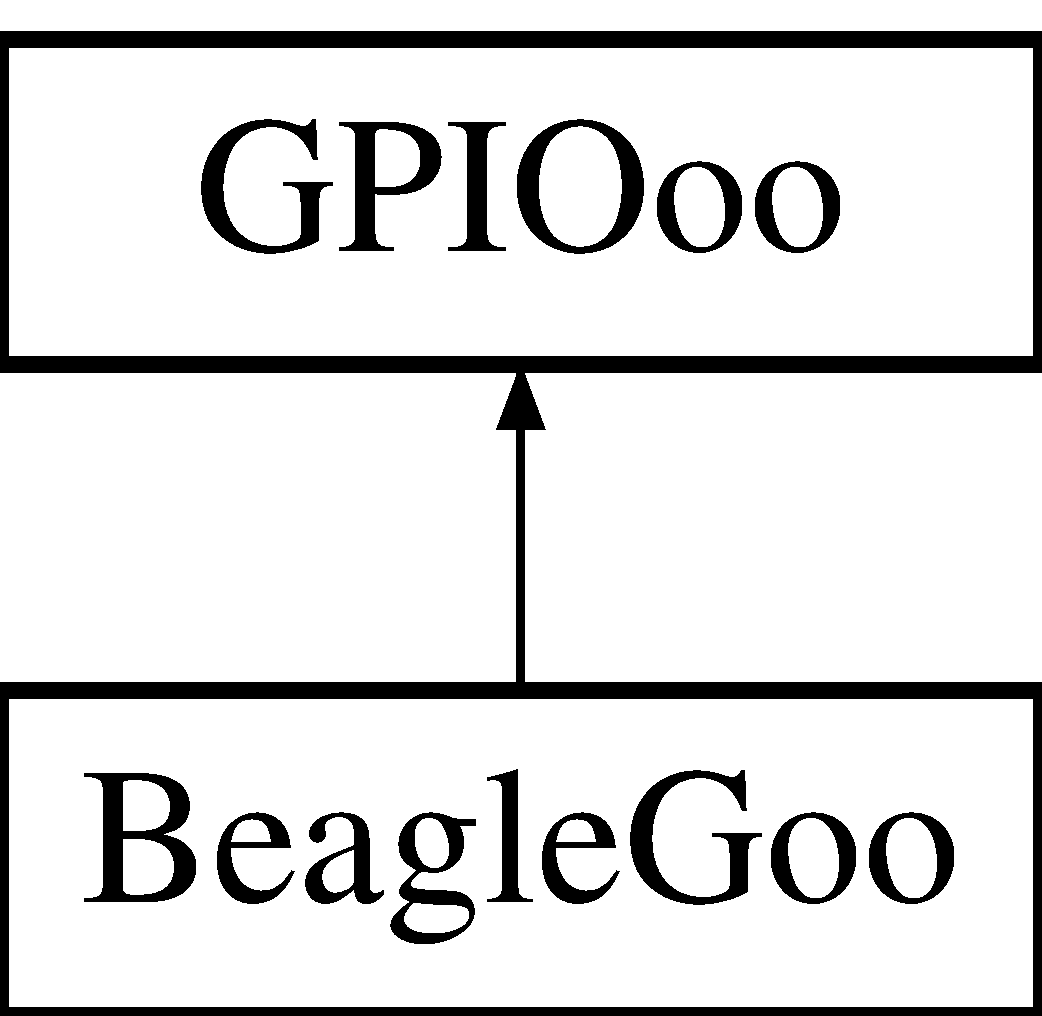
\includegraphics[height=2.000000cm]{struct_beagle_goo}
\end{center}
\end{figure}
\subsection*{Classes}
\begin{DoxyCompactItemize}
\item 
struct \hyperlink{struct_beagle_goo_1_1_g_p_i_o_info}{G\-P\-I\-O\-Info}
\end{DoxyCompactItemize}
\subsection*{Public Member Functions}
\begin{DoxyCompactItemize}
\item 
virtual \hyperlink{struct_beagle_goo_a19514c99eb2f17004ad19ffb2cd0b1d5}{$\sim$\-Beagle\-Goo} ()
\item 
virtual \hyperlink{class_g_p_i_opin}{G\-P\-I\-Opin} $\ast$ \hyperlink{struct_beagle_goo_aa5aa13bba2ba0bc364202c7856410463}{claim} (char $\ast$names\mbox{[}$\,$\mbox{]}, int num, \hyperlink{class_g_p_i_ooo_ad4b133662b68989435bcd422feb0fc03}{gpio\-Write\-Semantics} semantics, \hyperlink{class_g_p_i_ooo_a63b72558d40ed7f3ccc0c6f11d1e3b10}{gpio\-Flags} flags=\hyperlink{class_g_p_i_ooo_a63b72558d40ed7f3ccc0c6f11d1e3b10aa64ecca268265aa77389ee957e01fd63}{gpio\-Flags\-None})
\begin{DoxyCompactList}\small\item\em Method allocates G\-P\-I\-O pins and returns a G\-P\-I\-O\-Pin object. Method allocates a block of pins specified by names passed in {\itshape names} argument. Number of pins in the block is determined by {\itshape num} argument. If flag {\itshape gpio\-Exclusive} is present, only non-\/allocated pins can be allocated, the pins are marked as exclusive and can not be shared with other blocks. If the {\itshape gpio\-Exclusive} flag has not been specified, pins can be shared with other blocks. If sharing conflict has been detected, no pins must be allocated and the method must return N\-U\-L\-L. Argument {\itshape semantics} determines how write operations should be handled. If the requested write semantics is not supported by the hardware platfoom, no pins must be allocated and method must return N\-U\-L\-L. \end{DoxyCompactList}\item 
virtual void \hyperlink{struct_beagle_goo_a67436fe547740cf9ff11f5942175b2fc}{release} (\hyperlink{class_g_p_i_opin}{G\-P\-I\-Opin} $\ast$$\ast$gpio)
\begin{DoxyCompactList}\small\item\em Releases a block of G\-P\-I\-O pins. Method releases allocated block of G\-P\-I\-O pins. Methods releases memory allocated for the block, destroys the object and assigns N\-U\-L\-L to the referencing variable. \end{DoxyCompactList}\end{DoxyCompactItemize}
\subsection*{Protected Member Functions}
\begin{DoxyCompactItemize}
\item 
struct \hyperlink{struct_beagle_goo_1_1_g_p_i_o_info}{G\-P\-I\-O\-Info} $\ast$ \hyperlink{struct_beagle_goo_a2870e374462486c977ed462d169bbc07}{\-\_\-find\-Gpio} (char $\ast$name)
\item 
\hyperlink{struct_beagle_goo_a06b2b0e2d3b22016edb11b515fad8f0a}{Beagle\-Goo} ()
\end{DoxyCompactItemize}
\subsection*{Protected Attributes}
\begin{DoxyCompactItemize}
\item 
bool \hyperlink{struct_beagle_goo_a64e92bad467b29cb868bec64d1f6be6f}{active}
\item 
int \hyperlink{struct_beagle_goo_a1d4a232a0dbb10d38249e239c7e04788}{gpio\-Fd}
\item 
uint32\-\_\-t $\ast$ \hyperlink{struct_beagle_goo_aaa05aec2adfcadae3912e861ae35d50b}{gpios} \mbox{[}4\mbox{]}
\end{DoxyCompactItemize}
\subsection*{Static Protected Attributes}
\begin{DoxyCompactItemize}
\item 
static struct \hyperlink{struct_beagle_goo_1_1_g_p_i_o_info}{G\-P\-I\-O\-Info} \hyperlink{struct_beagle_goo_a2856c2fe9e24825ffd5691ab9a53d1f8}{gpio\-Infos} \mbox{[}$\,$\mbox{]}
\item 
static uint16\-\_\-t \hyperlink{struct_beagle_goo_a13b31f0a40c07bd0ca8c9d9fa51ae60a}{addrs} \mbox{[}$\,$\mbox{]}
\item 
static const uint32\-\_\-t \hyperlink{struct_beagle_goo_a709c4761b20d2db44096036573d3285f}{gpio\-Addrs} \mbox{[}$\,$\mbox{]}
\item 
static const int \hyperlink{struct_beagle_goo_ae4b9d09b2bfaf386c5d6fb9fdee0d4fa}{Max\-Gpio\-Name\-Len} = 32
\item 
static const int \hyperlink{struct_beagle_goo_a0d7150aa275f183b3c552ab89584f272}{Gpio\-Mem\-Block\-Length} = 0xfff
\end{DoxyCompactItemize}
\subsection*{Friends}
\begin{DoxyCompactItemize}
\item 
class \hyperlink{struct_beagle_goo_a3c53b8008fd7b4a4dc43d5c025cfb91f}{Beagle\-Goo\-P}
\item 
class \hyperlink{struct_beagle_goo_ad655c01bbbf0f8f066500cb0ea296455}{G\-P\-I\-Ooo}
\end{DoxyCompactItemize}
\subsection*{Additional Inherited Members}


\subsection{Detailed Description}
pin info 

\subsection{Constructor \& Destructor Documentation}
\hypertarget{struct_beagle_goo_a06b2b0e2d3b22016edb11b515fad8f0a}{\index{Beagle\-Goo@{Beagle\-Goo}!Beagle\-Goo@{Beagle\-Goo}}
\index{Beagle\-Goo@{Beagle\-Goo}!BeagleGoo@{Beagle\-Goo}}
\subsubsection[{Beagle\-Goo}]{\setlength{\rightskip}{0pt plus 5cm}Beagle\-Goo\-::\-Beagle\-Goo (
\begin{DoxyParamCaption}
{}
\end{DoxyParamCaption}
)\hspace{0.3cm}{\ttfamily [protected]}}}\label{struct_beagle_goo_a06b2b0e2d3b22016edb11b515fad8f0a}
\hypertarget{struct_beagle_goo_a19514c99eb2f17004ad19ffb2cd0b1d5}{\index{Beagle\-Goo@{Beagle\-Goo}!$\sim$\-Beagle\-Goo@{$\sim$\-Beagle\-Goo}}
\index{$\sim$\-Beagle\-Goo@{$\sim$\-Beagle\-Goo}!BeagleGoo@{Beagle\-Goo}}
\subsubsection[{$\sim$\-Beagle\-Goo}]{\setlength{\rightskip}{0pt plus 5cm}Beagle\-Goo\-::$\sim$\-Beagle\-Goo (
\begin{DoxyParamCaption}
{}
\end{DoxyParamCaption}
)\hspace{0.3cm}{\ttfamily [virtual]}}}\label{struct_beagle_goo_a19514c99eb2f17004ad19ffb2cd0b1d5}


\subsection{Member Function Documentation}
\hypertarget{struct_beagle_goo_a2870e374462486c977ed462d169bbc07}{\index{Beagle\-Goo@{Beagle\-Goo}!\-\_\-find\-Gpio@{\-\_\-find\-Gpio}}
\index{\-\_\-find\-Gpio@{\-\_\-find\-Gpio}!BeagleGoo@{Beagle\-Goo}}
\subsubsection[{\-\_\-find\-Gpio}]{\setlength{\rightskip}{0pt plus 5cm}struct {\bf Beagle\-Goo\-::\-G\-P\-I\-O\-Info} $\ast$ Beagle\-Goo\-::\-\_\-find\-Gpio (
\begin{DoxyParamCaption}
\item[{char $\ast$}]{name}
\end{DoxyParamCaption}
)\hspace{0.3cm}{\ttfamily [read]}, {\ttfamily [protected]}}}\label{struct_beagle_goo_a2870e374462486c977ed462d169bbc07}
\hypertarget{struct_beagle_goo_aa5aa13bba2ba0bc364202c7856410463}{\index{Beagle\-Goo@{Beagle\-Goo}!claim@{claim}}
\index{claim@{claim}!BeagleGoo@{Beagle\-Goo}}
\subsubsection[{claim}]{\setlength{\rightskip}{0pt plus 5cm}{\bf G\-P\-I\-Opin} $\ast$ Beagle\-Goo\-::claim (
\begin{DoxyParamCaption}
\item[{char $\ast$}]{names\mbox{[}$\,$\mbox{]}, }
\item[{int}]{num, }
\item[{{\bf gpio\-Write\-Semantics}}]{semantics, }
\item[{{\bf gpio\-Flags}}]{flags = {\ttfamily {\bf gpio\-Flags\-None}}}
\end{DoxyParamCaption}
)\hspace{0.3cm}{\ttfamily [virtual]}}}\label{struct_beagle_goo_aa5aa13bba2ba0bc364202c7856410463}


Method allocates G\-P\-I\-O pins and returns a G\-P\-I\-O\-Pin object. Method allocates a block of pins specified by names passed in {\itshape names} argument. Number of pins in the block is determined by {\itshape num} argument. If flag {\itshape gpio\-Exclusive} is present, only non-\/allocated pins can be allocated, the pins are marked as exclusive and can not be shared with other blocks. If the {\itshape gpio\-Exclusive} flag has not been specified, pins can be shared with other blocks. If sharing conflict has been detected, no pins must be allocated and the method must return N\-U\-L\-L. Argument {\itshape semantics} determines how write operations should be handled. If the requested write semantics is not supported by the hardware platfoom, no pins must be allocated and method must return N\-U\-L\-L. 


\begin{DoxyParams}{Parameters}
{\em names} & -\/ an array of system names of pins in the block. Pin names are implementation-\/dependent. The array should have {\itshape num} entries. \\
\hline
{\em num} & -\/ number of pins in the block. \\
\hline
{\em semantics} & -\/ write semantics. Uses constants defined by {\itshape gpio\-Write\-Semantics} enum. \\
\hline
{\em flags} & -\/ Flags governing pin allocation. Defined by {\itshape gpio\-Flags} enum. Optional parameter. Default value is no flags. \\
\hline
\end{DoxyParams}
\begin{DoxyReturn}{Returns}

\end{DoxyReturn}


Implements \hyperlink{class_g_p_i_ooo_a8d7ac44872a6d12ad439afe4e914f07e}{G\-P\-I\-Ooo}.

\hypertarget{struct_beagle_goo_a67436fe547740cf9ff11f5942175b2fc}{\index{Beagle\-Goo@{Beagle\-Goo}!release@{release}}
\index{release@{release}!BeagleGoo@{Beagle\-Goo}}
\subsubsection[{release}]{\setlength{\rightskip}{0pt plus 5cm}void Beagle\-Goo\-::release (
\begin{DoxyParamCaption}
\item[{{\bf G\-P\-I\-Opin} $\ast$$\ast$}]{gpio}
\end{DoxyParamCaption}
)\hspace{0.3cm}{\ttfamily [virtual]}}}\label{struct_beagle_goo_a67436fe547740cf9ff11f5942175b2fc}


Releases a block of G\-P\-I\-O pins. Method releases allocated block of G\-P\-I\-O pins. Methods releases memory allocated for the block, destroys the object and assigns N\-U\-L\-L to the referencing variable. 


\begin{DoxyParams}{Parameters}
{\em gpio} & -\/ pointer to a variable with reference to an object describing a block of G\-P\-I\-O pins. \\
\hline
\end{DoxyParams}


Implements \hyperlink{class_g_p_i_ooo_ab8a52d0d5ef2fbb9ca92baa51174e3ee}{G\-P\-I\-Ooo}.



\subsection{Friends And Related Function Documentation}
\hypertarget{struct_beagle_goo_a3c53b8008fd7b4a4dc43d5c025cfb91f}{\index{Beagle\-Goo@{Beagle\-Goo}!Beagle\-Goo\-P@{Beagle\-Goo\-P}}
\index{Beagle\-Goo\-P@{Beagle\-Goo\-P}!BeagleGoo@{Beagle\-Goo}}
\subsubsection[{Beagle\-Goo\-P}]{\setlength{\rightskip}{0pt plus 5cm}friend class {\bf Beagle\-Goo\-P}\hspace{0.3cm}{\ttfamily [friend]}}}\label{struct_beagle_goo_a3c53b8008fd7b4a4dc43d5c025cfb91f}
\hypertarget{struct_beagle_goo_ad655c01bbbf0f8f066500cb0ea296455}{\index{Beagle\-Goo@{Beagle\-Goo}!G\-P\-I\-Ooo@{G\-P\-I\-Ooo}}
\index{G\-P\-I\-Ooo@{G\-P\-I\-Ooo}!BeagleGoo@{Beagle\-Goo}}
\subsubsection[{G\-P\-I\-Ooo}]{\setlength{\rightskip}{0pt plus 5cm}friend class {\bf G\-P\-I\-Ooo}\hspace{0.3cm}{\ttfamily [friend]}}}\label{struct_beagle_goo_ad655c01bbbf0f8f066500cb0ea296455}


\subsection{Member Data Documentation}
\hypertarget{struct_beagle_goo_a64e92bad467b29cb868bec64d1f6be6f}{\index{Beagle\-Goo@{Beagle\-Goo}!active@{active}}
\index{active@{active}!BeagleGoo@{Beagle\-Goo}}
\subsubsection[{active}]{\setlength{\rightskip}{0pt plus 5cm}bool Beagle\-Goo\-::active\hspace{0.3cm}{\ttfamily [protected]}}}\label{struct_beagle_goo_a64e92bad467b29cb868bec64d1f6be6f}
\hypertarget{struct_beagle_goo_a13b31f0a40c07bd0ca8c9d9fa51ae60a}{\index{Beagle\-Goo@{Beagle\-Goo}!addrs@{addrs}}
\index{addrs@{addrs}!BeagleGoo@{Beagle\-Goo}}
\subsubsection[{addrs}]{\setlength{\rightskip}{0pt plus 5cm}uint16\-\_\-t Beagle\-Goo\-::addrs\hspace{0.3cm}{\ttfamily [static]}, {\ttfamily [protected]}}}\label{struct_beagle_goo_a13b31f0a40c07bd0ca8c9d9fa51ae60a}
{\bfseries Initial value\-:}
\begin{DoxyCode}

        \{ 0x0818, 0x081C, 0x0808,                       
                        0x080C, 0x0890, 0x0894, 0x089C, 0x0898, 
                        0x0834, 0x0830, 0x0824, 0x0828, 0x083C, 
                        0x0838, 0x082C, 0x088C, 0x0820, 0x0884, 
                        0x0880, 0x0814, 0x0810, 0x0804, 0x0800, 
                        0x087C, 0x08E0, 0x08E8, 0x08E4, 0x08EC, 
                        0x08D8, 0x08DC, 0x08D4, 0x08CC, 0x08D0, 
                        0x08C8, 0x08C0, 0x08C4, 0x08B8, 0x08BC, 
                        0x08B0, 0x08B4, 0x08A8, 0x08AC, 0x08A0, 
                        0x08A4                                  
                \}
\end{DoxyCode}
\hypertarget{struct_beagle_goo_a709c4761b20d2db44096036573d3285f}{\index{Beagle\-Goo@{Beagle\-Goo}!gpio\-Addrs@{gpio\-Addrs}}
\index{gpio\-Addrs@{gpio\-Addrs}!BeagleGoo@{Beagle\-Goo}}
\subsubsection[{gpio\-Addrs}]{\setlength{\rightskip}{0pt plus 5cm}const uint32\-\_\-t Beagle\-Goo\-::gpio\-Addrs\hspace{0.3cm}{\ttfamily [static]}, {\ttfamily [protected]}}}\label{struct_beagle_goo_a709c4761b20d2db44096036573d3285f}
{\bfseries Initial value\-:}
\begin{DoxyCode}

        \{ 0x44E07000, 0x4804C000, 0x481AC000, 0x481AE000 \}
\end{DoxyCode}
Base addresses for G\-P\-I\-O blocks in memory \hypertarget{struct_beagle_goo_a1d4a232a0dbb10d38249e239c7e04788}{\index{Beagle\-Goo@{Beagle\-Goo}!gpio\-Fd@{gpio\-Fd}}
\index{gpio\-Fd@{gpio\-Fd}!BeagleGoo@{Beagle\-Goo}}
\subsubsection[{gpio\-Fd}]{\setlength{\rightskip}{0pt plus 5cm}int Beagle\-Goo\-::gpio\-Fd\hspace{0.3cm}{\ttfamily [protected]}}}\label{struct_beagle_goo_a1d4a232a0dbb10d38249e239c7e04788}
\hypertarget{struct_beagle_goo_a2856c2fe9e24825ffd5691ab9a53d1f8}{\index{Beagle\-Goo@{Beagle\-Goo}!gpio\-Infos@{gpio\-Infos}}
\index{gpio\-Infos@{gpio\-Infos}!BeagleGoo@{Beagle\-Goo}}
\subsubsection[{gpio\-Infos}]{\setlength{\rightskip}{0pt plus 5cm}struct {\bf G\-P\-I\-O\-Info} Beagle\-Goo\-::gpio\-Infos\mbox{[}$\,$\mbox{]}\hspace{0.3cm}{\ttfamily [static]}, {\ttfamily [protected]}}}\label{struct_beagle_goo_a2856c2fe9e24825ffd5691ab9a53d1f8}
\hypertarget{struct_beagle_goo_a0d7150aa275f183b3c552ab89584f272}{\index{Beagle\-Goo@{Beagle\-Goo}!Gpio\-Mem\-Block\-Length@{Gpio\-Mem\-Block\-Length}}
\index{Gpio\-Mem\-Block\-Length@{Gpio\-Mem\-Block\-Length}!BeagleGoo@{Beagle\-Goo}}
\subsubsection[{Gpio\-Mem\-Block\-Length}]{\setlength{\rightskip}{0pt plus 5cm}const int Beagle\-Goo\-::\-Gpio\-Mem\-Block\-Length = 0xfff\hspace{0.3cm}{\ttfamily [static]}, {\ttfamily [protected]}}}\label{struct_beagle_goo_a0d7150aa275f183b3c552ab89584f272}
\hypertarget{struct_beagle_goo_aaa05aec2adfcadae3912e861ae35d50b}{\index{Beagle\-Goo@{Beagle\-Goo}!gpios@{gpios}}
\index{gpios@{gpios}!BeagleGoo@{Beagle\-Goo}}
\subsubsection[{gpios}]{\setlength{\rightskip}{0pt plus 5cm}uint32\-\_\-t$\ast$ Beagle\-Goo\-::gpios\mbox{[}4\mbox{]}\hspace{0.3cm}{\ttfamily [protected]}}}\label{struct_beagle_goo_aaa05aec2adfcadae3912e861ae35d50b}
\hypertarget{struct_beagle_goo_ae4b9d09b2bfaf386c5d6fb9fdee0d4fa}{\index{Beagle\-Goo@{Beagle\-Goo}!Max\-Gpio\-Name\-Len@{Max\-Gpio\-Name\-Len}}
\index{Max\-Gpio\-Name\-Len@{Max\-Gpio\-Name\-Len}!BeagleGoo@{Beagle\-Goo}}
\subsubsection[{Max\-Gpio\-Name\-Len}]{\setlength{\rightskip}{0pt plus 5cm}const int Beagle\-Goo\-::\-Max\-Gpio\-Name\-Len = 32\hspace{0.3cm}{\ttfamily [static]}, {\ttfamily [protected]}}}\label{struct_beagle_goo_ae4b9d09b2bfaf386c5d6fb9fdee0d4fa}


The documentation for this class was generated from the following files\-:\begin{DoxyCompactItemize}
\item 
src/\hyperlink{_beagle_goo_8cpp}{Beagle\-Goo.\-cpp}\item 
include/beaglebone/\hyperlink{_beagle_goo_8h}{Beagle\-Goo.\-h}\end{DoxyCompactItemize}

\hypertarget{class_beagle_goo_p}{\section{Beagle\-Goo\-P Class Reference}
\label{class_beagle_goo_p}\index{Beagle\-Goo\-P@{Beagle\-Goo\-P}}
}


{\ttfamily \#include $<$Beagle\-Goo\-P.\-h$>$}

Inheritance diagram for Beagle\-Goo\-P\-:\begin{figure}[H]
\begin{center}
\leavevmode
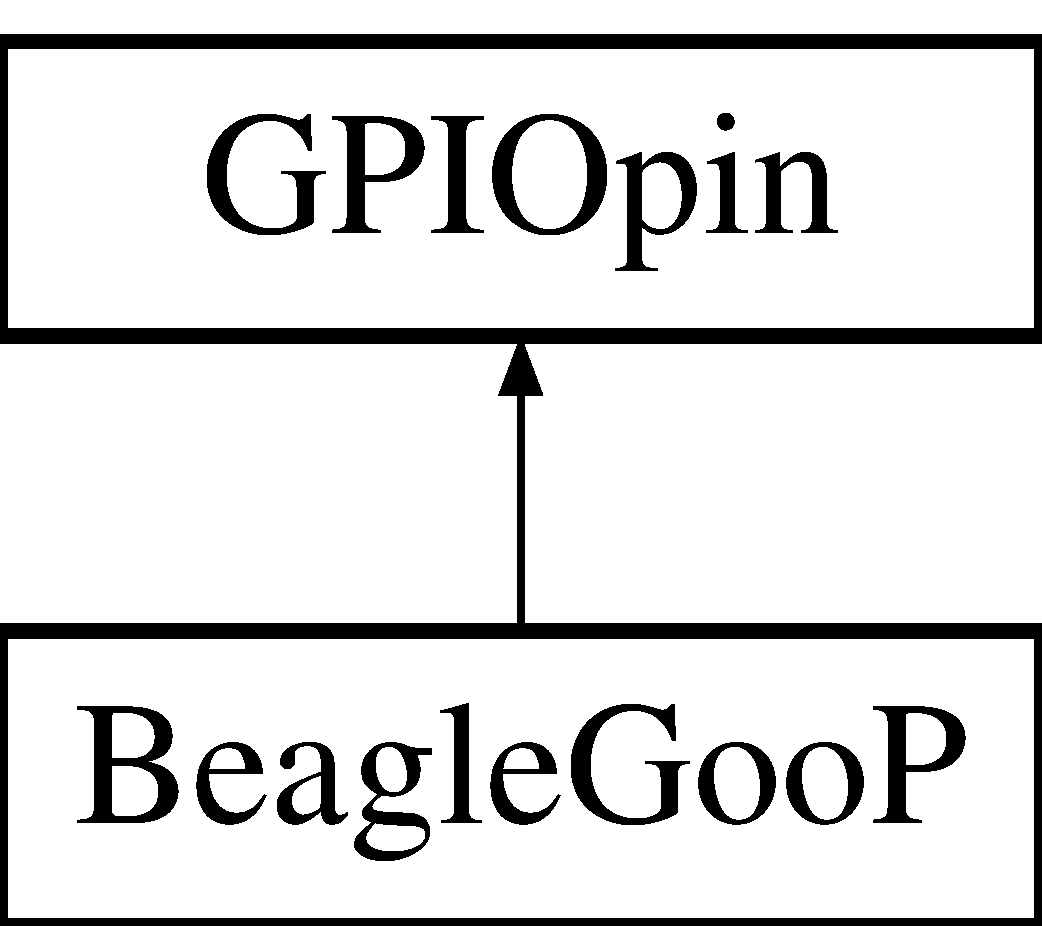
\includegraphics[height=2.000000cm]{class_beagle_goo_p}
\end{center}
\end{figure}
\subsection*{Public Member Functions}
\begin{DoxyCompactItemize}
\item 
virtual void \hyperlink{class_beagle_goo_p_a7c5b14071a87506c912b6d14f139136f}{name\-Pin} (int i, char $\ast$name)
\item 
virtual void \hyperlink{class_beagle_goo_p_a716e0b3664ed88ad427b329524311e03}{name\-Pins} (char $\ast$names\mbox{[}$\,$\mbox{]})
\item 
virtual int \hyperlink{class_beagle_goo_p_a91d2290d2c289b310d24f959371d3414}{find\-Pin\-Index} (char $\ast$name)
\item 
virtual void \hyperlink{class_beagle_goo_p_ac4d38d90c905cf318f5017b3c18203cd}{enable\-Output} (bool enable)
\item 
virtual void \hyperlink{class_beagle_goo_p_a2900cd6005cd471066d598e4866ad66f}{enable\-Output} (int i, bool enable)
\item 
virtual void \hyperlink{class_beagle_goo_p_a418b335ab7c154291a543fe18949f730}{enable\-Output} (int $\ast$outs, int num)
\item 
virtual void \hyperlink{class_beagle_goo_p_a4127207e947efe8952540fd69b949b35}{enable\-Output} (char $\ast$$\ast$out\-Names, int num)
\item 
virtual void \hyperlink{class_beagle_goo_p_a5da234ad09723ae929135e96e32cf497}{write} (uint32\-\_\-t v)
\item 
virtual void \hyperlink{class_beagle_goo_p_afa97c0b593fa9032c873654ee40140f5}{set} (uint32\-\_\-t v)
\item 
virtual void \hyperlink{class_beagle_goo_p_a8997d7bc2665b7cbd100abe613657e94}{set\-Bit} (int bit)
\item 
virtual void \hyperlink{class_beagle_goo_p_a39772670c58f71b5d7e4ca9e39eb8d86}{clear} (uint32\-\_\-t v)
\item 
virtual void \hyperlink{class_beagle_goo_p_a00a85a024ac1e9a3dbf04d4b065cc16a}{clear\-Bit} (int bit)
\item 
virtual uint32\-\_\-t \hyperlink{class_beagle_goo_p_a4a6ed00aa61f7d81de93cb880ba93d63}{read} ()
\end{DoxyCompactItemize}
\subsection*{Friends}
\begin{DoxyCompactItemize}
\item 
class \hyperlink{class_beagle_goo_p_a68d52fe38a514aef4add4867c370b174}{Beagle\-Goo}
\end{DoxyCompactItemize}
\subsection*{Additional Inherited Members}


\subsection{Member Function Documentation}
\hypertarget{class_beagle_goo_p_a39772670c58f71b5d7e4ca9e39eb8d86}{\index{Beagle\-Goo\-P@{Beagle\-Goo\-P}!clear@{clear}}
\index{clear@{clear}!BeagleGooP@{Beagle\-Goo\-P}}
\subsubsection[{clear}]{\setlength{\rightskip}{0pt plus 5cm}void Beagle\-Goo\-P\-::clear (
\begin{DoxyParamCaption}
\item[{uint32\-\_\-t}]{v}
\end{DoxyParamCaption}
)\hspace{0.3cm}{\ttfamily [virtual]}}}\label{class_beagle_goo_p_a39772670c58f71b5d7e4ca9e39eb8d86}
Method clears G\-P\-I\-O lines for which corresponding bit in the parameter {\itshape v} is set to 1. Lines whose bits are set to 0 remain unchanged. 
\begin{DoxyParams}{Parameters}
{\em v} & \\
\hline
\end{DoxyParams}


Implements \hyperlink{class_g_p_i_opin_abc101fb598fa749ae58743e8b2decbbc}{G\-P\-I\-Opin}.

\hypertarget{class_beagle_goo_p_a00a85a024ac1e9a3dbf04d4b065cc16a}{\index{Beagle\-Goo\-P@{Beagle\-Goo\-P}!clear\-Bit@{clear\-Bit}}
\index{clear\-Bit@{clear\-Bit}!BeagleGooP@{Beagle\-Goo\-P}}
\subsubsection[{clear\-Bit}]{\setlength{\rightskip}{0pt plus 5cm}void Beagle\-Goo\-P\-::clear\-Bit (
\begin{DoxyParamCaption}
\item[{int}]{bit}
\end{DoxyParamCaption}
)\hspace{0.3cm}{\ttfamily [virtual]}}}\label{class_beagle_goo_p_a00a85a024ac1e9a3dbf04d4b065cc16a}
Method clears bit-\/th bit. 
\begin{DoxyParams}{Parameters}
{\em bit} & \\
\hline
\end{DoxyParams}


Implements \hyperlink{class_g_p_i_opin_a7b79f39cb611f1b1e0a95c3a35dbc94b}{G\-P\-I\-Opin}.

\hypertarget{class_beagle_goo_p_ac4d38d90c905cf318f5017b3c18203cd}{\index{Beagle\-Goo\-P@{Beagle\-Goo\-P}!enable\-Output@{enable\-Output}}
\index{enable\-Output@{enable\-Output}!BeagleGooP@{Beagle\-Goo\-P}}
\subsubsection[{enable\-Output}]{\setlength{\rightskip}{0pt plus 5cm}void Beagle\-Goo\-P\-::enable\-Output (
\begin{DoxyParamCaption}
\item[{bool}]{enable}
\end{DoxyParamCaption}
)\hspace{0.3cm}{\ttfamily [virtual]}}}\label{class_beagle_goo_p_ac4d38d90c905cf318f5017b3c18203cd}
Method enables (if enable==true) or disables (enable==false) output buffers on all lines in the block 
\begin{DoxyParams}{Parameters}
{\em enable} & \\
\hline
\end{DoxyParams}


Implements \hyperlink{class_g_p_i_opin_a444117958e6fb28524deeefefe75c13b}{G\-P\-I\-Opin}.

\hypertarget{class_beagle_goo_p_a2900cd6005cd471066d598e4866ad66f}{\index{Beagle\-Goo\-P@{Beagle\-Goo\-P}!enable\-Output@{enable\-Output}}
\index{enable\-Output@{enable\-Output}!BeagleGooP@{Beagle\-Goo\-P}}
\subsubsection[{enable\-Output}]{\setlength{\rightskip}{0pt plus 5cm}void Beagle\-Goo\-P\-::enable\-Output (
\begin{DoxyParamCaption}
\item[{int}]{i, }
\item[{bool}]{enable}
\end{DoxyParamCaption}
)\hspace{0.3cm}{\ttfamily [virtual]}}}\label{class_beagle_goo_p_a2900cd6005cd471066d598e4866ad66f}
Method enables (if enable==true) or disables (enable==false) output buffers on i-\/th line in the block 
\begin{DoxyParams}{Parameters}
{\em i} & \\
\hline
{\em enable} & \\
\hline
\end{DoxyParams}


Implements \hyperlink{class_g_p_i_opin_a832df9e2b1d14f8434069d952d372d6d}{G\-P\-I\-Opin}.

\hypertarget{class_beagle_goo_p_a418b335ab7c154291a543fe18949f730}{\index{Beagle\-Goo\-P@{Beagle\-Goo\-P}!enable\-Output@{enable\-Output}}
\index{enable\-Output@{enable\-Output}!BeagleGooP@{Beagle\-Goo\-P}}
\subsubsection[{enable\-Output}]{\setlength{\rightskip}{0pt plus 5cm}void Beagle\-Goo\-P\-::enable\-Output (
\begin{DoxyParamCaption}
\item[{int $\ast$}]{outs, }
\item[{int}]{num}
\end{DoxyParamCaption}
)\hspace{0.3cm}{\ttfamily [virtual]}}}\label{class_beagle_goo_p_a418b335ab7c154291a543fe18949f730}
Method enables output buffers on lines listed in the {\itshape outs} array. Output buffers on all pins from the block not listed in the array will be disabled. Array contains indexes of the output lines, number of elements in the array is {\itshape num}. 
\begin{DoxyParams}{Parameters}
{\em outs} & \\
\hline
{\em num} & \\
\hline
\end{DoxyParams}


Implements \hyperlink{class_g_p_i_opin_a4e1d95ff89bb7a2b60870c318f3740a5}{G\-P\-I\-Opin}.

\hypertarget{class_beagle_goo_p_a4127207e947efe8952540fd69b949b35}{\index{Beagle\-Goo\-P@{Beagle\-Goo\-P}!enable\-Output@{enable\-Output}}
\index{enable\-Output@{enable\-Output}!BeagleGooP@{Beagle\-Goo\-P}}
\subsubsection[{enable\-Output}]{\setlength{\rightskip}{0pt plus 5cm}void Beagle\-Goo\-P\-::enable\-Output (
\begin{DoxyParamCaption}
\item[{char $\ast$$\ast$}]{out\-Names, }
\item[{int}]{num}
\end{DoxyParamCaption}
)\hspace{0.3cm}{\ttfamily [virtual]}}}\label{class_beagle_goo_p_a4127207e947efe8952540fd69b949b35}
Method enables output buffers on lines listed in the {\itshape oot\-Names} array. Output buffers on all pins from the block not listed in the array will be disabled. Array contains references to strings with names of the output lines, number of elements in the array is {\itshape num}. 
\begin{DoxyParams}{Parameters}
{\em out\-Names} & \\
\hline
{\em num} & \\
\hline
\end{DoxyParams}


Implements \hyperlink{class_g_p_i_opin_a3ce477ef4fcfced2764c489d5262ee81}{G\-P\-I\-Opin}.

\hypertarget{class_beagle_goo_p_a91d2290d2c289b310d24f959371d3414}{\index{Beagle\-Goo\-P@{Beagle\-Goo\-P}!find\-Pin\-Index@{find\-Pin\-Index}}
\index{find\-Pin\-Index@{find\-Pin\-Index}!BeagleGooP@{Beagle\-Goo\-P}}
\subsubsection[{find\-Pin\-Index}]{\setlength{\rightskip}{0pt plus 5cm}int Beagle\-Goo\-P\-::find\-Pin\-Index (
\begin{DoxyParamCaption}
\item[{char $\ast$}]{name}
\end{DoxyParamCaption}
)\hspace{0.3cm}{\ttfamily [virtual]}}}\label{class_beagle_goo_p_a91d2290d2c289b310d24f959371d3414}


Implements \hyperlink{class_g_p_i_opin_a52fd993a558bc7dacd6b5c9060dd610f}{G\-P\-I\-Opin}.

\hypertarget{class_beagle_goo_p_a7c5b14071a87506c912b6d14f139136f}{\index{Beagle\-Goo\-P@{Beagle\-Goo\-P}!name\-Pin@{name\-Pin}}
\index{name\-Pin@{name\-Pin}!BeagleGooP@{Beagle\-Goo\-P}}
\subsubsection[{name\-Pin}]{\setlength{\rightskip}{0pt plus 5cm}void Beagle\-Goo\-P\-::name\-Pin (
\begin{DoxyParamCaption}
\item[{int}]{i, }
\item[{char $\ast$}]{name}
\end{DoxyParamCaption}
)\hspace{0.3cm}{\ttfamily [virtual]}}}\label{class_beagle_goo_p_a7c5b14071a87506c912b6d14f139136f}


Implements \hyperlink{class_g_p_i_opin_a3feb6f38bd934e63d0704c9e178b443e}{G\-P\-I\-Opin}.

\hypertarget{class_beagle_goo_p_a716e0b3664ed88ad427b329524311e03}{\index{Beagle\-Goo\-P@{Beagle\-Goo\-P}!name\-Pins@{name\-Pins}}
\index{name\-Pins@{name\-Pins}!BeagleGooP@{Beagle\-Goo\-P}}
\subsubsection[{name\-Pins}]{\setlength{\rightskip}{0pt plus 5cm}void Beagle\-Goo\-P\-::name\-Pins (
\begin{DoxyParamCaption}
\item[{char $\ast$}]{names\mbox{[}$\,$\mbox{]}}
\end{DoxyParamCaption}
)\hspace{0.3cm}{\ttfamily [virtual]}}}\label{class_beagle_goo_p_a716e0b3664ed88ad427b329524311e03}


Implements \hyperlink{class_g_p_i_opin_a6d11afb8376b7ea7c5f7996fc364f64a}{G\-P\-I\-Opin}.

\hypertarget{class_beagle_goo_p_a4a6ed00aa61f7d81de93cb880ba93d63}{\index{Beagle\-Goo\-P@{Beagle\-Goo\-P}!read@{read}}
\index{read@{read}!BeagleGooP@{Beagle\-Goo\-P}}
\subsubsection[{read}]{\setlength{\rightskip}{0pt plus 5cm}uint32\-\_\-t Beagle\-Goo\-P\-::read (
\begin{DoxyParamCaption}
{}
\end{DoxyParamCaption}
)\hspace{0.3cm}{\ttfamily [virtual]}}}\label{class_beagle_goo_p_a4a6ed00aa61f7d81de93cb880ba93d63}
Function returns value read from the G\-P\-I\-O block. \begin{DoxyReturn}{Returns}

\end{DoxyReturn}


Implements \hyperlink{class_g_p_i_opin_ac1a7a08dfd7828fc6f4384f390b75c0e}{G\-P\-I\-Opin}.

\hypertarget{class_beagle_goo_p_afa97c0b593fa9032c873654ee40140f5}{\index{Beagle\-Goo\-P@{Beagle\-Goo\-P}!set@{set}}
\index{set@{set}!BeagleGooP@{Beagle\-Goo\-P}}
\subsubsection[{set}]{\setlength{\rightskip}{0pt plus 5cm}void Beagle\-Goo\-P\-::set (
\begin{DoxyParamCaption}
\item[{uint32\-\_\-t}]{v}
\end{DoxyParamCaption}
)\hspace{0.3cm}{\ttfamily [virtual]}}}\label{class_beagle_goo_p_afa97c0b593fa9032c873654ee40140f5}
Method sets G\-P\-I\-O lines for which corresponding bit in the parameter {\itshape v} is set to 1. Lines whose bits are set to 0 remain unchanged. 
\begin{DoxyParams}{Parameters}
{\em v} & \\
\hline
\end{DoxyParams}


Implements \hyperlink{class_g_p_i_opin_a75314dc1bf78be651b660a1b8df5537a}{G\-P\-I\-Opin}.

\hypertarget{class_beagle_goo_p_a8997d7bc2665b7cbd100abe613657e94}{\index{Beagle\-Goo\-P@{Beagle\-Goo\-P}!set\-Bit@{set\-Bit}}
\index{set\-Bit@{set\-Bit}!BeagleGooP@{Beagle\-Goo\-P}}
\subsubsection[{set\-Bit}]{\setlength{\rightskip}{0pt plus 5cm}void Beagle\-Goo\-P\-::set\-Bit (
\begin{DoxyParamCaption}
\item[{int}]{bit}
\end{DoxyParamCaption}
)\hspace{0.3cm}{\ttfamily [virtual]}}}\label{class_beagle_goo_p_a8997d7bc2665b7cbd100abe613657e94}
Method sets i-\/th bit. 
\begin{DoxyParams}{Parameters}
{\em bit} & \\
\hline
\end{DoxyParams}


Implements \hyperlink{class_g_p_i_opin_a7baef314398bbff5261b41e3373e68c8}{G\-P\-I\-Opin}.

\hypertarget{class_beagle_goo_p_a5da234ad09723ae929135e96e32cf497}{\index{Beagle\-Goo\-P@{Beagle\-Goo\-P}!write@{write}}
\index{write@{write}!BeagleGooP@{Beagle\-Goo\-P}}
\subsubsection[{write}]{\setlength{\rightskip}{0pt plus 5cm}void Beagle\-Goo\-P\-::write (
\begin{DoxyParamCaption}
\item[{uint32\-\_\-t}]{v}
\end{DoxyParamCaption}
)\hspace{0.3cm}{\ttfamily [virtual]}}}\label{class_beagle_goo_p_a5da234ad09723ae929135e96e32cf497}
Function writes the value to the pin. Write semantics is determined by the semantics parameter when G\-P\-I\-Os are claimed. 
\begin{DoxyParams}{Parameters}
{\em v} & \\
\hline
\end{DoxyParams}


Implements \hyperlink{class_g_p_i_opin_a5dd506e32835b1e35edf62649f3beaa6}{G\-P\-I\-Opin}.



\subsection{Friends And Related Function Documentation}
\hypertarget{class_beagle_goo_p_a68d52fe38a514aef4add4867c370b174}{\index{Beagle\-Goo\-P@{Beagle\-Goo\-P}!Beagle\-Goo@{Beagle\-Goo}}
\index{Beagle\-Goo@{Beagle\-Goo}!BeagleGooP@{Beagle\-Goo\-P}}
\subsubsection[{Beagle\-Goo}]{\setlength{\rightskip}{0pt plus 5cm}friend class {\bf Beagle\-Goo}\hspace{0.3cm}{\ttfamily [friend]}}}\label{class_beagle_goo_p_a68d52fe38a514aef4add4867c370b174}


The documentation for this class was generated from the following files\-:\begin{DoxyCompactItemize}
\item 
include/beaglebone/\hyperlink{_beagle_goo_p_8h}{Beagle\-Goo\-P.\-h}\item 
src/\hyperlink{_beagle_goo_p_8cpp}{Beagle\-Goo\-P.\-cpp}\end{DoxyCompactItemize}

\hypertarget{struct_beagle_goo_1_1_g_p_i_o_info}{\section{Beagle\-Goo\-:\-:G\-P\-I\-O\-Info Struct Reference}
\label{struct_beagle_goo_1_1_g_p_i_o_info}\index{Beagle\-Goo\-::\-G\-P\-I\-O\-Info@{Beagle\-Goo\-::\-G\-P\-I\-O\-Info}}
}


{\ttfamily \#include $<$Beagle\-Goo.\-h$>$}

\subsection*{Public Attributes}
\begin{DoxyCompactItemize}
\item 
char $\ast$ \hyperlink{struct_beagle_goo_1_1_g_p_i_o_info_aa887aa95188facb1a445920fb544134a}{name}
\item 
int \hyperlink{struct_beagle_goo_1_1_g_p_i_o_info_a870d8a3d36706dd366eea2299ccb29fd}{gpio\-Num}
\item 
int \hyperlink{struct_beagle_goo_1_1_g_p_i_o_info_a31959d0d24502777f3286e7ccb9c8e62}{bit\-Num}
\item 
int \hyperlink{struct_beagle_goo_1_1_g_p_i_o_info_af3bbf6d94585ef4a62bd579fef8564ac}{ref\-Counter}
\item 
int \hyperlink{struct_beagle_goo_1_1_g_p_i_o_info_afeb1ff6e6ad263177a9b1bb82e7a0043}{flags}
\end{DoxyCompactItemize}


\subsection{Member Data Documentation}
\hypertarget{struct_beagle_goo_1_1_g_p_i_o_info_a31959d0d24502777f3286e7ccb9c8e62}{\index{Beagle\-Goo\-::\-G\-P\-I\-O\-Info@{Beagle\-Goo\-::\-G\-P\-I\-O\-Info}!bit\-Num@{bit\-Num}}
\index{bit\-Num@{bit\-Num}!BeagleGoo::GPIOInfo@{Beagle\-Goo\-::\-G\-P\-I\-O\-Info}}
\subsubsection[{bit\-Num}]{\setlength{\rightskip}{0pt plus 5cm}int Beagle\-Goo\-::\-G\-P\-I\-O\-Info\-::bit\-Num}}\label{struct_beagle_goo_1_1_g_p_i_o_info_a31959d0d24502777f3286e7ccb9c8e62}
\hypertarget{struct_beagle_goo_1_1_g_p_i_o_info_afeb1ff6e6ad263177a9b1bb82e7a0043}{\index{Beagle\-Goo\-::\-G\-P\-I\-O\-Info@{Beagle\-Goo\-::\-G\-P\-I\-O\-Info}!flags@{flags}}
\index{flags@{flags}!BeagleGoo::GPIOInfo@{Beagle\-Goo\-::\-G\-P\-I\-O\-Info}}
\subsubsection[{flags}]{\setlength{\rightskip}{0pt plus 5cm}int Beagle\-Goo\-::\-G\-P\-I\-O\-Info\-::flags}}\label{struct_beagle_goo_1_1_g_p_i_o_info_afeb1ff6e6ad263177a9b1bb82e7a0043}
\hypertarget{struct_beagle_goo_1_1_g_p_i_o_info_a870d8a3d36706dd366eea2299ccb29fd}{\index{Beagle\-Goo\-::\-G\-P\-I\-O\-Info@{Beagle\-Goo\-::\-G\-P\-I\-O\-Info}!gpio\-Num@{gpio\-Num}}
\index{gpio\-Num@{gpio\-Num}!BeagleGoo::GPIOInfo@{Beagle\-Goo\-::\-G\-P\-I\-O\-Info}}
\subsubsection[{gpio\-Num}]{\setlength{\rightskip}{0pt plus 5cm}int Beagle\-Goo\-::\-G\-P\-I\-O\-Info\-::gpio\-Num}}\label{struct_beagle_goo_1_1_g_p_i_o_info_a870d8a3d36706dd366eea2299ccb29fd}
\hypertarget{struct_beagle_goo_1_1_g_p_i_o_info_aa887aa95188facb1a445920fb544134a}{\index{Beagle\-Goo\-::\-G\-P\-I\-O\-Info@{Beagle\-Goo\-::\-G\-P\-I\-O\-Info}!name@{name}}
\index{name@{name}!BeagleGoo::GPIOInfo@{Beagle\-Goo\-::\-G\-P\-I\-O\-Info}}
\subsubsection[{name}]{\setlength{\rightskip}{0pt plus 5cm}char$\ast$ Beagle\-Goo\-::\-G\-P\-I\-O\-Info\-::name}}\label{struct_beagle_goo_1_1_g_p_i_o_info_aa887aa95188facb1a445920fb544134a}
\hypertarget{struct_beagle_goo_1_1_g_p_i_o_info_af3bbf6d94585ef4a62bd579fef8564ac}{\index{Beagle\-Goo\-::\-G\-P\-I\-O\-Info@{Beagle\-Goo\-::\-G\-P\-I\-O\-Info}!ref\-Counter@{ref\-Counter}}
\index{ref\-Counter@{ref\-Counter}!BeagleGoo::GPIOInfo@{Beagle\-Goo\-::\-G\-P\-I\-O\-Info}}
\subsubsection[{ref\-Counter}]{\setlength{\rightskip}{0pt plus 5cm}int Beagle\-Goo\-::\-G\-P\-I\-O\-Info\-::ref\-Counter}}\label{struct_beagle_goo_1_1_g_p_i_o_info_af3bbf6d94585ef4a62bd579fef8564ac}


The documentation for this struct was generated from the following file\-:\begin{DoxyCompactItemize}
\item 
include/beaglebone/\hyperlink{_beagle_goo_8h}{Beagle\-Goo.\-h}\end{DoxyCompactItemize}

\hypertarget{class_g_p_i_ooo}{\section{G\-P\-I\-Ooo Class Reference}
\label{class_g_p_i_ooo}\index{G\-P\-I\-Ooo@{G\-P\-I\-Ooo}}
}


Object-\/oriented implementation of G\-P\-I\-O Class defines interface for object-\/oriented handling of G\-P\-I\-O operations. Should be used as parent class for platform-\/specific implementations.  




{\ttfamily \#include $<$G\-P\-I\-Ooo.\-h$>$}

Inheritance diagram for G\-P\-I\-Ooo\-:\begin{figure}[H]
\begin{center}
\leavevmode
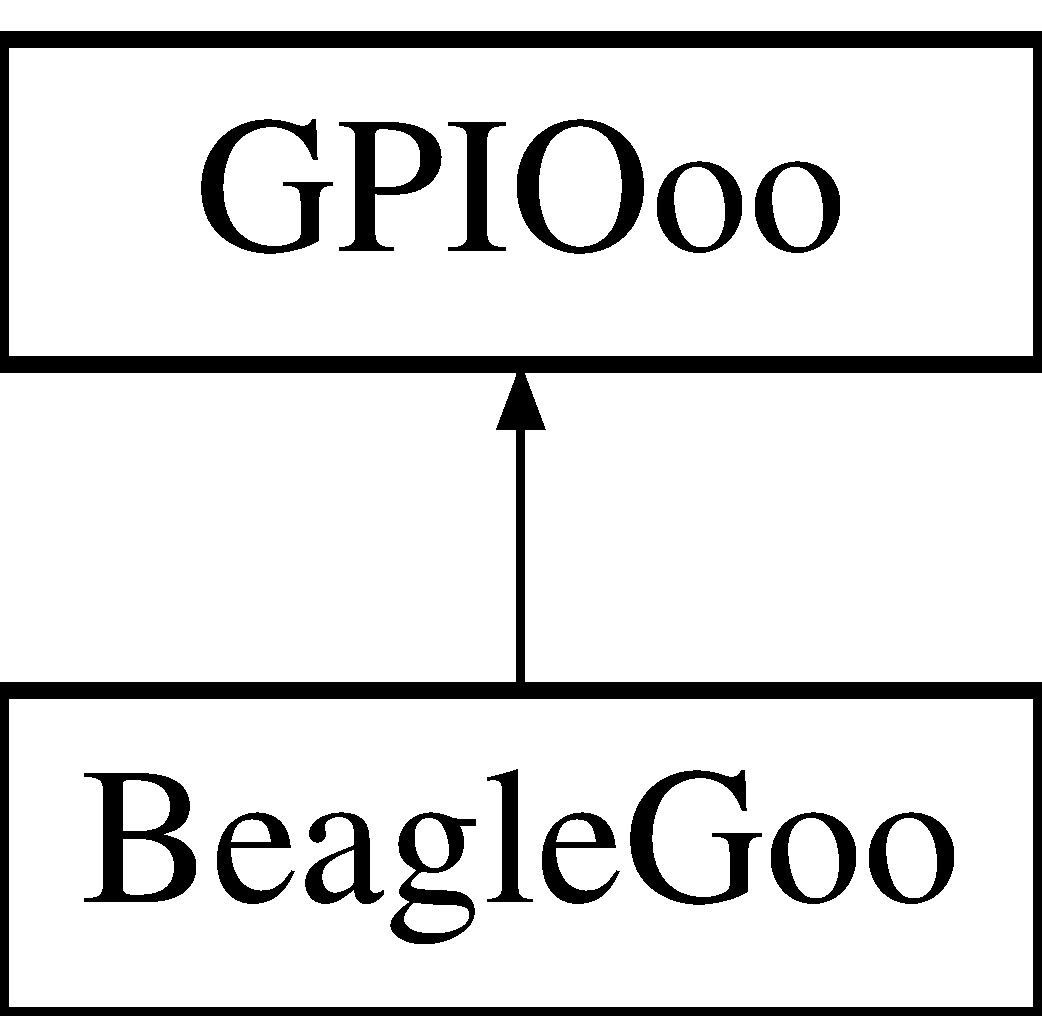
\includegraphics[height=2.000000cm]{class_g_p_i_ooo}
\end{center}
\end{figure}
\subsection*{Public Types}
\begin{DoxyCompactItemize}
\item 
enum \hyperlink{class_g_p_i_ooo_a63b72558d40ed7f3ccc0c6f11d1e3b10}{gpio\-Flags} \{ \hyperlink{class_g_p_i_ooo_a63b72558d40ed7f3ccc0c6f11d1e3b10aa64ecca268265aa77389ee957e01fd63}{gpio\-Flags\-None} = 0, 
\hyperlink{class_g_p_i_ooo_a63b72558d40ed7f3ccc0c6f11d1e3b10a42607c5a4f579963b6426f81d2266c62}{gpio\-Exclusive} = 1
 \}
\item 
enum \hyperlink{class_g_p_i_ooo_ad4b133662b68989435bcd422feb0fc03}{gpio\-Write\-Semantics} \{ \hyperlink{class_g_p_i_ooo_ad4b133662b68989435bcd422feb0fc03a21aadd48a3896150795cd7fde8c93969}{gpio\-Write} = 1, 
\hyperlink{class_g_p_i_ooo_ad4b133662b68989435bcd422feb0fc03a359f92e59dfc786c8eb730a95179fd1b}{gpio\-Write\-Atomic}, 
\hyperlink{class_g_p_i_ooo_ad4b133662b68989435bcd422feb0fc03a551b9df4fca015828bfdfbce0e4e9c31}{gpio\-Write\-Set\-Before\-Clear}, 
\hyperlink{class_g_p_i_ooo_ad4b133662b68989435bcd422feb0fc03a4b8a43356457a0d5e5994ab8f1341a7f}{gpio\-Write\-Clear\-Before\-Set}
 \}
\end{DoxyCompactItemize}
\subsection*{Public Member Functions}
\begin{DoxyCompactItemize}
\item 
virtual \hyperlink{class_g_p_i_ooo_a99319510b178ed4e1dfc448e53a6c4b3}{$\sim$\-G\-P\-I\-Ooo} ()
\item 
virtual \hyperlink{class_g_p_i_opin}{G\-P\-I\-Opin} $\ast$ \hyperlink{class_g_p_i_ooo_a07164321fda879306394d7550454dbb2}{claim} (char $\ast$names\mbox{[}$\,$\mbox{]}, int num)
\begin{DoxyCompactList}\small\item\em Simplified version of G\-P\-I\-Opin\-::claim() Simplified version of G\-P\-I\-Opin\-::claim(). Assumes {\itshape gpio\-Write} semantics and no options. \end{DoxyCompactList}\item 
virtual \hyperlink{class_g_p_i_opin}{G\-P\-I\-Opin} $\ast$ \hyperlink{class_g_p_i_ooo_a8d7ac44872a6d12ad439afe4e914f07e}{claim} (char $\ast$names\mbox{[}$\,$\mbox{]}, int num, \hyperlink{class_g_p_i_ooo_ad4b133662b68989435bcd422feb0fc03}{gpio\-Write\-Semantics} semantics, \hyperlink{class_g_p_i_ooo_a63b72558d40ed7f3ccc0c6f11d1e3b10}{gpio\-Flags} flags=\hyperlink{class_g_p_i_ooo_a63b72558d40ed7f3ccc0c6f11d1e3b10aa64ecca268265aa77389ee957e01fd63}{gpio\-Flags\-None})=0
\begin{DoxyCompactList}\small\item\em Method allocates G\-P\-I\-O pins and returns a G\-P\-I\-O\-Pin object. Method allocates a block of pins specified by names passed in {\itshape names} argument. Number of pins in the block is determined by {\itshape num} argument. If flag {\itshape gpio\-Exclusive} is present, only non-\/allocated pins can be allocated, the pins are marked as exclusive and can not be shared with other blocks. If the {\itshape gpio\-Exclusive} flag has not been specified, pins can be shared with other blocks. If sharing conflict has been detected, no pins must be allocated and the method must return N\-U\-L\-L. Argument {\itshape semantics} determines how write operations should be handled. If the requested write semantics is not supported by the hardware platfoom, no pins must be allocated and method must return N\-U\-L\-L. \end{DoxyCompactList}\item 
virtual void \hyperlink{class_g_p_i_ooo_ab8a52d0d5ef2fbb9ca92baa51174e3ee}{release} (\hyperlink{class_g_p_i_opin}{G\-P\-I\-Opin} $\ast$$\ast$gpio)=0
\begin{DoxyCompactList}\small\item\em Releases a block of G\-P\-I\-O pins. Method releases allocated block of G\-P\-I\-O pins. Methods releases memory allocated for the block, destroys the object and assigns N\-U\-L\-L to the referencing variable. \end{DoxyCompactList}\end{DoxyCompactItemize}
\subsection*{Static Public Member Functions}
\begin{DoxyCompactItemize}
\item 
static \hyperlink{class_g_p_i_ooo}{G\-P\-I\-Ooo} $\ast$ \hyperlink{class_g_p_i_ooo_a6bbf91045352182749934096c3f4c42d}{get\-Instance} ()
\end{DoxyCompactItemize}
\subsection*{Static Protected Member Functions}
\begin{DoxyCompactItemize}
\item 
static class \hyperlink{struct_beagle_goo}{Beagle\-Goo} \hyperlink{class_g_p_i_ooo_a8b49cf33628e0cb0e77c534ad971eef9}{inst} ()
\end{DoxyCompactItemize}
\subsection*{Friends}
\begin{DoxyCompactItemize}
\item 
class \hyperlink{class_g_p_i_ooo_a266ea875ace024757dd1209ea5c0a327}{G\-P\-I\-Opin}
\end{DoxyCompactItemize}


\subsection{Detailed Description}
Object-\/oriented implementation of G\-P\-I\-O Class defines interface for object-\/oriented handling of G\-P\-I\-O operations. Should be used as parent class for platform-\/specific implementations. 

\subsection{Member Enumeration Documentation}
\hypertarget{class_g_p_i_ooo_a63b72558d40ed7f3ccc0c6f11d1e3b10}{\index{G\-P\-I\-Ooo@{G\-P\-I\-Ooo}!gpio\-Flags@{gpio\-Flags}}
\index{gpio\-Flags@{gpio\-Flags}!GPIOoo@{G\-P\-I\-Ooo}}
\subsubsection[{gpio\-Flags}]{\setlength{\rightskip}{0pt plus 5cm}enum {\bf G\-P\-I\-Ooo\-::gpio\-Flags}}}\label{class_g_p_i_ooo_a63b72558d40ed7f3ccc0c6f11d1e3b10}
Options flags for G\-P\-I\-O pin allocation. \begin{Desc}
\item[Enumerator]\par
\begin{description}
\index{gpio\-Flags\-None@{gpio\-Flags\-None}!G\-P\-I\-Ooo@{G\-P\-I\-Ooo}}\index{G\-P\-I\-Ooo@{G\-P\-I\-Ooo}!gpio\-Flags\-None@{gpio\-Flags\-None}}\item[{\em 
\hypertarget{class_g_p_i_ooo_a63b72558d40ed7f3ccc0c6f11d1e3b10aa64ecca268265aa77389ee957e01fd63}{gpio\-Flags\-None}\label{class_g_p_i_ooo_a63b72558d40ed7f3ccc0c6f11d1e3b10aa64ecca268265aa77389ee957e01fd63}
}]gpio\-Flags\-None -\/ No flags \index{gpio\-Exclusive@{gpio\-Exclusive}!G\-P\-I\-Ooo@{G\-P\-I\-Ooo}}\index{G\-P\-I\-Ooo@{G\-P\-I\-Ooo}!gpio\-Exclusive@{gpio\-Exclusive}}\item[{\em 
\hypertarget{class_g_p_i_ooo_a63b72558d40ed7f3ccc0c6f11d1e3b10a42607c5a4f579963b6426f81d2266c62}{gpio\-Exclusive}\label{class_g_p_i_ooo_a63b72558d40ed7f3ccc0c6f11d1e3b10a42607c5a4f579963b6426f81d2266c62}
}]gpio\-Exclusive -\/ G\-P\-I\-Os allocated exclusively. Allocating with this flag disables sharing with other blocks. \end{description}
\end{Desc}
\hypertarget{class_g_p_i_ooo_ad4b133662b68989435bcd422feb0fc03}{\index{G\-P\-I\-Ooo@{G\-P\-I\-Ooo}!gpio\-Write\-Semantics@{gpio\-Write\-Semantics}}
\index{gpio\-Write\-Semantics@{gpio\-Write\-Semantics}!GPIOoo@{G\-P\-I\-Ooo}}
\subsubsection[{gpio\-Write\-Semantics}]{\setlength{\rightskip}{0pt plus 5cm}enum {\bf G\-P\-I\-Ooo\-::gpio\-Write\-Semantics}}}\label{class_g_p_i_ooo_ad4b133662b68989435bcd422feb0fc03}
Enum defines semantics of write operation to G\-P\-I\-Os. \begin{Desc}
\item[Enumerator]\par
\begin{description}
\index{gpio\-Write@{gpio\-Write}!G\-P\-I\-Ooo@{G\-P\-I\-Ooo}}\index{G\-P\-I\-Ooo@{G\-P\-I\-Ooo}!gpio\-Write@{gpio\-Write}}\item[{\em 
\hypertarget{class_g_p_i_ooo_ad4b133662b68989435bcd422feb0fc03a21aadd48a3896150795cd7fde8c93969}{gpio\-Write}\label{class_g_p_i_ooo_ad4b133662b68989435bcd422feb0fc03a21aadd48a3896150795cd7fde8c93969}
}]State of the port can be affected by writes to the pins on the same G\-P\-I\-O port. gpio\-Write -\/ Simple write to the port. Prone to race conditions, offers no multi-\/process safety. \index{gpio\-Write\-Atomic@{gpio\-Write\-Atomic}!G\-P\-I\-Ooo@{G\-P\-I\-Ooo}}\index{G\-P\-I\-Ooo@{G\-P\-I\-Ooo}!gpio\-Write\-Atomic@{gpio\-Write\-Atomic}}\item[{\em 
\hypertarget{class_g_p_i_ooo_ad4b133662b68989435bcd422feb0fc03a359f92e59dfc786c8eb730a95179fd1b}{gpio\-Write\-Atomic}\label{class_g_p_i_ooo_ad4b133662b68989435bcd422feb0fc03a359f92e59dfc786c8eb730a95179fd1b}
}]gpio\-Write\-Atomic -\/ Atomic write to the port. Write to the port must be guaranteed to be successful and effective. \index{gpio\-Write\-Set\-Before\-Clear@{gpio\-Write\-Set\-Before\-Clear}!G\-P\-I\-Ooo@{G\-P\-I\-Ooo}}\index{G\-P\-I\-Ooo@{G\-P\-I\-Ooo}!gpio\-Write\-Set\-Before\-Clear@{gpio\-Write\-Set\-Before\-Clear}}\item[{\em 
\hypertarget{class_g_p_i_ooo_ad4b133662b68989435bcd422feb0fc03a551b9df4fca015828bfdfbce0e4e9c31}{gpio\-Write\-Set\-Before\-Clear}\label{class_g_p_i_ooo_ad4b133662b68989435bcd422feb0fc03a551b9df4fca015828bfdfbce0e4e9c31}
}]gpio\-Write\-Set\-Before\-Clear -\/ In two-\/step implementation of writing to the pins, pins with value '1' are set before pins with value '0' are cleared. For a short period of time the state of the pins in the G\-P\-I\-O block will be equal to bitwise O\-R of the previous and next states. \index{gpio\-Write\-Clear\-Before\-Set@{gpio\-Write\-Clear\-Before\-Set}!G\-P\-I\-Ooo@{G\-P\-I\-Ooo}}\index{G\-P\-I\-Ooo@{G\-P\-I\-Ooo}!gpio\-Write\-Clear\-Before\-Set@{gpio\-Write\-Clear\-Before\-Set}}\item[{\em 
\hypertarget{class_g_p_i_ooo_ad4b133662b68989435bcd422feb0fc03a4b8a43356457a0d5e5994ab8f1341a7f}{gpio\-Write\-Clear\-Before\-Set}\label{class_g_p_i_ooo_ad4b133662b68989435bcd422feb0fc03a4b8a43356457a0d5e5994ab8f1341a7f}
}]gpio\-Write\-Clear\-Before\-Set -\/ In two-\/step implementation of writing to the pins, pins with value '0' are cleared before pins with value '1' are set. For a short period of time the state of the pins in the G\-P\-I\-O block will be equal to bitwise A\-N\-D of the previous and next states. \end{description}
\end{Desc}


\subsection{Constructor \& Destructor Documentation}
\hypertarget{class_g_p_i_ooo_a99319510b178ed4e1dfc448e53a6c4b3}{\index{G\-P\-I\-Ooo@{G\-P\-I\-Ooo}!$\sim$\-G\-P\-I\-Ooo@{$\sim$\-G\-P\-I\-Ooo}}
\index{$\sim$\-G\-P\-I\-Ooo@{$\sim$\-G\-P\-I\-Ooo}!GPIOoo@{G\-P\-I\-Ooo}}
\subsubsection[{$\sim$\-G\-P\-I\-Ooo}]{\setlength{\rightskip}{0pt plus 5cm}G\-P\-I\-Ooo\-::$\sim$\-G\-P\-I\-Ooo (
\begin{DoxyParamCaption}
{}
\end{DoxyParamCaption}
)\hspace{0.3cm}{\ttfamily [virtual]}}}\label{class_g_p_i_ooo_a99319510b178ed4e1dfc448e53a6c4b3}


\subsection{Member Function Documentation}
\hypertarget{class_g_p_i_ooo_a07164321fda879306394d7550454dbb2}{\index{G\-P\-I\-Ooo@{G\-P\-I\-Ooo}!claim@{claim}}
\index{claim@{claim}!GPIOoo@{G\-P\-I\-Ooo}}
\subsubsection[{claim}]{\setlength{\rightskip}{0pt plus 5cm}virtual {\bf G\-P\-I\-Opin}$\ast$ G\-P\-I\-Ooo\-::claim (
\begin{DoxyParamCaption}
\item[{char $\ast$}]{names\mbox{[}$\,$\mbox{]}, }
\item[{int}]{num}
\end{DoxyParamCaption}
)\hspace{0.3cm}{\ttfamily [inline]}, {\ttfamily [virtual]}}}\label{class_g_p_i_ooo_a07164321fda879306394d7550454dbb2}


Simplified version of G\-P\-I\-Opin\-::claim() Simplified version of G\-P\-I\-Opin\-::claim(). Assumes {\itshape gpio\-Write} semantics and no options. 


\begin{DoxyParams}{Parameters}
{\em names} & -\/ an array of system names of pins in the block. Pin names are implementation-\/dependent. The array should have {\itshape num} entries. \\
\hline
{\em num} & -\/ number of pins in the block. \\
\hline
\end{DoxyParams}
\begin{DoxyReturn}{Returns}

\end{DoxyReturn}
\hypertarget{class_g_p_i_ooo_a8d7ac44872a6d12ad439afe4e914f07e}{\index{G\-P\-I\-Ooo@{G\-P\-I\-Ooo}!claim@{claim}}
\index{claim@{claim}!GPIOoo@{G\-P\-I\-Ooo}}
\subsubsection[{claim}]{\setlength{\rightskip}{0pt plus 5cm}virtual {\bf G\-P\-I\-Opin}$\ast$ G\-P\-I\-Ooo\-::claim (
\begin{DoxyParamCaption}
\item[{char $\ast$}]{names\mbox{[}$\,$\mbox{]}, }
\item[{int}]{num, }
\item[{{\bf gpio\-Write\-Semantics}}]{semantics, }
\item[{{\bf gpio\-Flags}}]{flags = {\ttfamily {\bf gpio\-Flags\-None}}}
\end{DoxyParamCaption}
)\hspace{0.3cm}{\ttfamily [pure virtual]}}}\label{class_g_p_i_ooo_a8d7ac44872a6d12ad439afe4e914f07e}


Method allocates G\-P\-I\-O pins and returns a G\-P\-I\-O\-Pin object. Method allocates a block of pins specified by names passed in {\itshape names} argument. Number of pins in the block is determined by {\itshape num} argument. If flag {\itshape gpio\-Exclusive} is present, only non-\/allocated pins can be allocated, the pins are marked as exclusive and can not be shared with other blocks. If the {\itshape gpio\-Exclusive} flag has not been specified, pins can be shared with other blocks. If sharing conflict has been detected, no pins must be allocated and the method must return N\-U\-L\-L. Argument {\itshape semantics} determines how write operations should be handled. If the requested write semantics is not supported by the hardware platfoom, no pins must be allocated and method must return N\-U\-L\-L. 


\begin{DoxyParams}{Parameters}
{\em names} & -\/ an array of system names of pins in the block. Pin names are implementation-\/dependent. The array should have {\itshape num} entries. \\
\hline
{\em num} & -\/ number of pins in the block. \\
\hline
{\em semantics} & -\/ write semantics. Uses constants defined by {\itshape gpio\-Write\-Semantics} enum. \\
\hline
{\em flags} & -\/ Flags governing pin allocation. Defined by {\itshape gpio\-Flags} enum. Optional parameter. Default value is no flags. \\
\hline
\end{DoxyParams}
\begin{DoxyReturn}{Returns}

\end{DoxyReturn}


Implemented in \hyperlink{struct_beagle_goo_aa5aa13bba2ba0bc364202c7856410463}{Beagle\-Goo}.

\hypertarget{class_g_p_i_ooo_a6bbf91045352182749934096c3f4c42d}{\index{G\-P\-I\-Ooo@{G\-P\-I\-Ooo}!get\-Instance@{get\-Instance}}
\index{get\-Instance@{get\-Instance}!GPIOoo@{G\-P\-I\-Ooo}}
\subsubsection[{get\-Instance}]{\setlength{\rightskip}{0pt plus 5cm}class {\bf G\-P\-I\-Ooo} $\ast$ G\-P\-I\-Ooo\-::get\-Instance (
\begin{DoxyParamCaption}
{}
\end{DoxyParamCaption}
)\hspace{0.3cm}{\ttfamily [static]}}}\label{class_g_p_i_ooo_a6bbf91045352182749934096c3f4c42d}
\hypertarget{class_g_p_i_ooo_a8b49cf33628e0cb0e77c534ad971eef9}{\index{G\-P\-I\-Ooo@{G\-P\-I\-Ooo}!inst@{inst}}
\index{inst@{inst}!GPIOoo@{G\-P\-I\-Ooo}}
\subsubsection[{inst}]{\setlength{\rightskip}{0pt plus 5cm}static class {\bf Beagle\-Goo} G\-P\-I\-Ooo\-::inst (
\begin{DoxyParamCaption}
{}
\end{DoxyParamCaption}
)\hspace{0.3cm}{\ttfamily [static]}, {\ttfamily [protected]}}}\label{class_g_p_i_ooo_a8b49cf33628e0cb0e77c534ad971eef9}
\hypertarget{class_g_p_i_ooo_ab8a52d0d5ef2fbb9ca92baa51174e3ee}{\index{G\-P\-I\-Ooo@{G\-P\-I\-Ooo}!release@{release}}
\index{release@{release}!GPIOoo@{G\-P\-I\-Ooo}}
\subsubsection[{release}]{\setlength{\rightskip}{0pt plus 5cm}virtual void G\-P\-I\-Ooo\-::release (
\begin{DoxyParamCaption}
\item[{{\bf G\-P\-I\-Opin} $\ast$$\ast$}]{gpio}
\end{DoxyParamCaption}
)\hspace{0.3cm}{\ttfamily [pure virtual]}}}\label{class_g_p_i_ooo_ab8a52d0d5ef2fbb9ca92baa51174e3ee}


Releases a block of G\-P\-I\-O pins. Method releases allocated block of G\-P\-I\-O pins. Methods releases memory allocated for the block, destroys the object and assigns N\-U\-L\-L to the referencing variable. 


\begin{DoxyParams}{Parameters}
{\em gpio} & -\/ pointer to a variable with reference to an object describing a block of G\-P\-I\-O pins. \\
\hline
\end{DoxyParams}


Implemented in \hyperlink{struct_beagle_goo_a67436fe547740cf9ff11f5942175b2fc}{Beagle\-Goo}.



\subsection{Friends And Related Function Documentation}
\hypertarget{class_g_p_i_ooo_a266ea875ace024757dd1209ea5c0a327}{\index{G\-P\-I\-Ooo@{G\-P\-I\-Ooo}!G\-P\-I\-Opin@{G\-P\-I\-Opin}}
\index{G\-P\-I\-Opin@{G\-P\-I\-Opin}!GPIOoo@{G\-P\-I\-Ooo}}
\subsubsection[{G\-P\-I\-Opin}]{\setlength{\rightskip}{0pt plus 5cm}friend class {\bf G\-P\-I\-Opin}\hspace{0.3cm}{\ttfamily [friend]}}}\label{class_g_p_i_ooo_a266ea875ace024757dd1209ea5c0a327}


The documentation for this class was generated from the following files\-:\begin{DoxyCompactItemize}
\item 
include/\hyperlink{_g_p_i_ooo_8h}{G\-P\-I\-Ooo.\-h}\item 
src/\hyperlink{_g_p_i_ooo_8cpp}{G\-P\-I\-Ooo.\-cpp}\end{DoxyCompactItemize}

\hypertarget{class_g_p_i_opin}{\section{G\-P\-I\-Opin Class Reference}
\label{class_g_p_i_opin}\index{G\-P\-I\-Opin@{G\-P\-I\-Opin}}
}


{\ttfamily \#include $<$G\-P\-I\-Opin.\-h$>$}

Inheritance diagram for G\-P\-I\-Opin\-:\begin{figure}[H]
\begin{center}
\leavevmode
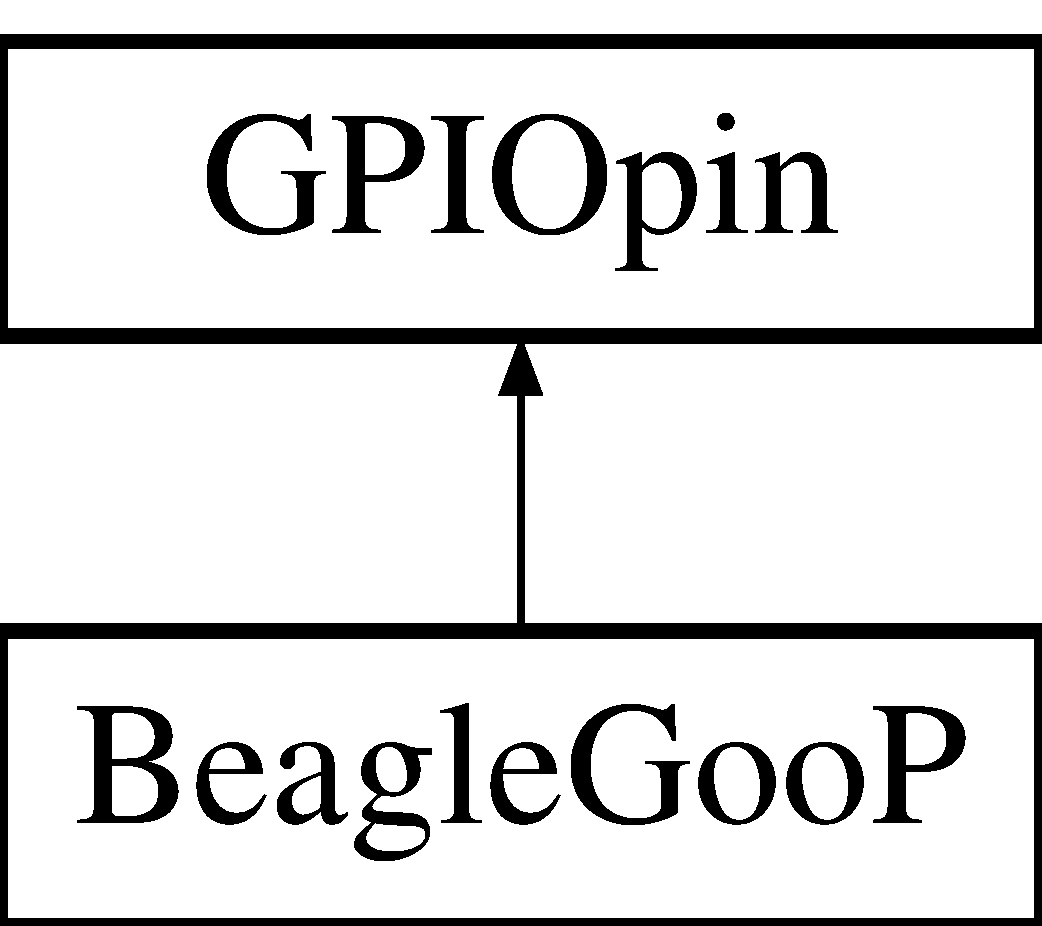
\includegraphics[height=2.000000cm]{class_g_p_i_opin}
\end{center}
\end{figure}
\subsection*{Public Member Functions}
\begin{DoxyCompactItemize}
\item 
virtual \hyperlink{class_g_p_i_opin_a28e3ff135999c7bfe6f9ebb6b2c8512e}{$\sim$\-G\-P\-I\-Opin} ()
\item 
virtual void \hyperlink{class_g_p_i_opin_a3feb6f38bd934e63d0704c9e178b443e}{name\-Pin} (int i, char $\ast$name)=0
\item 
virtual void \hyperlink{class_g_p_i_opin_a6d11afb8376b7ea7c5f7996fc364f64a}{name\-Pins} (char $\ast$names\mbox{[}$\,$\mbox{]})=0
\item 
virtual int \hyperlink{class_g_p_i_opin_a52fd993a558bc7dacd6b5c9060dd610f}{find\-Pin\-Index} (char $\ast$name)=0
\item 
virtual void \hyperlink{class_g_p_i_opin_a444117958e6fb28524deeefefe75c13b}{enable\-Output} (bool enable)=0
\item 
virtual void \hyperlink{class_g_p_i_opin_a832df9e2b1d14f8434069d952d372d6d}{enable\-Output} (int i, bool enable)=0
\item 
virtual void \hyperlink{class_g_p_i_opin_a4e1d95ff89bb7a2b60870c318f3740a5}{enable\-Output} (int $\ast$outs, int num)=0
\item 
virtual void \hyperlink{class_g_p_i_opin_a3ce477ef4fcfced2764c489d5262ee81}{enable\-Output} (char $\ast$$\ast$out\-Names, int num)=0
\item 
virtual void \hyperlink{class_g_p_i_opin_a5dd506e32835b1e35edf62649f3beaa6}{write} (uint32\-\_\-t v)=0
\item 
virtual void \hyperlink{class_g_p_i_opin_a75314dc1bf78be651b660a1b8df5537a}{set} (uint32\-\_\-t v)=0
\item 
virtual void \hyperlink{class_g_p_i_opin_a7baef314398bbff5261b41e3373e68c8}{set\-Bit} (int bit)=0
\item 
virtual void \hyperlink{class_g_p_i_opin_abc101fb598fa749ae58743e8b2decbbc}{clear} (uint32\-\_\-t v)=0
\item 
virtual void \hyperlink{class_g_p_i_opin_a7b79f39cb611f1b1e0a95c3a35dbc94b}{clear\-Bit} (int bit)=0
\item 
virtual uint32\-\_\-t \hyperlink{class_g_p_i_opin_ac1a7a08dfd7828fc6f4384f390b75c0e}{read} ()=0
\item 
bool \hyperlink{class_g_p_i_opin_aa6bfbc72b6c3d58b0e01f3fec428b1b1}{is\-Valid} ()
\end{DoxyCompactItemize}
\subsection*{Protected Member Functions}
\begin{DoxyCompactItemize}
\item 
\hyperlink{class_g_p_i_opin_ae83b7a3f257d0a621b3cf41da8e79e23}{G\-P\-I\-Opin} ()
\end{DoxyCompactItemize}
\subsection*{Protected Attributes}
\begin{DoxyCompactItemize}
\item 
bool \hyperlink{class_g_p_i_opin_ab51fd28869cad5b9fdb38a983cb2d1c5}{active}
\end{DoxyCompactItemize}
\subsection*{Friends}
\begin{DoxyCompactItemize}
\item 
class \hyperlink{class_g_p_i_opin_a44d5d3921b935cbde07cb645da31fdae}{G\-P\-I\-O}
\end{DoxyCompactItemize}


\subsection{Constructor \& Destructor Documentation}
\hypertarget{class_g_p_i_opin_ae83b7a3f257d0a621b3cf41da8e79e23}{\index{G\-P\-I\-Opin@{G\-P\-I\-Opin}!G\-P\-I\-Opin@{G\-P\-I\-Opin}}
\index{G\-P\-I\-Opin@{G\-P\-I\-Opin}!GPIOpin@{G\-P\-I\-Opin}}
\subsubsection[{G\-P\-I\-Opin}]{\setlength{\rightskip}{0pt plus 5cm}G\-P\-I\-Opin\-::\-G\-P\-I\-Opin (
\begin{DoxyParamCaption}
{}
\end{DoxyParamCaption}
)\hspace{0.3cm}{\ttfamily [inline]}, {\ttfamily [protected]}}}\label{class_g_p_i_opin_ae83b7a3f257d0a621b3cf41da8e79e23}
\hypertarget{class_g_p_i_opin_a28e3ff135999c7bfe6f9ebb6b2c8512e}{\index{G\-P\-I\-Opin@{G\-P\-I\-Opin}!$\sim$\-G\-P\-I\-Opin@{$\sim$\-G\-P\-I\-Opin}}
\index{$\sim$\-G\-P\-I\-Opin@{$\sim$\-G\-P\-I\-Opin}!GPIOpin@{G\-P\-I\-Opin}}
\subsubsection[{$\sim$\-G\-P\-I\-Opin}]{\setlength{\rightskip}{0pt plus 5cm}virtual G\-P\-I\-Opin\-::$\sim$\-G\-P\-I\-Opin (
\begin{DoxyParamCaption}
{}
\end{DoxyParamCaption}
)\hspace{0.3cm}{\ttfamily [inline]}, {\ttfamily [virtual]}}}\label{class_g_p_i_opin_a28e3ff135999c7bfe6f9ebb6b2c8512e}


\subsection{Member Function Documentation}
\hypertarget{class_g_p_i_opin_abc101fb598fa749ae58743e8b2decbbc}{\index{G\-P\-I\-Opin@{G\-P\-I\-Opin}!clear@{clear}}
\index{clear@{clear}!GPIOpin@{G\-P\-I\-Opin}}
\subsubsection[{clear}]{\setlength{\rightskip}{0pt plus 5cm}virtual void G\-P\-I\-Opin\-::clear (
\begin{DoxyParamCaption}
\item[{uint32\-\_\-t}]{v}
\end{DoxyParamCaption}
)\hspace{0.3cm}{\ttfamily [pure virtual]}}}\label{class_g_p_i_opin_abc101fb598fa749ae58743e8b2decbbc}
Method clears G\-P\-I\-O lines for which corresponding bit in the parameter {\itshape v} is set to 1. Lines whose bits are set to 0 remain unchanged. 
\begin{DoxyParams}{Parameters}
{\em v} & \\
\hline
\end{DoxyParams}


Implemented in \hyperlink{class_beagle_goo_p_a39772670c58f71b5d7e4ca9e39eb8d86}{Beagle\-Goo\-P}.

\hypertarget{class_g_p_i_opin_a7b79f39cb611f1b1e0a95c3a35dbc94b}{\index{G\-P\-I\-Opin@{G\-P\-I\-Opin}!clear\-Bit@{clear\-Bit}}
\index{clear\-Bit@{clear\-Bit}!GPIOpin@{G\-P\-I\-Opin}}
\subsubsection[{clear\-Bit}]{\setlength{\rightskip}{0pt plus 5cm}virtual void G\-P\-I\-Opin\-::clear\-Bit (
\begin{DoxyParamCaption}
\item[{int}]{bit}
\end{DoxyParamCaption}
)\hspace{0.3cm}{\ttfamily [pure virtual]}}}\label{class_g_p_i_opin_a7b79f39cb611f1b1e0a95c3a35dbc94b}
Method clears bit-\/th bit. 
\begin{DoxyParams}{Parameters}
{\em bit} & \\
\hline
\end{DoxyParams}


Implemented in \hyperlink{class_beagle_goo_p_a00a85a024ac1e9a3dbf04d4b065cc16a}{Beagle\-Goo\-P}.

\hypertarget{class_g_p_i_opin_a444117958e6fb28524deeefefe75c13b}{\index{G\-P\-I\-Opin@{G\-P\-I\-Opin}!enable\-Output@{enable\-Output}}
\index{enable\-Output@{enable\-Output}!GPIOpin@{G\-P\-I\-Opin}}
\subsubsection[{enable\-Output}]{\setlength{\rightskip}{0pt plus 5cm}virtual void G\-P\-I\-Opin\-::enable\-Output (
\begin{DoxyParamCaption}
\item[{bool}]{enable}
\end{DoxyParamCaption}
)\hspace{0.3cm}{\ttfamily [pure virtual]}}}\label{class_g_p_i_opin_a444117958e6fb28524deeefefe75c13b}
Method enables (if enable==true) or disables (enable==false) output buffers on all lines in the block 
\begin{DoxyParams}{Parameters}
{\em enable} & \\
\hline
\end{DoxyParams}


Implemented in \hyperlink{class_beagle_goo_p_ac4d38d90c905cf318f5017b3c18203cd}{Beagle\-Goo\-P}.

\hypertarget{class_g_p_i_opin_a832df9e2b1d14f8434069d952d372d6d}{\index{G\-P\-I\-Opin@{G\-P\-I\-Opin}!enable\-Output@{enable\-Output}}
\index{enable\-Output@{enable\-Output}!GPIOpin@{G\-P\-I\-Opin}}
\subsubsection[{enable\-Output}]{\setlength{\rightskip}{0pt plus 5cm}virtual void G\-P\-I\-Opin\-::enable\-Output (
\begin{DoxyParamCaption}
\item[{int}]{i, }
\item[{bool}]{enable}
\end{DoxyParamCaption}
)\hspace{0.3cm}{\ttfamily [pure virtual]}}}\label{class_g_p_i_opin_a832df9e2b1d14f8434069d952d372d6d}
Method enables (if enable==true) or disables (enable==false) output buffers on i-\/th line in the block 
\begin{DoxyParams}{Parameters}
{\em i} & \\
\hline
{\em enable} & \\
\hline
\end{DoxyParams}


Implemented in \hyperlink{class_beagle_goo_p_a2900cd6005cd471066d598e4866ad66f}{Beagle\-Goo\-P}.

\hypertarget{class_g_p_i_opin_a4e1d95ff89bb7a2b60870c318f3740a5}{\index{G\-P\-I\-Opin@{G\-P\-I\-Opin}!enable\-Output@{enable\-Output}}
\index{enable\-Output@{enable\-Output}!GPIOpin@{G\-P\-I\-Opin}}
\subsubsection[{enable\-Output}]{\setlength{\rightskip}{0pt plus 5cm}virtual void G\-P\-I\-Opin\-::enable\-Output (
\begin{DoxyParamCaption}
\item[{int $\ast$}]{outs, }
\item[{int}]{num}
\end{DoxyParamCaption}
)\hspace{0.3cm}{\ttfamily [pure virtual]}}}\label{class_g_p_i_opin_a4e1d95ff89bb7a2b60870c318f3740a5}
Method enables output buffers on lines listed in the {\itshape outs} array. Output buffers on all pins from the block not listed in the array will be disabled. Array contains indexes of the output lines, number of elements in the array is {\itshape num}. 
\begin{DoxyParams}{Parameters}
{\em outs} & \\
\hline
{\em num} & \\
\hline
\end{DoxyParams}


Implemented in \hyperlink{class_beagle_goo_p_a418b335ab7c154291a543fe18949f730}{Beagle\-Goo\-P}.

\hypertarget{class_g_p_i_opin_a3ce477ef4fcfced2764c489d5262ee81}{\index{G\-P\-I\-Opin@{G\-P\-I\-Opin}!enable\-Output@{enable\-Output}}
\index{enable\-Output@{enable\-Output}!GPIOpin@{G\-P\-I\-Opin}}
\subsubsection[{enable\-Output}]{\setlength{\rightskip}{0pt plus 5cm}virtual void G\-P\-I\-Opin\-::enable\-Output (
\begin{DoxyParamCaption}
\item[{char $\ast$$\ast$}]{out\-Names, }
\item[{int}]{num}
\end{DoxyParamCaption}
)\hspace{0.3cm}{\ttfamily [pure virtual]}}}\label{class_g_p_i_opin_a3ce477ef4fcfced2764c489d5262ee81}
Method enables output buffers on lines listed in the {\itshape oot\-Names} array. Output buffers on all pins from the block not listed in the array will be disabled. Array contains references to strings with names of the output lines, number of elements in the array is {\itshape num}. 
\begin{DoxyParams}{Parameters}
{\em out\-Names} & \\
\hline
{\em num} & \\
\hline
\end{DoxyParams}


Implemented in \hyperlink{class_beagle_goo_p_a4127207e947efe8952540fd69b949b35}{Beagle\-Goo\-P}.

\hypertarget{class_g_p_i_opin_a52fd993a558bc7dacd6b5c9060dd610f}{\index{G\-P\-I\-Opin@{G\-P\-I\-Opin}!find\-Pin\-Index@{find\-Pin\-Index}}
\index{find\-Pin\-Index@{find\-Pin\-Index}!GPIOpin@{G\-P\-I\-Opin}}
\subsubsection[{find\-Pin\-Index}]{\setlength{\rightskip}{0pt plus 5cm}virtual int G\-P\-I\-Opin\-::find\-Pin\-Index (
\begin{DoxyParamCaption}
\item[{char $\ast$}]{name}
\end{DoxyParamCaption}
)\hspace{0.3cm}{\ttfamily [pure virtual]}}}\label{class_g_p_i_opin_a52fd993a558bc7dacd6b5c9060dd610f}


Implemented in \hyperlink{class_beagle_goo_p_a91d2290d2c289b310d24f959371d3414}{Beagle\-Goo\-P}.

\hypertarget{class_g_p_i_opin_aa6bfbc72b6c3d58b0e01f3fec428b1b1}{\index{G\-P\-I\-Opin@{G\-P\-I\-Opin}!is\-Valid@{is\-Valid}}
\index{is\-Valid@{is\-Valid}!GPIOpin@{G\-P\-I\-Opin}}
\subsubsection[{is\-Valid}]{\setlength{\rightskip}{0pt plus 5cm}bool G\-P\-I\-Opin\-::is\-Valid (
\begin{DoxyParamCaption}
{}
\end{DoxyParamCaption}
)\hspace{0.3cm}{\ttfamily [inline]}}}\label{class_g_p_i_opin_aa6bfbc72b6c3d58b0e01f3fec428b1b1}
Method returns true of the block describes a valid set of G\-P\-I\-O lines. If method returns false, the block is useless and should not be expected to perform any operations. \begin{DoxyReturn}{Returns}

\end{DoxyReturn}
\hypertarget{class_g_p_i_opin_a3feb6f38bd934e63d0704c9e178b443e}{\index{G\-P\-I\-Opin@{G\-P\-I\-Opin}!name\-Pin@{name\-Pin}}
\index{name\-Pin@{name\-Pin}!GPIOpin@{G\-P\-I\-Opin}}
\subsubsection[{name\-Pin}]{\setlength{\rightskip}{0pt plus 5cm}virtual void G\-P\-I\-Opin\-::name\-Pin (
\begin{DoxyParamCaption}
\item[{int}]{i, }
\item[{char $\ast$}]{name}
\end{DoxyParamCaption}
)\hspace{0.3cm}{\ttfamily [pure virtual]}}}\label{class_g_p_i_opin_a3feb6f38bd934e63d0704c9e178b443e}


Implemented in \hyperlink{class_beagle_goo_p_a7c5b14071a87506c912b6d14f139136f}{Beagle\-Goo\-P}.

\hypertarget{class_g_p_i_opin_a6d11afb8376b7ea7c5f7996fc364f64a}{\index{G\-P\-I\-Opin@{G\-P\-I\-Opin}!name\-Pins@{name\-Pins}}
\index{name\-Pins@{name\-Pins}!GPIOpin@{G\-P\-I\-Opin}}
\subsubsection[{name\-Pins}]{\setlength{\rightskip}{0pt plus 5cm}virtual void G\-P\-I\-Opin\-::name\-Pins (
\begin{DoxyParamCaption}
\item[{char $\ast$}]{names\mbox{[}$\,$\mbox{]}}
\end{DoxyParamCaption}
)\hspace{0.3cm}{\ttfamily [pure virtual]}}}\label{class_g_p_i_opin_a6d11afb8376b7ea7c5f7996fc364f64a}


Implemented in \hyperlink{class_beagle_goo_p_a716e0b3664ed88ad427b329524311e03}{Beagle\-Goo\-P}.

\hypertarget{class_g_p_i_opin_ac1a7a08dfd7828fc6f4384f390b75c0e}{\index{G\-P\-I\-Opin@{G\-P\-I\-Opin}!read@{read}}
\index{read@{read}!GPIOpin@{G\-P\-I\-Opin}}
\subsubsection[{read}]{\setlength{\rightskip}{0pt plus 5cm}virtual uint32\-\_\-t G\-P\-I\-Opin\-::read (
\begin{DoxyParamCaption}
{}
\end{DoxyParamCaption}
)\hspace{0.3cm}{\ttfamily [pure virtual]}}}\label{class_g_p_i_opin_ac1a7a08dfd7828fc6f4384f390b75c0e}
Function returns value read from the G\-P\-I\-O block. \begin{DoxyReturn}{Returns}

\end{DoxyReturn}


Implemented in \hyperlink{class_beagle_goo_p_a4a6ed00aa61f7d81de93cb880ba93d63}{Beagle\-Goo\-P}.

\hypertarget{class_g_p_i_opin_a75314dc1bf78be651b660a1b8df5537a}{\index{G\-P\-I\-Opin@{G\-P\-I\-Opin}!set@{set}}
\index{set@{set}!GPIOpin@{G\-P\-I\-Opin}}
\subsubsection[{set}]{\setlength{\rightskip}{0pt plus 5cm}virtual void G\-P\-I\-Opin\-::set (
\begin{DoxyParamCaption}
\item[{uint32\-\_\-t}]{v}
\end{DoxyParamCaption}
)\hspace{0.3cm}{\ttfamily [pure virtual]}}}\label{class_g_p_i_opin_a75314dc1bf78be651b660a1b8df5537a}
Method sets G\-P\-I\-O lines for which corresponding bit in the parameter {\itshape v} is set to 1. Lines whose bits are set to 0 remain unchanged. 
\begin{DoxyParams}{Parameters}
{\em v} & \\
\hline
\end{DoxyParams}


Implemented in \hyperlink{class_beagle_goo_p_afa97c0b593fa9032c873654ee40140f5}{Beagle\-Goo\-P}.

\hypertarget{class_g_p_i_opin_a7baef314398bbff5261b41e3373e68c8}{\index{G\-P\-I\-Opin@{G\-P\-I\-Opin}!set\-Bit@{set\-Bit}}
\index{set\-Bit@{set\-Bit}!GPIOpin@{G\-P\-I\-Opin}}
\subsubsection[{set\-Bit}]{\setlength{\rightskip}{0pt plus 5cm}virtual void G\-P\-I\-Opin\-::set\-Bit (
\begin{DoxyParamCaption}
\item[{int}]{bit}
\end{DoxyParamCaption}
)\hspace{0.3cm}{\ttfamily [pure virtual]}}}\label{class_g_p_i_opin_a7baef314398bbff5261b41e3373e68c8}
Method sets i-\/th bit. 
\begin{DoxyParams}{Parameters}
{\em bit} & \\
\hline
\end{DoxyParams}


Implemented in \hyperlink{class_beagle_goo_p_a8997d7bc2665b7cbd100abe613657e94}{Beagle\-Goo\-P}.

\hypertarget{class_g_p_i_opin_a5dd506e32835b1e35edf62649f3beaa6}{\index{G\-P\-I\-Opin@{G\-P\-I\-Opin}!write@{write}}
\index{write@{write}!GPIOpin@{G\-P\-I\-Opin}}
\subsubsection[{write}]{\setlength{\rightskip}{0pt plus 5cm}virtual void G\-P\-I\-Opin\-::write (
\begin{DoxyParamCaption}
\item[{uint32\-\_\-t}]{v}
\end{DoxyParamCaption}
)\hspace{0.3cm}{\ttfamily [pure virtual]}}}\label{class_g_p_i_opin_a5dd506e32835b1e35edf62649f3beaa6}
Function writes the value to the pin. Write semantics is determined by the semantics parameter when G\-P\-I\-Os are claimed. 
\begin{DoxyParams}{Parameters}
{\em v} & \\
\hline
\end{DoxyParams}


Implemented in \hyperlink{class_beagle_goo_p_a5da234ad09723ae929135e96e32cf497}{Beagle\-Goo\-P}.



\subsection{Friends And Related Function Documentation}
\hypertarget{class_g_p_i_opin_a44d5d3921b935cbde07cb645da31fdae}{\index{G\-P\-I\-Opin@{G\-P\-I\-Opin}!G\-P\-I\-O@{G\-P\-I\-O}}
\index{G\-P\-I\-O@{G\-P\-I\-O}!GPIOpin@{G\-P\-I\-Opin}}
\subsubsection[{G\-P\-I\-O}]{\setlength{\rightskip}{0pt plus 5cm}friend class G\-P\-I\-O\hspace{0.3cm}{\ttfamily [friend]}}}\label{class_g_p_i_opin_a44d5d3921b935cbde07cb645da31fdae}


\subsection{Member Data Documentation}
\hypertarget{class_g_p_i_opin_ab51fd28869cad5b9fdb38a983cb2d1c5}{\index{G\-P\-I\-Opin@{G\-P\-I\-Opin}!active@{active}}
\index{active@{active}!GPIOpin@{G\-P\-I\-Opin}}
\subsubsection[{active}]{\setlength{\rightskip}{0pt plus 5cm}bool G\-P\-I\-Opin\-::active\hspace{0.3cm}{\ttfamily [protected]}}}\label{class_g_p_i_opin_ab51fd28869cad5b9fdb38a983cb2d1c5}


The documentation for this class was generated from the following file\-:\begin{DoxyCompactItemize}
\item 
include/\hyperlink{_g_p_i_opin_8h}{G\-P\-I\-Opin.\-h}\end{DoxyCompactItemize}

\hypertarget{class_h_d44780}{\section{H\-D44780 Class Reference}
\label{class_h_d44780}\index{H\-D44780@{H\-D44780}}
}


{\ttfamily \#include $<$H\-D44780.\-h$>$}

\subsection*{Public Member Functions}
\begin{DoxyCompactItemize}
\item 
\hyperlink{class_h_d44780_a3ce0042a1d21279fe247899f2202d1c0}{H\-D44780} (\hyperlink{class_h_d44780phy}{H\-D44780phy} $\ast$phy, int size\-X, int size\-Y)
\item 
virtual \hyperlink{class_h_d44780_ae68a9f161a90e5ff6b808698782c98c2}{$\sim$\-H\-D44780} ()
\item 
void \hyperlink{class_h_d44780_ab1d3d8de393ee96330db651a3629a9de}{init} ()
\begin{DoxyCompactList}\small\item\em Function initializes the display. \end{DoxyCompactList}\item 
void \hyperlink{class_h_d44780_ae2a068c9f02651e55e75bfc4665186f9}{clear} ()
\begin{DoxyCompactList}\small\item\em Function clears the L\-C\-D and moves the cursor to home position. \end{DoxyCompactList}\item 
void \hyperlink{class_h_d44780_a8b7743cd54c5407a4e58f6f1ef597806}{home} ()
\begin{DoxyCompactList}\small\item\em Function moves the cursor to home location. \end{DoxyCompactList}\item 
void \hyperlink{class_h_d44780_aa3f807a4e495ebd2dfb6c225fb4a6d56}{goto\-X\-Y} (uint8\-\_\-t x, uint8\-\_\-t y)
\begin{DoxyCompactList}\small\item\em Function moves the cursor to location (x,y) \end{DoxyCompactList}\item 
void \hyperlink{class_h_d44780_a18706af55597a38e864a43bce4b3a8e4}{putcc} (char c)
\begin{DoxyCompactList}\small\item\em Function prints one character at current cursor position. If the cursor is at the end of the line, the. \end{DoxyCompactList}\item 
void \hyperlink{class_h_d44780_a5aa861aa3fcc0ce2fe27220ecd341334}{puts} (char $\ast$s)
\begin{DoxyCompactList}\small\item\em Function prints a string of characters at current cursor location. Control characters are not interpreted. \end{DoxyCompactList}\item 
void \hyperlink{class_h_d44780_a3cf62b60d4b8549c41d4978d662b9873}{print} (char $\ast$s)
\begin{DoxyCompactList}\small\item\em Function prints a string of characters at current cursor location. Function interprets basic A\-N\-S\-I control characters\-: \end{DoxyCompactList}\item 
void \hyperlink{class_h_d44780_ad4a36a48a44caf0c4b1e271e2d39713f}{define\-Custom\-Character} (uint8\-\_\-t c, uint8\-\_\-t $\ast$def)
\begin{DoxyCompactList}\small\item\em Function defined a custom user character. \end{DoxyCompactList}\end{DoxyCompactItemize}


\subsection{Constructor \& Destructor Documentation}
\hypertarget{class_h_d44780_a3ce0042a1d21279fe247899f2202d1c0}{\index{H\-D44780@{H\-D44780}!H\-D44780@{H\-D44780}}
\index{H\-D44780@{H\-D44780}!HD44780@{H\-D44780}}
\subsubsection[{H\-D44780}]{\setlength{\rightskip}{0pt plus 5cm}H\-D44780\-::\-H\-D44780 (
\begin{DoxyParamCaption}
\item[{{\bf H\-D44780phy} $\ast$}]{phy, }
\item[{int}]{size\-X, }
\item[{int}]{size\-Y}
\end{DoxyParamCaption}
)}}\label{class_h_d44780_a3ce0042a1d21279fe247899f2202d1c0}
\hypertarget{class_h_d44780_ae68a9f161a90e5ff6b808698782c98c2}{\index{H\-D44780@{H\-D44780}!$\sim$\-H\-D44780@{$\sim$\-H\-D44780}}
\index{$\sim$\-H\-D44780@{$\sim$\-H\-D44780}!HD44780@{H\-D44780}}
\subsubsection[{$\sim$\-H\-D44780}]{\setlength{\rightskip}{0pt plus 5cm}H\-D44780\-::$\sim$\-H\-D44780 (
\begin{DoxyParamCaption}
{}
\end{DoxyParamCaption}
)\hspace{0.3cm}{\ttfamily [virtual]}}}\label{class_h_d44780_ae68a9f161a90e5ff6b808698782c98c2}


\subsection{Member Function Documentation}
\hypertarget{class_h_d44780_ae2a068c9f02651e55e75bfc4665186f9}{\index{H\-D44780@{H\-D44780}!clear@{clear}}
\index{clear@{clear}!HD44780@{H\-D44780}}
\subsubsection[{clear}]{\setlength{\rightskip}{0pt plus 5cm}void H\-D44780\-::clear (
\begin{DoxyParamCaption}
{}
\end{DoxyParamCaption}
)}}\label{class_h_d44780_ae2a068c9f02651e55e75bfc4665186f9}


Function clears the L\-C\-D and moves the cursor to home position. 

\hypertarget{class_h_d44780_ad4a36a48a44caf0c4b1e271e2d39713f}{\index{H\-D44780@{H\-D44780}!define\-Custom\-Character@{define\-Custom\-Character}}
\index{define\-Custom\-Character@{define\-Custom\-Character}!HD44780@{H\-D44780}}
\subsubsection[{define\-Custom\-Character}]{\setlength{\rightskip}{0pt plus 5cm}void H\-D44780\-::define\-Custom\-Character (
\begin{DoxyParamCaption}
\item[{uint8\-\_\-t}]{c, }
\item[{uint8\-\_\-t $\ast$}]{def}
\end{DoxyParamCaption}
)}}\label{class_h_d44780_ad4a36a48a44caf0c4b1e271e2d39713f}


Function defined a custom user character. 


\begin{DoxyParams}{Parameters}
{\em c} & index of the character. \\
\hline
{\em def} & pointer to an array of 8 bytes holding definition of the character. \\
\hline
\end{DoxyParams}
\hypertarget{class_h_d44780_aa3f807a4e495ebd2dfb6c225fb4a6d56}{\index{H\-D44780@{H\-D44780}!goto\-X\-Y@{goto\-X\-Y}}
\index{goto\-X\-Y@{goto\-X\-Y}!HD44780@{H\-D44780}}
\subsubsection[{goto\-X\-Y}]{\setlength{\rightskip}{0pt plus 5cm}void H\-D44780\-::goto\-X\-Y (
\begin{DoxyParamCaption}
\item[{uint8\-\_\-t}]{x, }
\item[{uint8\-\_\-t}]{y}
\end{DoxyParamCaption}
)}}\label{class_h_d44780_aa3f807a4e495ebd2dfb6c225fb4a6d56}


Function moves the cursor to location (x,y) 

\hypertarget{class_h_d44780_a8b7743cd54c5407a4e58f6f1ef597806}{\index{H\-D44780@{H\-D44780}!home@{home}}
\index{home@{home}!HD44780@{H\-D44780}}
\subsubsection[{home}]{\setlength{\rightskip}{0pt plus 5cm}void H\-D44780\-::home (
\begin{DoxyParamCaption}
{}
\end{DoxyParamCaption}
)}}\label{class_h_d44780_a8b7743cd54c5407a4e58f6f1ef597806}


Function moves the cursor to home location. 

\hypertarget{class_h_d44780_ab1d3d8de393ee96330db651a3629a9de}{\index{H\-D44780@{H\-D44780}!init@{init}}
\index{init@{init}!HD44780@{H\-D44780}}
\subsubsection[{init}]{\setlength{\rightskip}{0pt plus 5cm}void H\-D44780\-::init (
\begin{DoxyParamCaption}
{}
\end{DoxyParamCaption}
)}}\label{class_h_d44780_ab1d3d8de393ee96330db651a3629a9de}


Function initializes the display. 

\hypertarget{class_h_d44780_a3cf62b60d4b8549c41d4978d662b9873}{\index{H\-D44780@{H\-D44780}!print@{print}}
\index{print@{print}!HD44780@{H\-D44780}}
\subsubsection[{print}]{\setlength{\rightskip}{0pt plus 5cm}void H\-D44780\-::print (
\begin{DoxyParamCaption}
\item[{char $\ast$}]{s}
\end{DoxyParamCaption}
)}}\label{class_h_d44780_a3cf62b60d4b8549c41d4978d662b9873}


Function prints a string of characters at current cursor location. Function interprets basic A\-N\-S\-I control characters\-: 


\begin{DoxyItemize}
\item Line feed '\textbackslash{}n'
\item Carriage return '\textbackslash{}r' 
\end{DoxyItemize}\hypertarget{class_h_d44780_a18706af55597a38e864a43bce4b3a8e4}{\index{H\-D44780@{H\-D44780}!putcc@{putcc}}
\index{putcc@{putcc}!HD44780@{H\-D44780}}
\subsubsection[{putcc}]{\setlength{\rightskip}{0pt plus 5cm}void H\-D44780\-::putcc (
\begin{DoxyParamCaption}
\item[{char}]{c}
\end{DoxyParamCaption}
)}}\label{class_h_d44780_a18706af55597a38e864a43bce4b3a8e4}


Function prints one character at current cursor position. If the cursor is at the end of the line, the. 

\hypertarget{class_h_d44780_a5aa861aa3fcc0ce2fe27220ecd341334}{\index{H\-D44780@{H\-D44780}!puts@{puts}}
\index{puts@{puts}!HD44780@{H\-D44780}}
\subsubsection[{puts}]{\setlength{\rightskip}{0pt plus 5cm}void H\-D44780\-::puts (
\begin{DoxyParamCaption}
\item[{char $\ast$}]{s}
\end{DoxyParamCaption}
)}}\label{class_h_d44780_a5aa861aa3fcc0ce2fe27220ecd341334}


Function prints a string of characters at current cursor location. Control characters are not interpreted. 



The documentation for this class was generated from the following files\-:\begin{DoxyCompactItemize}
\item 
include/device/\hyperlink{_h_d44780_8h}{H\-D44780.\-h}\item 
src/\hyperlink{_h_d44780_8cpp}{H\-D44780.\-cpp}\end{DoxyCompactItemize}

\hypertarget{class_h_d44780gpio_phy}{\section{H\-D44780gpio\-Phy Class Reference}
\label{class_h_d44780gpio_phy}\index{H\-D44780gpio\-Phy@{H\-D44780gpio\-Phy}}
}


{\ttfamily \#include $<$H\-D44780gpio\-Phy.\-h$>$}

Inheritance diagram for H\-D44780gpio\-Phy\-:\begin{figure}[H]
\begin{center}
\leavevmode
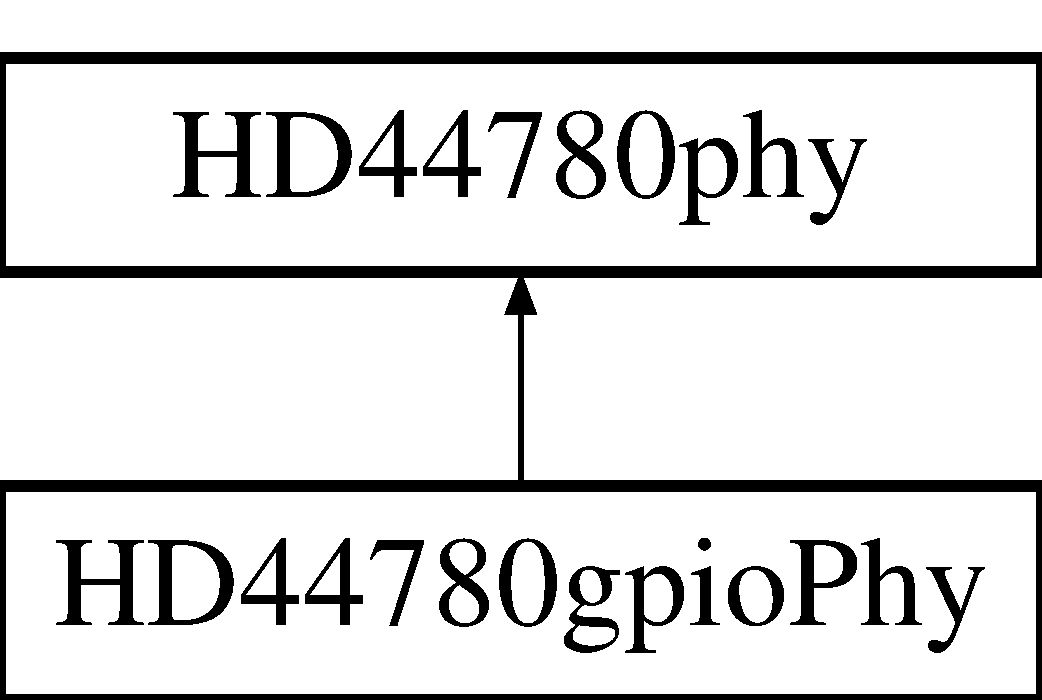
\includegraphics[height=2.000000cm]{class_h_d44780gpio_phy}
\end{center}
\end{figure}
\subsection*{Public Member Functions}
\begin{DoxyCompactItemize}
\item 
\hyperlink{class_h_d44780gpio_phy_a47de0045a7ef81a41c9887ad47c3122f}{H\-D44780gpio\-Phy} (\hyperlink{class_g_p_i_opin}{G\-P\-I\-Opin} $\ast$wires)
\item 
virtual \hyperlink{class_h_d44780gpio_phy_a646fd32d14debc4d369312495c6e77e8}{$\sim$\-H\-D44780gpio\-Phy} ()
\item 
virtual void \hyperlink{class_h_d44780gpio_phy_a1c8e591c8c4c8287f70a7ba398ebb744}{write} (uint8\-\_\-t n, uint8\-\_\-t x)
\begin{DoxyCompactList}\small\item\em Method writes byte v to the display. Method writes byte v to the n-\/th chip on the display. It must implement all operations necessary to write the data. If the display uses 4bit interface, the method must split the value into nibbles and write them in correct order. \end{DoxyCompactList}\item 
virtual uint8\-\_\-t \hyperlink{class_h_d44780gpio_phy_a0a30a28c612d067c3023c4fb5f1388a0}{read} (uint8\-\_\-t n)
\begin{DoxyCompactList}\small\item\em Method reads the data from the display Method reads the data lines from the the n-\/th chip on the display. Register read by the method is selected by the R\-S line. If the hardware interface does not support reading from the display, value returned by the read function is not determined. Ability to read from the display should be tested with {\itshape support\-Read()}. \end{DoxyCompactList}\item 
virtual bool \hyperlink{class_h_d44780gpio_phy_aca1ef4ea05900362e4feb63f062d0b3e}{busy} (uint8\-\_\-t n)
\begin{DoxyCompactList}\small\item\em Method checks status of B\-U\-S\-Y flag If the implementation does not support readback, method should always return false;. \end{DoxyCompactList}\item 
virtual bool \hyperlink{class_h_d44780gpio_phy_a9c2ca3dca1582a529ef154e492ed214a}{supports\-Read} ()
\begin{DoxyCompactList}\small\item\em Method reports status of support for reading from the display. Method should return true if the higher level implementation can relay on reading from the display (e.\-g. status checking v.\-s. delays between operations. \end{DoxyCompactList}\item 
virtual uint8\-\_\-t \hyperlink{class_h_d44780gpio_phy_a933e313ac7a5362b6a55a3db9af337a3}{current\-Data\-Address} (uint8\-\_\-t n)
\begin{DoxyCompactList}\small\item\em Method reads value of the internal. \end{DoxyCompactList}\item 
virtual void \hyperlink{class_h_d44780gpio_phy_a58958f3a1c2e702da568aac6c4c8c32f}{set\-E} (uint8\-\_\-t num, uint8\-\_\-t v)
\begin{DoxyCompactList}\small\item\em Function sets selected E line to requested state. Function sets selected E line to requested state. Selection of enable line allows to support big displays with more than one controllers on board. Enable lines are numbered staring from 0. Value of {\itshape num} can not be ignored. If the hardware interface uses only one enable line, the method should respond only to num set to 0. \end{DoxyCompactList}\item 
virtual void \hyperlink{class_h_d44780gpio_phy_ae396a22b3a46bd163a4b65b1eeb007af}{set\-R\-S} (uint8\-\_\-t v)
\begin{DoxyCompactList}\small\item\em Method sets status of R\-S line. Method sets status of R\-S line selecting instruction (for write), status (for read) registers or data memory (R/\-W). Data\-: R\-S = 1 Instruction\-: R\-S = 0. \end{DoxyCompactList}\item 
virtual void \hyperlink{class_h_d44780gpio_phy_a5465139b8680c044b1ef1a040027f2d3}{set\-R\-W} (uint8\-\_\-t v)
\begin{DoxyCompactList}\small\item\em Method sets status of R\-W line. Method sets status of R\-W line. If the hardware interface does not support readback, this method can be empty. Read\-: R\-W=1 Write\-: R\-W=0. \end{DoxyCompactList}\end{DoxyCompactItemize}
\subsection*{Additional Inherited Members}


\subsection{Detailed Description}
Implementation of physical interface to text displays based on \hyperlink{class_h_d44780}{H\-D44780}, using \hyperlink{class_g_p_i_ooo}{G\-P\-I\-Ooo}. Displays with up to 8 chips are supported. 

\subsection{Constructor \& Destructor Documentation}
\hypertarget{class_h_d44780gpio_phy_a47de0045a7ef81a41c9887ad47c3122f}{\index{H\-D44780gpio\-Phy@{H\-D44780gpio\-Phy}!H\-D44780gpio\-Phy@{H\-D44780gpio\-Phy}}
\index{H\-D44780gpio\-Phy@{H\-D44780gpio\-Phy}!HD44780gpioPhy@{H\-D44780gpio\-Phy}}
\subsubsection[{H\-D44780gpio\-Phy}]{\setlength{\rightskip}{0pt plus 5cm}H\-D44780gpio\-Phy\-::\-H\-D44780gpio\-Phy (
\begin{DoxyParamCaption}
\item[{{\bf G\-P\-I\-Opin} $\ast$}]{wires}
\end{DoxyParamCaption}
)}}\label{class_h_d44780gpio_phy_a47de0045a7ef81a41c9887ad47c3122f}
Constructor initializes interface to text display based on \hyperlink{class_h_d44780}{H\-D44780}. The display is controlled by named G\-P\-I\-O lines from the  wires block. The class supports 4 and 8 bit interfaces. Width of the interface is determined by the number of data lines in the block. Implementation supports multiple chips on the display board. Chips are selected by lines from a block of E\-N\-A\-B\-L\-E lines.

Wires in the G\-P\-I\-O block are identified by their names\-:


\begin{DoxyItemize}
\item D\mbox{[}0\mbox{]} ... D\mbox{[}7\mbox{]} -\/ for data wires. Width of the bus is determined by the number of data wires defined in the block. If 8 wires are present, 8 bit interface will be used. Otherwise if 4 or more wires are present 4-\/bit interface will be used.
\item R\-S -\/ for wire controlling R\-S line
\item R\-W -\/ for wire controlling R/\-W line
\item E -\/ for enable wire if only one chip is present (alternative for E\mbox{[}0\mbox{]})
\item E\mbox{[}0\mbox{]} ... E\mbox{[}7\mbox{]} for Enable wires. Number of chips is determined by the finding the index of first non-\/defined E\mbox{[}x\mbox{]} label. For a set of enable wires (E\mbox{[}0\mbox{]}, E\mbox{[}1\mbox{]}, E\mbox{[}3\mbox{]}) number of chips will be 2, because wire E\mbox{[}2\mbox{]} is not defined. If wire \char`\"{}\-E\char`\"{} is found, wires E\mbox{[}x\mbox{]} will be ignored and only one chip will be supported.
\end{DoxyItemize}

For multi-\/wire buses the names consist of the bus symbol (D for data, E for enable), opening square bracket, one digit of wire index and closing square bracket.


\begin{DoxyParams}{Parameters}
{\em wires} & -\/ block of G\-P\-I\-Os intefacing the display. \\
\hline
\end{DoxyParams}
\hypertarget{class_h_d44780gpio_phy_a646fd32d14debc4d369312495c6e77e8}{\index{H\-D44780gpio\-Phy@{H\-D44780gpio\-Phy}!$\sim$\-H\-D44780gpio\-Phy@{$\sim$\-H\-D44780gpio\-Phy}}
\index{$\sim$\-H\-D44780gpio\-Phy@{$\sim$\-H\-D44780gpio\-Phy}!HD44780gpioPhy@{H\-D44780gpio\-Phy}}
\subsubsection[{$\sim$\-H\-D44780gpio\-Phy}]{\setlength{\rightskip}{0pt plus 5cm}H\-D44780gpio\-Phy\-::$\sim$\-H\-D44780gpio\-Phy (
\begin{DoxyParamCaption}
{}
\end{DoxyParamCaption}
)\hspace{0.3cm}{\ttfamily [virtual]}}}\label{class_h_d44780gpio_phy_a646fd32d14debc4d369312495c6e77e8}


\subsection{Member Function Documentation}
\hypertarget{class_h_d44780gpio_phy_aca1ef4ea05900362e4feb63f062d0b3e}{\index{H\-D44780gpio\-Phy@{H\-D44780gpio\-Phy}!busy@{busy}}
\index{busy@{busy}!HD44780gpioPhy@{H\-D44780gpio\-Phy}}
\subsubsection[{busy}]{\setlength{\rightskip}{0pt plus 5cm}bool H\-D44780gpio\-Phy\-::busy (
\begin{DoxyParamCaption}
\item[{uint8\-\_\-t}]{n}
\end{DoxyParamCaption}
)\hspace{0.3cm}{\ttfamily [virtual]}}}\label{class_h_d44780gpio_phy_aca1ef4ea05900362e4feb63f062d0b3e}


Method checks status of B\-U\-S\-Y flag If the implementation does not support readback, method should always return false;. 

D\-N\-I


\begin{DoxyParams}{Parameters}
{\em n} & -\/ index of the chip on the display \\
\hline
\end{DoxyParams}
\begin{DoxyReturn}{Returns}
true if the display reports B\-U\-S\-Y state. False if the display is busy performing internal operations or readback is not supported. 
\end{DoxyReturn}


Implements \hyperlink{class_h_d44780phy_ab3f91533a8063062dec767d524d704b1}{H\-D44780phy}.

\hypertarget{class_h_d44780gpio_phy_a933e313ac7a5362b6a55a3db9af337a3}{\index{H\-D44780gpio\-Phy@{H\-D44780gpio\-Phy}!current\-Data\-Address@{current\-Data\-Address}}
\index{current\-Data\-Address@{current\-Data\-Address}!HD44780gpioPhy@{H\-D44780gpio\-Phy}}
\subsubsection[{current\-Data\-Address}]{\setlength{\rightskip}{0pt plus 5cm}uint8\-\_\-t H\-D44780gpio\-Phy\-::current\-Data\-Address (
\begin{DoxyParamCaption}
\item[{uint8\-\_\-t}]{n}
\end{DoxyParamCaption}
)\hspace{0.3cm}{\ttfamily [virtual]}}}\label{class_h_d44780gpio_phy_a933e313ac7a5362b6a55a3db9af337a3}


Method reads value of the internal. 

\begin{DoxyReturn}{Returns}

\end{DoxyReturn}


Implements \hyperlink{class_h_d44780phy_a0e848e19d8a5c2c9605b7bf6bcc5394c}{H\-D44780phy}.

\hypertarget{class_h_d44780gpio_phy_a0a30a28c612d067c3023c4fb5f1388a0}{\index{H\-D44780gpio\-Phy@{H\-D44780gpio\-Phy}!read@{read}}
\index{read@{read}!HD44780gpioPhy@{H\-D44780gpio\-Phy}}
\subsubsection[{read}]{\setlength{\rightskip}{0pt plus 5cm}uint8\-\_\-t H\-D44780gpio\-Phy\-::read (
\begin{DoxyParamCaption}
\item[{uint8\-\_\-t}]{n}
\end{DoxyParamCaption}
)\hspace{0.3cm}{\ttfamily [virtual]}}}\label{class_h_d44780gpio_phy_a0a30a28c612d067c3023c4fb5f1388a0}


Method reads the data from the display Method reads the data lines from the the n-\/th chip on the display. Register read by the method is selected by the R\-S line. If the hardware interface does not support reading from the display, value returned by the read function is not determined. Ability to read from the display should be tested with {\itshape support\-Read()}. 


\begin{DoxyParams}{Parameters}
{\em n} & -\/ index of the chip on the display \\
\hline
\end{DoxyParams}
\begin{DoxyReturn}{Returns}
value read from the display. 
\end{DoxyReturn}


Implements \hyperlink{class_h_d44780phy_abdee2bf5155e9915c9bb47b948edd7e1}{H\-D44780phy}.

\hypertarget{class_h_d44780gpio_phy_a58958f3a1c2e702da568aac6c4c8c32f}{\index{H\-D44780gpio\-Phy@{H\-D44780gpio\-Phy}!set\-E@{set\-E}}
\index{set\-E@{set\-E}!HD44780gpioPhy@{H\-D44780gpio\-Phy}}
\subsubsection[{set\-E}]{\setlength{\rightskip}{0pt plus 5cm}void H\-D44780gpio\-Phy\-::set\-E (
\begin{DoxyParamCaption}
\item[{uint8\-\_\-t}]{num, }
\item[{uint8\-\_\-t}]{v}
\end{DoxyParamCaption}
)\hspace{0.3cm}{\ttfamily [virtual]}}}\label{class_h_d44780gpio_phy_a58958f3a1c2e702da568aac6c4c8c32f}


Function sets selected E line to requested state. Function sets selected E line to requested state. Selection of enable line allows to support big displays with more than one controllers on board. Enable lines are numbered staring from 0. Value of {\itshape num} can not be ignored. If the hardware interface uses only one enable line, the method should respond only to num set to 0. 


\begin{DoxyParams}{Parameters}
{\em num} & Index of E line. \\
\hline
{\em v} & Status of E line. \\
\hline
\end{DoxyParams}


Implements \hyperlink{class_h_d44780phy_aa6ec16b9e1ca1400b0c20815d1dd1938}{H\-D44780phy}.

\hypertarget{class_h_d44780gpio_phy_ae396a22b3a46bd163a4b65b1eeb007af}{\index{H\-D44780gpio\-Phy@{H\-D44780gpio\-Phy}!set\-R\-S@{set\-R\-S}}
\index{set\-R\-S@{set\-R\-S}!HD44780gpioPhy@{H\-D44780gpio\-Phy}}
\subsubsection[{set\-R\-S}]{\setlength{\rightskip}{0pt plus 5cm}void H\-D44780gpio\-Phy\-::set\-R\-S (
\begin{DoxyParamCaption}
\item[{uint8\-\_\-t}]{v}
\end{DoxyParamCaption}
)\hspace{0.3cm}{\ttfamily [virtual]}}}\label{class_h_d44780gpio_phy_ae396a22b3a46bd163a4b65b1eeb007af}


Method sets status of R\-S line. Method sets status of R\-S line selecting instruction (for write), status (for read) registers or data memory (R/\-W). Data\-: R\-S = 1 Instruction\-: R\-S = 0. 


\begin{DoxyParams}{Parameters}
{\em v} & requested status of R\-S line. \\
\hline
\end{DoxyParams}


Implements \hyperlink{class_h_d44780phy_a982aed1944e85dcabd0702af526ab2fe}{H\-D44780phy}.

\hypertarget{class_h_d44780gpio_phy_a5465139b8680c044b1ef1a040027f2d3}{\index{H\-D44780gpio\-Phy@{H\-D44780gpio\-Phy}!set\-R\-W@{set\-R\-W}}
\index{set\-R\-W@{set\-R\-W}!HD44780gpioPhy@{H\-D44780gpio\-Phy}}
\subsubsection[{set\-R\-W}]{\setlength{\rightskip}{0pt plus 5cm}void H\-D44780gpio\-Phy\-::set\-R\-W (
\begin{DoxyParamCaption}
\item[{uint8\-\_\-t}]{v}
\end{DoxyParamCaption}
)\hspace{0.3cm}{\ttfamily [virtual]}}}\label{class_h_d44780gpio_phy_a5465139b8680c044b1ef1a040027f2d3}


Method sets status of R\-W line. Method sets status of R\-W line. If the hardware interface does not support readback, this method can be empty. Read\-: R\-W=1 Write\-: R\-W=0. 


\begin{DoxyParams}{Parameters}
{\em v} & requested status of R\-S line. \\
\hline
\end{DoxyParams}


Implements \hyperlink{class_h_d44780phy_a2885ef9168fc5a6c73233f8c7e9ed404}{H\-D44780phy}.

\hypertarget{class_h_d44780gpio_phy_a9c2ca3dca1582a529ef154e492ed214a}{\index{H\-D44780gpio\-Phy@{H\-D44780gpio\-Phy}!supports\-Read@{supports\-Read}}
\index{supports\-Read@{supports\-Read}!HD44780gpioPhy@{H\-D44780gpio\-Phy}}
\subsubsection[{supports\-Read}]{\setlength{\rightskip}{0pt plus 5cm}virtual bool H\-D44780gpio\-Phy\-::supports\-Read (
\begin{DoxyParamCaption}
{}
\end{DoxyParamCaption}
)\hspace{0.3cm}{\ttfamily [inline]}, {\ttfamily [virtual]}}}\label{class_h_d44780gpio_phy_a9c2ca3dca1582a529ef154e492ed214a}


Method reports status of support for reading from the display. Method should return true if the higher level implementation can relay on reading from the display (e.\-g. status checking v.\-s. delays between operations. 

\begin{DoxyReturn}{Returns}
true of reading B\-U\-S\-Y flag is supported. 
\end{DoxyReturn}


Implements \hyperlink{class_h_d44780phy_ad3caa3cc36f03230ed9c209bb576a050}{H\-D44780phy}.

\hypertarget{class_h_d44780gpio_phy_a1c8e591c8c4c8287f70a7ba398ebb744}{\index{H\-D44780gpio\-Phy@{H\-D44780gpio\-Phy}!write@{write}}
\index{write@{write}!HD44780gpioPhy@{H\-D44780gpio\-Phy}}
\subsubsection[{write}]{\setlength{\rightskip}{0pt plus 5cm}void H\-D44780gpio\-Phy\-::write (
\begin{DoxyParamCaption}
\item[{uint8\-\_\-t}]{n, }
\item[{uint8\-\_\-t}]{x}
\end{DoxyParamCaption}
)\hspace{0.3cm}{\ttfamily [virtual]}}}\label{class_h_d44780gpio_phy_a1c8e591c8c4c8287f70a7ba398ebb744}


Method writes byte v to the display. Method writes byte v to the n-\/th chip on the display. It must implement all operations necessary to write the data. If the display uses 4bit interface, the method must split the value into nibbles and write them in correct order. 


\begin{DoxyParams}{Parameters}
{\em n} & -\/ index of the chip on the display \\
\hline
{\em x} & value to be written \\
\hline
\end{DoxyParams}


Implements \hyperlink{class_h_d44780phy_a279090fa11ae5dffd881b62ed972637b}{H\-D44780phy}.



The documentation for this class was generated from the following files\-:\begin{DoxyCompactItemize}
\item 
include/device/\hyperlink{_h_d44780gpio_phy_8h}{H\-D44780gpio\-Phy.\-h}\item 
src/\hyperlink{_h_d44780gpio_phy_8cpp}{H\-D44780gpio\-Phy.\-cpp}\end{DoxyCompactItemize}

\hypertarget{class_h_d44780phy}{\section{H\-D44780phy Class Reference}
\label{class_h_d44780phy}\index{H\-D44780phy@{H\-D44780phy}}
}


{\ttfamily \#include $<$H\-D44780phy.\-h$>$}

Inheritance diagram for H\-D44780phy\-:\begin{figure}[H]
\begin{center}
\leavevmode
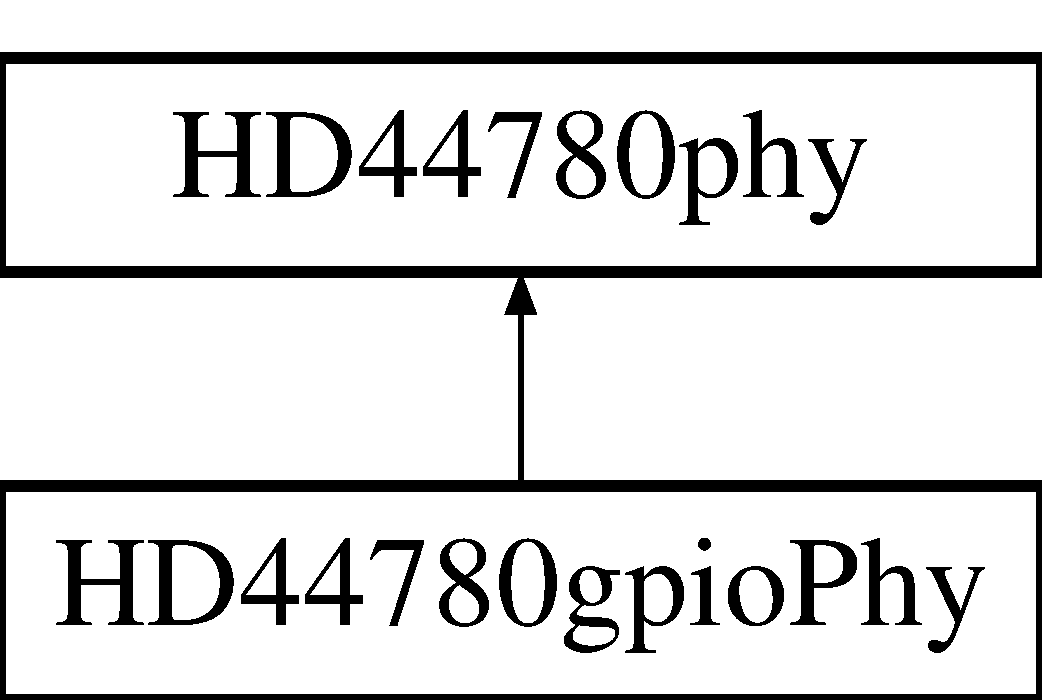
\includegraphics[height=2.000000cm]{class_h_d44780phy}
\end{center}
\end{figure}
\subsection*{Public Types}
\begin{DoxyCompactItemize}
\item 
enum \{ \hyperlink{class_h_d44780phy_a76851a61a3a88766704db9f31098d21fac3d8b04a4b6fa7db3d0bfc61170e1d72}{R\-Scommand} = 0, 
\hyperlink{class_h_d44780phy_a76851a61a3a88766704db9f31098d21fa2108dbcf0cc7b6cdcbc6235a4e765654}{R\-Sdata} = 1
 \}
\item 
enum \{ \hyperlink{class_h_d44780phy_a5bf3a330184d4cfdc6297c1265ce6746ac7b87f6864ebbc4bef3d14967ec3bc97}{R\-Wwrite} = 0, 
\hyperlink{class_h_d44780phy_a5bf3a330184d4cfdc6297c1265ce6746a2777116400417dda3d881ec137a361fc}{R\-Wread} = 1
 \}
\end{DoxyCompactItemize}
\subsection*{Public Member Functions}
\begin{DoxyCompactItemize}
\item 
\hyperlink{class_h_d44780phy_a1e285c5a059e498acbd65d411ca7cb4d}{H\-D44780phy} ()
\item 
virtual \hyperlink{class_h_d44780phy_a7ec413f9bde27b85f43554b1cdc4860a}{$\sim$\-H\-D44780phy} ()
\item 
virtual void \hyperlink{class_h_d44780phy_a279090fa11ae5dffd881b62ed972637b}{write} (uint8\-\_\-t n, uint8\-\_\-t x)=0
\begin{DoxyCompactList}\small\item\em Method writes byte v to the display. Method writes byte v to the n-\/th chip on the display. It must implement all operations necessary to write the data. If the display uses 4bit interface, the method must split the value into nibbles and write them in correct order. \end{DoxyCompactList}\item 
virtual bool \hyperlink{class_h_d44780phy_ad3caa3cc36f03230ed9c209bb576a050}{supports\-Read} ()=0
\begin{DoxyCompactList}\small\item\em Method reports status of support for reading from the display. Method should return true if the higher level implementation can relay on reading from the display (e.\-g. status checking v.\-s. delays between operations. \end{DoxyCompactList}\item 
virtual uint8\-\_\-t \hyperlink{class_h_d44780phy_abdee2bf5155e9915c9bb47b948edd7e1}{read} (uint8\-\_\-t n)=0
\begin{DoxyCompactList}\small\item\em Method reads the data from the display Method reads the data lines from the the n-\/th chip on the display. Register read by the method is selected by the R\-S line. If the hardware interface does not support reading from the display, value returned by the read function is not determined. Ability to read from the display should be tested with {\itshape support\-Read()}. \end{DoxyCompactList}\item 
virtual bool \hyperlink{class_h_d44780phy_ab3f91533a8063062dec767d524d704b1}{busy} (uint8\-\_\-t n)=0
\begin{DoxyCompactList}\small\item\em Method checks status of B\-U\-S\-Y flag If the implementation does not support readback, method should always return false;. \end{DoxyCompactList}\item 
virtual uint8\-\_\-t \hyperlink{class_h_d44780phy_a0e848e19d8a5c2c9605b7bf6bcc5394c}{current\-Data\-Address} (uint8\-\_\-t n)=0
\begin{DoxyCompactList}\small\item\em Method reads value of the internal. \end{DoxyCompactList}\item 
virtual void \hyperlink{class_h_d44780phy_aa6ec16b9e1ca1400b0c20815d1dd1938}{set\-E} (uint8\-\_\-t num, uint8\-\_\-t v)=0
\begin{DoxyCompactList}\small\item\em Function sets selected E line to requested state. Function sets selected E line to requested state. Selection of enable line allows to support big displays with more than one controllers on board. Enable lines are numbered staring from 0. Value of {\itshape num} can not be ignored. If the hardware interface uses only one enable line, the method should respond only to num set to 0. \end{DoxyCompactList}\item 
virtual void \hyperlink{class_h_d44780phy_a982aed1944e85dcabd0702af526ab2fe}{set\-R\-S} (uint8\-\_\-t v)=0
\begin{DoxyCompactList}\small\item\em Method sets status of R\-S line. Method sets status of R\-S line selecting instruction (for write), status (for read) registers or data memory (R/\-W). Data\-: R\-S = 1 Instruction\-: R\-S = 0. \end{DoxyCompactList}\item 
virtual void \hyperlink{class_h_d44780phy_a2885ef9168fc5a6c73233f8c7e9ed404}{set\-R\-W} (uint8\-\_\-t v)=0
\begin{DoxyCompactList}\small\item\em Method sets status of R\-W line. Method sets status of R\-W line. If the hardware interface does not support readback, this method can be empty. Read\-: R\-W=1 Write\-: R\-W=0. \end{DoxyCompactList}\item 
int \hyperlink{class_h_d44780phy_a621aad1a63c6fe9f061c0914c6afefe9}{get\-Bits} () const 
\end{DoxyCompactItemize}
\subsection*{Protected Attributes}
\begin{DoxyCompactItemize}
\item 
int \hyperlink{class_h_d44780phy_aa50b8a72c2a3418cda74b4693e8e1253}{bits}
\end{DoxyCompactItemize}


\subsection{Detailed Description}
Class defines interface to the display. Higher level functions use the interface for low level communication. Implementation of the interface should support 8 or 4 bit communication (depending on hardware implementation), exposing to the higher layer only 8-\/bit interface. The implementation must honor multiple chip select (enable) lines, for displays with multiple \hyperlink{class_h_d44780}{H\-D44780} chips on board. All requests to chips with indexes beyond the number of supported enable lines should be ignored.

The class should not be use to drive multiple displays connected to the data and control bus, unless they are supposed to act as one composite display. To drive multiple independent displays sharing data and control bus each display, each display should have a separate instance of \hyperlink{class_h_d44780phy}{H\-D44780phy} object, controlled by separate blocks of I\-O lines sharing the data and control lines, with different enable lines. 

\subsection{Member Enumeration Documentation}
\hypertarget{class_h_d44780phy_a76851a61a3a88766704db9f31098d21f}{\subsubsection[{anonymous enum}]{\setlength{\rightskip}{0pt plus 5cm}anonymous enum}}\label{class_h_d44780phy_a76851a61a3a88766704db9f31098d21f}
Constants for set\-R\-S \begin{Desc}
\item[Enumerator\-: ]\par
\begin{description}
\index{R\-Scommand@{R\-Scommand}!H\-D44780phy@{H\-D44780phy}}\index{H\-D44780phy@{H\-D44780phy}!R\-Scommand@{R\-Scommand}}\item[{\em 
\hypertarget{class_h_d44780phy_a76851a61a3a88766704db9f31098d21fac3d8b04a4b6fa7db3d0bfc61170e1d72}{R\-Scommand}\label{class_h_d44780phy_a76851a61a3a88766704db9f31098d21fac3d8b04a4b6fa7db3d0bfc61170e1d72}
}]R\-Scommand -\/ sets command mode. \index{R\-Sdata@{R\-Sdata}!H\-D44780phy@{H\-D44780phy}}\index{H\-D44780phy@{H\-D44780phy}!R\-Sdata@{R\-Sdata}}\item[{\em 
\hypertarget{class_h_d44780phy_a76851a61a3a88766704db9f31098d21fa2108dbcf0cc7b6cdcbc6235a4e765654}{R\-Sdata}\label{class_h_d44780phy_a76851a61a3a88766704db9f31098d21fa2108dbcf0cc7b6cdcbc6235a4e765654}
}]R\-Sdata -\/ sets data mode. \end{description}
\end{Desc}

\hypertarget{class_h_d44780phy_a5bf3a330184d4cfdc6297c1265ce6746}{\subsubsection[{anonymous enum}]{\setlength{\rightskip}{0pt plus 5cm}anonymous enum}}\label{class_h_d44780phy_a5bf3a330184d4cfdc6297c1265ce6746}
constants for set\-R\-W \begin{Desc}
\item[Enumerator\-: ]\par
\begin{description}
\index{R\-Wwrite@{R\-Wwrite}!H\-D44780phy@{H\-D44780phy}}\index{H\-D44780phy@{H\-D44780phy}!R\-Wwrite@{R\-Wwrite}}\item[{\em 
\hypertarget{class_h_d44780phy_a5bf3a330184d4cfdc6297c1265ce6746ac7b87f6864ebbc4bef3d14967ec3bc97}{R\-Wwrite}\label{class_h_d44780phy_a5bf3a330184d4cfdc6297c1265ce6746ac7b87f6864ebbc4bef3d14967ec3bc97}
}]R\-Wwrite -\/ sets write mode. \index{R\-Wread@{R\-Wread}!H\-D44780phy@{H\-D44780phy}}\index{H\-D44780phy@{H\-D44780phy}!R\-Wread@{R\-Wread}}\item[{\em 
\hypertarget{class_h_d44780phy_a5bf3a330184d4cfdc6297c1265ce6746a2777116400417dda3d881ec137a361fc}{R\-Wread}\label{class_h_d44780phy_a5bf3a330184d4cfdc6297c1265ce6746a2777116400417dda3d881ec137a361fc}
}]R\-Wread -\/ sets read mode. \end{description}
\end{Desc}



\subsection{Constructor \& Destructor Documentation}
\hypertarget{class_h_d44780phy_a1e285c5a059e498acbd65d411ca7cb4d}{\index{H\-D44780phy@{H\-D44780phy}!H\-D44780phy@{H\-D44780phy}}
\index{H\-D44780phy@{H\-D44780phy}!HD44780phy@{H\-D44780phy}}
\subsubsection[{H\-D44780phy}]{\setlength{\rightskip}{0pt plus 5cm}H\-D44780phy\-::\-H\-D44780phy (
\begin{DoxyParamCaption}
{}
\end{DoxyParamCaption}
)\hspace{0.3cm}{\ttfamily [inline]}}}\label{class_h_d44780phy_a1e285c5a059e498acbd65d411ca7cb4d}
\hypertarget{class_h_d44780phy_a7ec413f9bde27b85f43554b1cdc4860a}{\index{H\-D44780phy@{H\-D44780phy}!$\sim$\-H\-D44780phy@{$\sim$\-H\-D44780phy}}
\index{$\sim$\-H\-D44780phy@{$\sim$\-H\-D44780phy}!HD44780phy@{H\-D44780phy}}
\subsubsection[{$\sim$\-H\-D44780phy}]{\setlength{\rightskip}{0pt plus 5cm}virtual H\-D44780phy\-::$\sim$\-H\-D44780phy (
\begin{DoxyParamCaption}
{}
\end{DoxyParamCaption}
)\hspace{0.3cm}{\ttfamily [inline]}, {\ttfamily [virtual]}}}\label{class_h_d44780phy_a7ec413f9bde27b85f43554b1cdc4860a}


\subsection{Member Function Documentation}
\hypertarget{class_h_d44780phy_ab3f91533a8063062dec767d524d704b1}{\index{H\-D44780phy@{H\-D44780phy}!busy@{busy}}
\index{busy@{busy}!HD44780phy@{H\-D44780phy}}
\subsubsection[{busy}]{\setlength{\rightskip}{0pt plus 5cm}virtual bool H\-D44780phy\-::busy (
\begin{DoxyParamCaption}
\item[{uint8\-\_\-t}]{n}
\end{DoxyParamCaption}
)\hspace{0.3cm}{\ttfamily [pure virtual]}}}\label{class_h_d44780phy_ab3f91533a8063062dec767d524d704b1}


Method checks status of B\-U\-S\-Y flag If the implementation does not support readback, method should always return false;. 

D\-N\-I


\begin{DoxyParams}{Parameters}
{\em n} & -\/ index of the chip on the display \\
\hline
\end{DoxyParams}
\begin{DoxyReturn}{Returns}
true if the display reports B\-U\-S\-Y state. False if the display is busy performing internal operations or readback is not supported. 
\end{DoxyReturn}


Implemented in \hyperlink{class_h_d44780gpio_phy_aca1ef4ea05900362e4feb63f062d0b3e}{H\-D44780gpio\-Phy}.

\hypertarget{class_h_d44780phy_a0e848e19d8a5c2c9605b7bf6bcc5394c}{\index{H\-D44780phy@{H\-D44780phy}!current\-Data\-Address@{current\-Data\-Address}}
\index{current\-Data\-Address@{current\-Data\-Address}!HD44780phy@{H\-D44780phy}}
\subsubsection[{current\-Data\-Address}]{\setlength{\rightskip}{0pt plus 5cm}virtual uint8\-\_\-t H\-D44780phy\-::current\-Data\-Address (
\begin{DoxyParamCaption}
\item[{uint8\-\_\-t}]{n}
\end{DoxyParamCaption}
)\hspace{0.3cm}{\ttfamily [pure virtual]}}}\label{class_h_d44780phy_a0e848e19d8a5c2c9605b7bf6bcc5394c}


Method reads value of the internal. 

\begin{DoxyReturn}{Returns}

\end{DoxyReturn}


Implemented in \hyperlink{class_h_d44780gpio_phy_a933e313ac7a5362b6a55a3db9af337a3}{H\-D44780gpio\-Phy}.

\hypertarget{class_h_d44780phy_a621aad1a63c6fe9f061c0914c6afefe9}{\index{H\-D44780phy@{H\-D44780phy}!get\-Bits@{get\-Bits}}
\index{get\-Bits@{get\-Bits}!HD44780phy@{H\-D44780phy}}
\subsubsection[{get\-Bits}]{\setlength{\rightskip}{0pt plus 5cm}int H\-D44780phy\-::get\-Bits (
\begin{DoxyParamCaption}
{}
\end{DoxyParamCaption}
) const\hspace{0.3cm}{\ttfamily [inline]}}}\label{class_h_d44780phy_a621aad1a63c6fe9f061c0914c6afefe9}
\hypertarget{class_h_d44780phy_abdee2bf5155e9915c9bb47b948edd7e1}{\index{H\-D44780phy@{H\-D44780phy}!read@{read}}
\index{read@{read}!HD44780phy@{H\-D44780phy}}
\subsubsection[{read}]{\setlength{\rightskip}{0pt plus 5cm}virtual uint8\-\_\-t H\-D44780phy\-::read (
\begin{DoxyParamCaption}
\item[{uint8\-\_\-t}]{n}
\end{DoxyParamCaption}
)\hspace{0.3cm}{\ttfamily [pure virtual]}}}\label{class_h_d44780phy_abdee2bf5155e9915c9bb47b948edd7e1}


Method reads the data from the display Method reads the data lines from the the n-\/th chip on the display. Register read by the method is selected by the R\-S line. If the hardware interface does not support reading from the display, value returned by the read function is not determined. Ability to read from the display should be tested with {\itshape support\-Read()}. 


\begin{DoxyParams}{Parameters}
{\em n} & -\/ index of the chip on the display \\
\hline
\end{DoxyParams}
\begin{DoxyReturn}{Returns}
value read from the display. 
\end{DoxyReturn}


Implemented in \hyperlink{class_h_d44780gpio_phy_a0a30a28c612d067c3023c4fb5f1388a0}{H\-D44780gpio\-Phy}.

\hypertarget{class_h_d44780phy_aa6ec16b9e1ca1400b0c20815d1dd1938}{\index{H\-D44780phy@{H\-D44780phy}!set\-E@{set\-E}}
\index{set\-E@{set\-E}!HD44780phy@{H\-D44780phy}}
\subsubsection[{set\-E}]{\setlength{\rightskip}{0pt plus 5cm}virtual void H\-D44780phy\-::set\-E (
\begin{DoxyParamCaption}
\item[{uint8\-\_\-t}]{num, }
\item[{uint8\-\_\-t}]{v}
\end{DoxyParamCaption}
)\hspace{0.3cm}{\ttfamily [pure virtual]}}}\label{class_h_d44780phy_aa6ec16b9e1ca1400b0c20815d1dd1938}


Function sets selected E line to requested state. Function sets selected E line to requested state. Selection of enable line allows to support big displays with more than one controllers on board. Enable lines are numbered staring from 0. Value of {\itshape num} can not be ignored. If the hardware interface uses only one enable line, the method should respond only to num set to 0. 


\begin{DoxyParams}{Parameters}
{\em num} & Index of E line. \\
\hline
{\em v} & Status of E line. \\
\hline
\end{DoxyParams}


Implemented in \hyperlink{class_h_d44780gpio_phy_a58958f3a1c2e702da568aac6c4c8c32f}{H\-D44780gpio\-Phy}.

\hypertarget{class_h_d44780phy_a982aed1944e85dcabd0702af526ab2fe}{\index{H\-D44780phy@{H\-D44780phy}!set\-R\-S@{set\-R\-S}}
\index{set\-R\-S@{set\-R\-S}!HD44780phy@{H\-D44780phy}}
\subsubsection[{set\-R\-S}]{\setlength{\rightskip}{0pt plus 5cm}virtual void H\-D44780phy\-::set\-R\-S (
\begin{DoxyParamCaption}
\item[{uint8\-\_\-t}]{v}
\end{DoxyParamCaption}
)\hspace{0.3cm}{\ttfamily [pure virtual]}}}\label{class_h_d44780phy_a982aed1944e85dcabd0702af526ab2fe}


Method sets status of R\-S line. Method sets status of R\-S line selecting instruction (for write), status (for read) registers or data memory (R/\-W). Data\-: R\-S = 1 Instruction\-: R\-S = 0. 


\begin{DoxyParams}{Parameters}
{\em v} & requested status of R\-S line. \\
\hline
\end{DoxyParams}


Implemented in \hyperlink{class_h_d44780gpio_phy_ae396a22b3a46bd163a4b65b1eeb007af}{H\-D44780gpio\-Phy}.

\hypertarget{class_h_d44780phy_a2885ef9168fc5a6c73233f8c7e9ed404}{\index{H\-D44780phy@{H\-D44780phy}!set\-R\-W@{set\-R\-W}}
\index{set\-R\-W@{set\-R\-W}!HD44780phy@{H\-D44780phy}}
\subsubsection[{set\-R\-W}]{\setlength{\rightskip}{0pt plus 5cm}virtual void H\-D44780phy\-::set\-R\-W (
\begin{DoxyParamCaption}
\item[{uint8\-\_\-t}]{v}
\end{DoxyParamCaption}
)\hspace{0.3cm}{\ttfamily [pure virtual]}}}\label{class_h_d44780phy_a2885ef9168fc5a6c73233f8c7e9ed404}


Method sets status of R\-W line. Method sets status of R\-W line. If the hardware interface does not support readback, this method can be empty. Read\-: R\-W=1 Write\-: R\-W=0. 


\begin{DoxyParams}{Parameters}
{\em v} & requested status of R\-S line. \\
\hline
\end{DoxyParams}


Implemented in \hyperlink{class_h_d44780gpio_phy_a5465139b8680c044b1ef1a040027f2d3}{H\-D44780gpio\-Phy}.

\hypertarget{class_h_d44780phy_ad3caa3cc36f03230ed9c209bb576a050}{\index{H\-D44780phy@{H\-D44780phy}!supports\-Read@{supports\-Read}}
\index{supports\-Read@{supports\-Read}!HD44780phy@{H\-D44780phy}}
\subsubsection[{supports\-Read}]{\setlength{\rightskip}{0pt plus 5cm}virtual bool H\-D44780phy\-::supports\-Read (
\begin{DoxyParamCaption}
{}
\end{DoxyParamCaption}
)\hspace{0.3cm}{\ttfamily [pure virtual]}}}\label{class_h_d44780phy_ad3caa3cc36f03230ed9c209bb576a050}


Method reports status of support for reading from the display. Method should return true if the higher level implementation can relay on reading from the display (e.\-g. status checking v.\-s. delays between operations. 

\begin{DoxyReturn}{Returns}
true of reading B\-U\-S\-Y flag is supported. 
\end{DoxyReturn}


Implemented in \hyperlink{class_h_d44780gpio_phy_a9c2ca3dca1582a529ef154e492ed214a}{H\-D44780gpio\-Phy}.

\hypertarget{class_h_d44780phy_a279090fa11ae5dffd881b62ed972637b}{\index{H\-D44780phy@{H\-D44780phy}!write@{write}}
\index{write@{write}!HD44780phy@{H\-D44780phy}}
\subsubsection[{write}]{\setlength{\rightskip}{0pt plus 5cm}virtual void H\-D44780phy\-::write (
\begin{DoxyParamCaption}
\item[{uint8\-\_\-t}]{n, }
\item[{uint8\-\_\-t}]{x}
\end{DoxyParamCaption}
)\hspace{0.3cm}{\ttfamily [pure virtual]}}}\label{class_h_d44780phy_a279090fa11ae5dffd881b62ed972637b}


Method writes byte v to the display. Method writes byte v to the n-\/th chip on the display. It must implement all operations necessary to write the data. If the display uses 4bit interface, the method must split the value into nibbles and write them in correct order. 


\begin{DoxyParams}{Parameters}
{\em n} & -\/ index of the chip on the display \\
\hline
{\em x} & value to be written \\
\hline
\end{DoxyParams}


Implemented in \hyperlink{class_h_d44780gpio_phy_a1c8e591c8c4c8287f70a7ba398ebb744}{H\-D44780gpio\-Phy}.



\subsection{Member Data Documentation}
\hypertarget{class_h_d44780phy_aa50b8a72c2a3418cda74b4693e8e1253}{\index{H\-D44780phy@{H\-D44780phy}!bits@{bits}}
\index{bits@{bits}!HD44780phy@{H\-D44780phy}}
\subsubsection[{bits}]{\setlength{\rightskip}{0pt plus 5cm}int H\-D44780phy\-::bits\hspace{0.3cm}{\ttfamily [protected]}}}\label{class_h_d44780phy_aa50b8a72c2a3418cda74b4693e8e1253}


The documentation for this class was generated from the following file\-:\begin{DoxyCompactItemize}
\item 
include/device/\hyperlink{_h_d44780phy_8h}{H\-D44780phy.\-h}\end{DoxyCompactItemize}

\hypertarget{structpru__data}{\section{pru\-\_\-data Struct Reference}
\label{structpru__data}\index{pru\-\_\-data@{pru\-\_\-data}}
}
\subsection*{Public Attributes}
\begin{DoxyCompactItemize}
\item 
uint8\-\_\-t $\ast$ \hyperlink{structpru__data_a29e00509c51ee8e22747b609333dfe1c}{prumem}
\end{DoxyCompactItemize}


\subsection{Member Data Documentation}
\hypertarget{structpru__data_a29e00509c51ee8e22747b609333dfe1c}{\index{pru\-\_\-data@{pru\-\_\-data}!prumem@{prumem}}
\index{prumem@{prumem}!pru_data@{pru\-\_\-data}}
\subsubsection[{prumem}]{\setlength{\rightskip}{0pt plus 5cm}uint8\-\_\-t$\ast$ pru\-\_\-data\-::prumem}}\label{structpru__data_a29e00509c51ee8e22747b609333dfe1c}


The documentation for this struct was generated from the following file\-:\begin{DoxyCompactItemize}
\item 
examples/\hyperlink{pru__loader_8c}{pru\-\_\-loader.\-c}\end{DoxyCompactItemize}

\hypertarget{class_s_p_i}{\section{S\-P\-I Class Reference}
\label{class_s_p_i}\index{S\-P\-I@{S\-P\-I}}
}


{\ttfamily \#include $<$S\-P\-I.\-h$>$}

\subsection*{Public Member Functions}
\begin{DoxyCompactItemize}
\item 
\hyperlink{class_s_p_i_a2ba081c29fbdecc704c6bf00b24d5205}{S\-P\-I} ()
\item 
int \hyperlink{class_s_p_i_a52ceb41efea8b56cd6c5fc20cd36ca33}{open} (int bus, int channel)
\item 
int \hyperlink{class_s_p_i_ab60d93bf6b639c0b4dad9da4f5854a94}{close} ()
\item 
int \hyperlink{class_s_p_i_a81ff077c6af077ef9d1ee2d56a8a310b}{set\-Mode} (uint8\-\_\-t mode)
\item 
int \hyperlink{class_s_p_i_afad281dadda690a5bb1ad456c2ddb924}{set\-Clock\-Polarity} (uint8\-\_\-t pol)
\item 
int \hyperlink{class_s_p_i_acc43a43a985c6e73723852d621324ef8}{set\-Clock\-Phase} (uint8\-\_\-t phase)
\item 
int \hyperlink{class_s_p_i_aedcab28ad20f691db0f3450ed825fd69}{set\-L\-S\-B\-First} (bool lsb\-\_\-first)
\item 
int \hyperlink{class_s_p_i_a4e6b7a9b89809663c91712ceff00920b}{set\-Bits\-Per\-Word} (int bits)
\item 
int \hyperlink{class_s_p_i_a3de287340d081fc813fd21269b014183}{set\-Speed} (uint32\-\_\-t speed)
\item 
int \hyperlink{class_s_p_i_a7349053056a1e712eb6f5c1f122186d0}{write} (uint8\-\_\-t wbuf\mbox{[}$\,$\mbox{]}, int len)
\item 
int \hyperlink{class_s_p_i_a001a78d9fbd2ea73b0fcb7b5efa816e0}{read} (uint8\-\_\-t rbuf\mbox{[}$\,$\mbox{]}, int len)
\item 
int \hyperlink{class_s_p_i_adcd3b90ca766fb1b69666cf3402726fe}{xfer1} (uint8\-\_\-t wbuf\mbox{[}$\,$\mbox{]}, uint8\-\_\-t rbuf\mbox{[}$\,$\mbox{]}, int len)
\item 
virtual \hyperlink{class_s_p_i_a6babebf1ea3e8ff0330f43a3e2312ac4}{$\sim$\-S\-P\-I} ()
\end{DoxyCompactItemize}


\subsection{Constructor \& Destructor Documentation}
\hypertarget{class_s_p_i_a2ba081c29fbdecc704c6bf00b24d5205}{\index{S\-P\-I@{S\-P\-I}!S\-P\-I@{S\-P\-I}}
\index{S\-P\-I@{S\-P\-I}!SPI@{S\-P\-I}}
\subsubsection[{S\-P\-I}]{\setlength{\rightskip}{0pt plus 5cm}S\-P\-I\-::\-S\-P\-I (
\begin{DoxyParamCaption}
{}
\end{DoxyParamCaption}
)}}\label{class_s_p_i_a2ba081c29fbdecc704c6bf00b24d5205}
\hypertarget{class_s_p_i_a6babebf1ea3e8ff0330f43a3e2312ac4}{\index{S\-P\-I@{S\-P\-I}!$\sim$\-S\-P\-I@{$\sim$\-S\-P\-I}}
\index{$\sim$\-S\-P\-I@{$\sim$\-S\-P\-I}!SPI@{S\-P\-I}}
\subsubsection[{$\sim$\-S\-P\-I}]{\setlength{\rightskip}{0pt plus 5cm}S\-P\-I\-::$\sim$\-S\-P\-I (
\begin{DoxyParamCaption}
{}
\end{DoxyParamCaption}
)\hspace{0.3cm}{\ttfamily [virtual]}}}\label{class_s_p_i_a6babebf1ea3e8ff0330f43a3e2312ac4}


\subsection{Member Function Documentation}
\hypertarget{class_s_p_i_ab60d93bf6b639c0b4dad9da4f5854a94}{\index{S\-P\-I@{S\-P\-I}!close@{close}}
\index{close@{close}!SPI@{S\-P\-I}}
\subsubsection[{close}]{\setlength{\rightskip}{0pt plus 5cm}int S\-P\-I\-::close (
\begin{DoxyParamCaption}
{}
\end{DoxyParamCaption}
)}}\label{class_s_p_i_ab60d93bf6b639c0b4dad9da4f5854a94}
\hypertarget{class_s_p_i_a52ceb41efea8b56cd6c5fc20cd36ca33}{\index{S\-P\-I@{S\-P\-I}!open@{open}}
\index{open@{open}!SPI@{S\-P\-I}}
\subsubsection[{open}]{\setlength{\rightskip}{0pt plus 5cm}int S\-P\-I\-::open (
\begin{DoxyParamCaption}
\item[{int}]{bus, }
\item[{int}]{channel}
\end{DoxyParamCaption}
)}}\label{class_s_p_i_a52ceb41efea8b56cd6c5fc20cd36ca33}
\hypertarget{class_s_p_i_a001a78d9fbd2ea73b0fcb7b5efa816e0}{\index{S\-P\-I@{S\-P\-I}!read@{read}}
\index{read@{read}!SPI@{S\-P\-I}}
\subsubsection[{read}]{\setlength{\rightskip}{0pt plus 5cm}int S\-P\-I\-::read (
\begin{DoxyParamCaption}
\item[{uint8\-\_\-t}]{rbuf\mbox{[}$\,$\mbox{]}, }
\item[{int}]{len}
\end{DoxyParamCaption}
)}}\label{class_s_p_i_a001a78d9fbd2ea73b0fcb7b5efa816e0}
\hypertarget{class_s_p_i_a4e6b7a9b89809663c91712ceff00920b}{\index{S\-P\-I@{S\-P\-I}!set\-Bits\-Per\-Word@{set\-Bits\-Per\-Word}}
\index{set\-Bits\-Per\-Word@{set\-Bits\-Per\-Word}!SPI@{S\-P\-I}}
\subsubsection[{set\-Bits\-Per\-Word}]{\setlength{\rightskip}{0pt plus 5cm}int S\-P\-I\-::set\-Bits\-Per\-Word (
\begin{DoxyParamCaption}
\item[{int}]{bits}
\end{DoxyParamCaption}
)}}\label{class_s_p_i_a4e6b7a9b89809663c91712ceff00920b}
\hypertarget{class_s_p_i_acc43a43a985c6e73723852d621324ef8}{\index{S\-P\-I@{S\-P\-I}!set\-Clock\-Phase@{set\-Clock\-Phase}}
\index{set\-Clock\-Phase@{set\-Clock\-Phase}!SPI@{S\-P\-I}}
\subsubsection[{set\-Clock\-Phase}]{\setlength{\rightskip}{0pt plus 5cm}int S\-P\-I\-::set\-Clock\-Phase (
\begin{DoxyParamCaption}
\item[{uint8\-\_\-t}]{phase}
\end{DoxyParamCaption}
)}}\label{class_s_p_i_acc43a43a985c6e73723852d621324ef8}
\hypertarget{class_s_p_i_afad281dadda690a5bb1ad456c2ddb924}{\index{S\-P\-I@{S\-P\-I}!set\-Clock\-Polarity@{set\-Clock\-Polarity}}
\index{set\-Clock\-Polarity@{set\-Clock\-Polarity}!SPI@{S\-P\-I}}
\subsubsection[{set\-Clock\-Polarity}]{\setlength{\rightskip}{0pt plus 5cm}int S\-P\-I\-::set\-Clock\-Polarity (
\begin{DoxyParamCaption}
\item[{uint8\-\_\-t}]{pol}
\end{DoxyParamCaption}
)}}\label{class_s_p_i_afad281dadda690a5bb1ad456c2ddb924}
\hypertarget{class_s_p_i_aedcab28ad20f691db0f3450ed825fd69}{\index{S\-P\-I@{S\-P\-I}!set\-L\-S\-B\-First@{set\-L\-S\-B\-First}}
\index{set\-L\-S\-B\-First@{set\-L\-S\-B\-First}!SPI@{S\-P\-I}}
\subsubsection[{set\-L\-S\-B\-First}]{\setlength{\rightskip}{0pt plus 5cm}int S\-P\-I\-::set\-L\-S\-B\-First (
\begin{DoxyParamCaption}
\item[{bool}]{lsb\-\_\-first}
\end{DoxyParamCaption}
)}}\label{class_s_p_i_aedcab28ad20f691db0f3450ed825fd69}
\hypertarget{class_s_p_i_a81ff077c6af077ef9d1ee2d56a8a310b}{\index{S\-P\-I@{S\-P\-I}!set\-Mode@{set\-Mode}}
\index{set\-Mode@{set\-Mode}!SPI@{S\-P\-I}}
\subsubsection[{set\-Mode}]{\setlength{\rightskip}{0pt plus 5cm}int S\-P\-I\-::set\-Mode (
\begin{DoxyParamCaption}
\item[{uint8\-\_\-t}]{mode}
\end{DoxyParamCaption}
)}}\label{class_s_p_i_a81ff077c6af077ef9d1ee2d56a8a310b}
\hypertarget{class_s_p_i_a3de287340d081fc813fd21269b014183}{\index{S\-P\-I@{S\-P\-I}!set\-Speed@{set\-Speed}}
\index{set\-Speed@{set\-Speed}!SPI@{S\-P\-I}}
\subsubsection[{set\-Speed}]{\setlength{\rightskip}{0pt plus 5cm}int S\-P\-I\-::set\-Speed (
\begin{DoxyParamCaption}
\item[{uint32\-\_\-t}]{speed}
\end{DoxyParamCaption}
)}}\label{class_s_p_i_a3de287340d081fc813fd21269b014183}
\hypertarget{class_s_p_i_a7349053056a1e712eb6f5c1f122186d0}{\index{S\-P\-I@{S\-P\-I}!write@{write}}
\index{write@{write}!SPI@{S\-P\-I}}
\subsubsection[{write}]{\setlength{\rightskip}{0pt plus 5cm}int S\-P\-I\-::write (
\begin{DoxyParamCaption}
\item[{uint8\-\_\-t}]{wbuf\mbox{[}$\,$\mbox{]}, }
\item[{int}]{len}
\end{DoxyParamCaption}
)}}\label{class_s_p_i_a7349053056a1e712eb6f5c1f122186d0}
\hypertarget{class_s_p_i_adcd3b90ca766fb1b69666cf3402726fe}{\index{S\-P\-I@{S\-P\-I}!xfer1@{xfer1}}
\index{xfer1@{xfer1}!SPI@{S\-P\-I}}
\subsubsection[{xfer1}]{\setlength{\rightskip}{0pt plus 5cm}int S\-P\-I\-::xfer1 (
\begin{DoxyParamCaption}
\item[{uint8\-\_\-t}]{wbuf\mbox{[}$\,$\mbox{]}, }
\item[{uint8\-\_\-t}]{rbuf\mbox{[}$\,$\mbox{]}, }
\item[{int}]{len}
\end{DoxyParamCaption}
)}}\label{class_s_p_i_adcd3b90ca766fb1b69666cf3402726fe}


The documentation for this class was generated from the following files\-:\begin{DoxyCompactItemize}
\item 
include/\hyperlink{_s_p_i_8h}{S\-P\-I.\-h}\item 
src/\hyperlink{_s_p_i_8cpp}{S\-P\-I.\-cpp}\end{DoxyCompactItemize}

\hypertarget{class_test_g_p_i_o_buttons}{\section{Test\-G\-P\-I\-O\-Buttons Class Reference}
\label{class_test_g_p_i_o_buttons}\index{Test\-G\-P\-I\-O\-Buttons@{Test\-G\-P\-I\-O\-Buttons}}
}


{\ttfamily \#include $<$Test\-G\-P\-I\-O\-Buttons.\-h$>$}

\subsection*{Public Member Functions}
\begin{DoxyCompactItemize}
\item 
\hyperlink{class_test_g_p_i_o_buttons_a0a73a9e5abef2757fbeb1b98993a5ff7}{Test\-G\-P\-I\-O\-Buttons} ()
\item 
virtual \hyperlink{class_test_g_p_i_o_buttons_ae50451f7b20b3e446bb18bceaa627bab}{$\sim$\-Test\-G\-P\-I\-O\-Buttons} ()
\item 
virtual void \hyperlink{class_test_g_p_i_o_buttons_aa876366d88e7994abf3efda15ac558e1}{loop} ()
\end{DoxyCompactItemize}
\subsection*{Protected Attributes}
\begin{DoxyCompactItemize}
\item 
\hyperlink{class_g_p_i_ooo}{G\-P\-I\-Ooo} $\ast$ \hyperlink{class_test_g_p_i_o_buttons_a6510eba2c7aa5b2e6451a91230328075}{gp}
\item 
\hyperlink{class_g_p_i_opin}{G\-P\-I\-Opin} $\ast$ \hyperlink{class_test_g_p_i_o_buttons_a209a3f0cba53b014bedcd4b7033f550c}{block\-Button}
\end{DoxyCompactItemize}


\subsection{Constructor \& Destructor Documentation}
\hypertarget{class_test_g_p_i_o_buttons_a0a73a9e5abef2757fbeb1b98993a5ff7}{\index{Test\-G\-P\-I\-O\-Buttons@{Test\-G\-P\-I\-O\-Buttons}!Test\-G\-P\-I\-O\-Buttons@{Test\-G\-P\-I\-O\-Buttons}}
\index{Test\-G\-P\-I\-O\-Buttons@{Test\-G\-P\-I\-O\-Buttons}!TestGPIOButtons@{Test\-G\-P\-I\-O\-Buttons}}
\subsubsection[{Test\-G\-P\-I\-O\-Buttons}]{\setlength{\rightskip}{0pt plus 5cm}Test\-G\-P\-I\-O\-Buttons\-::\-Test\-G\-P\-I\-O\-Buttons (
\begin{DoxyParamCaption}
{}
\end{DoxyParamCaption}
)}}\label{class_test_g_p_i_o_buttons_a0a73a9e5abef2757fbeb1b98993a5ff7}
\hypertarget{class_test_g_p_i_o_buttons_ae50451f7b20b3e446bb18bceaa627bab}{\index{Test\-G\-P\-I\-O\-Buttons@{Test\-G\-P\-I\-O\-Buttons}!$\sim$\-Test\-G\-P\-I\-O\-Buttons@{$\sim$\-Test\-G\-P\-I\-O\-Buttons}}
\index{$\sim$\-Test\-G\-P\-I\-O\-Buttons@{$\sim$\-Test\-G\-P\-I\-O\-Buttons}!TestGPIOButtons@{Test\-G\-P\-I\-O\-Buttons}}
\subsubsection[{$\sim$\-Test\-G\-P\-I\-O\-Buttons}]{\setlength{\rightskip}{0pt plus 5cm}Test\-G\-P\-I\-O\-Buttons\-::$\sim$\-Test\-G\-P\-I\-O\-Buttons (
\begin{DoxyParamCaption}
{}
\end{DoxyParamCaption}
)\hspace{0.3cm}{\ttfamily [virtual]}}}\label{class_test_g_p_i_o_buttons_ae50451f7b20b3e446bb18bceaa627bab}


\subsection{Member Function Documentation}
\hypertarget{class_test_g_p_i_o_buttons_aa876366d88e7994abf3efda15ac558e1}{\index{Test\-G\-P\-I\-O\-Buttons@{Test\-G\-P\-I\-O\-Buttons}!loop@{loop}}
\index{loop@{loop}!TestGPIOButtons@{Test\-G\-P\-I\-O\-Buttons}}
\subsubsection[{loop}]{\setlength{\rightskip}{0pt plus 5cm}void Test\-G\-P\-I\-O\-Buttons\-::loop (
\begin{DoxyParamCaption}
{}
\end{DoxyParamCaption}
)\hspace{0.3cm}{\ttfamily [virtual]}}}\label{class_test_g_p_i_o_buttons_aa876366d88e7994abf3efda15ac558e1}


\subsection{Member Data Documentation}
\hypertarget{class_test_g_p_i_o_buttons_a209a3f0cba53b014bedcd4b7033f550c}{\index{Test\-G\-P\-I\-O\-Buttons@{Test\-G\-P\-I\-O\-Buttons}!block\-Button@{block\-Button}}
\index{block\-Button@{block\-Button}!TestGPIOButtons@{Test\-G\-P\-I\-O\-Buttons}}
\subsubsection[{block\-Button}]{\setlength{\rightskip}{0pt plus 5cm}{\bf G\-P\-I\-Opin}$\ast$ Test\-G\-P\-I\-O\-Buttons\-::block\-Button\hspace{0.3cm}{\ttfamily [protected]}}}\label{class_test_g_p_i_o_buttons_a209a3f0cba53b014bedcd4b7033f550c}
\hypertarget{class_test_g_p_i_o_buttons_a6510eba2c7aa5b2e6451a91230328075}{\index{Test\-G\-P\-I\-O\-Buttons@{Test\-G\-P\-I\-O\-Buttons}!gp@{gp}}
\index{gp@{gp}!TestGPIOButtons@{Test\-G\-P\-I\-O\-Buttons}}
\subsubsection[{gp}]{\setlength{\rightskip}{0pt plus 5cm}{\bf G\-P\-I\-Ooo}$\ast$ Test\-G\-P\-I\-O\-Buttons\-::gp\hspace{0.3cm}{\ttfamily [protected]}}}\label{class_test_g_p_i_o_buttons_a6510eba2c7aa5b2e6451a91230328075}


The documentation for this class was generated from the following files\-:\begin{DoxyCompactItemize}
\item 
examples/\hyperlink{_test_g_p_i_o_buttons_8h}{Test\-G\-P\-I\-O\-Buttons.\-h}\item 
examples/\hyperlink{_test_g_p_i_o_buttons_8cpp}{Test\-G\-P\-I\-O\-Buttons.\-cpp}\end{DoxyCompactItemize}

\hypertarget{class_test_g_p_i_o_leds}{\section{Test\-G\-P\-I\-O\-Leds Class Reference}
\label{class_test_g_p_i_o_leds}\index{Test\-G\-P\-I\-O\-Leds@{Test\-G\-P\-I\-O\-Leds}}
}


{\ttfamily \#include $<$Test\-G\-P\-I\-O\-Leds.\-h$>$}

\subsection*{Public Member Functions}
\begin{DoxyCompactItemize}
\item 
\hyperlink{class_test_g_p_i_o_leds_a1d6c79651fc76e12e23fe6af6d414148}{Test\-G\-P\-I\-O\-Leds} ()
\item 
virtual \hyperlink{class_test_g_p_i_o_leds_af33e6d3e544b2e9448a62c3ee6e7f15e}{$\sim$\-Test\-G\-P\-I\-O\-Leds} ()
\item 
virtual void \hyperlink{class_test_g_p_i_o_leds_a99c8502a21b71bf7bfa7f71d551f2342}{loop} ()
\item 
virtual void \hyperlink{class_test_g_p_i_o_leds_a3e976337c58584811ab58fc81fc03263}{loop} (int iterations)
\end{DoxyCompactItemize}


\subsection{Constructor \& Destructor Documentation}
\hypertarget{class_test_g_p_i_o_leds_a1d6c79651fc76e12e23fe6af6d414148}{\index{Test\-G\-P\-I\-O\-Leds@{Test\-G\-P\-I\-O\-Leds}!Test\-G\-P\-I\-O\-Leds@{Test\-G\-P\-I\-O\-Leds}}
\index{Test\-G\-P\-I\-O\-Leds@{Test\-G\-P\-I\-O\-Leds}!TestGPIOLeds@{Test\-G\-P\-I\-O\-Leds}}
\subsubsection[{Test\-G\-P\-I\-O\-Leds}]{\setlength{\rightskip}{0pt plus 5cm}Test\-G\-P\-I\-O\-Leds\-::\-Test\-G\-P\-I\-O\-Leds (
\begin{DoxyParamCaption}
{}
\end{DoxyParamCaption}
)}}\label{class_test_g_p_i_o_leds_a1d6c79651fc76e12e23fe6af6d414148}
\hypertarget{class_test_g_p_i_o_leds_af33e6d3e544b2e9448a62c3ee6e7f15e}{\index{Test\-G\-P\-I\-O\-Leds@{Test\-G\-P\-I\-O\-Leds}!$\sim$\-Test\-G\-P\-I\-O\-Leds@{$\sim$\-Test\-G\-P\-I\-O\-Leds}}
\index{$\sim$\-Test\-G\-P\-I\-O\-Leds@{$\sim$\-Test\-G\-P\-I\-O\-Leds}!TestGPIOLeds@{Test\-G\-P\-I\-O\-Leds}}
\subsubsection[{$\sim$\-Test\-G\-P\-I\-O\-Leds}]{\setlength{\rightskip}{0pt plus 5cm}Test\-G\-P\-I\-O\-Leds\-::$\sim$\-Test\-G\-P\-I\-O\-Leds (
\begin{DoxyParamCaption}
{}
\end{DoxyParamCaption}
)\hspace{0.3cm}{\ttfamily [virtual]}}}\label{class_test_g_p_i_o_leds_af33e6d3e544b2e9448a62c3ee6e7f15e}


\subsection{Member Function Documentation}
\hypertarget{class_test_g_p_i_o_leds_a99c8502a21b71bf7bfa7f71d551f2342}{\index{Test\-G\-P\-I\-O\-Leds@{Test\-G\-P\-I\-O\-Leds}!loop@{loop}}
\index{loop@{loop}!TestGPIOLeds@{Test\-G\-P\-I\-O\-Leds}}
\subsubsection[{loop}]{\setlength{\rightskip}{0pt plus 5cm}virtual void Test\-G\-P\-I\-O\-Leds\-::loop (
\begin{DoxyParamCaption}
{}
\end{DoxyParamCaption}
)\hspace{0.3cm}{\ttfamily [inline]}, {\ttfamily [virtual]}}}\label{class_test_g_p_i_o_leds_a99c8502a21b71bf7bfa7f71d551f2342}
\hypertarget{class_test_g_p_i_o_leds_a3e976337c58584811ab58fc81fc03263}{\index{Test\-G\-P\-I\-O\-Leds@{Test\-G\-P\-I\-O\-Leds}!loop@{loop}}
\index{loop@{loop}!TestGPIOLeds@{Test\-G\-P\-I\-O\-Leds}}
\subsubsection[{loop}]{\setlength{\rightskip}{0pt plus 5cm}void Test\-G\-P\-I\-O\-Leds\-::loop (
\begin{DoxyParamCaption}
\item[{int}]{iterations}
\end{DoxyParamCaption}
)\hspace{0.3cm}{\ttfamily [virtual]}}}\label{class_test_g_p_i_o_leds_a3e976337c58584811ab58fc81fc03263}


The documentation for this class was generated from the following files\-:\begin{DoxyCompactItemize}
\item 
examples/\hyperlink{_test_g_p_i_o_leds_8h}{Test\-G\-P\-I\-O\-Leds.\-h}\item 
examples/\hyperlink{_test_g_p_i_o_leds_8cpp}{Test\-G\-P\-I\-O\-Leds.\-cpp}\end{DoxyCompactItemize}

\hypertarget{class_test_l_c_d}{\section{Test\-L\-C\-D Class Reference}
\label{class_test_l_c_d}\index{Test\-L\-C\-D@{Test\-L\-C\-D}}
}


{\ttfamily \#include $<$Test\-L\-C\-D.\-h$>$}

\subsection*{Public Member Functions}
\begin{DoxyCompactItemize}
\item 
\hyperlink{class_test_l_c_d_aeaacf9bc266de796ec224dca411d0e97}{Test\-L\-C\-D} (int bits)
\item 
virtual \hyperlink{class_test_l_c_d_ac4b5225fcb23f244314851635a9b1eb6}{$\sim$\-Test\-L\-C\-D} ()
\item 
void \hyperlink{class_test_l_c_d_a6f81579352e43d5bdf82cd7a139d1acf}{loop} ()
\end{DoxyCompactItemize}


\subsection{Constructor \& Destructor Documentation}
\hypertarget{class_test_l_c_d_aeaacf9bc266de796ec224dca411d0e97}{\index{Test\-L\-C\-D@{Test\-L\-C\-D}!Test\-L\-C\-D@{Test\-L\-C\-D}}
\index{Test\-L\-C\-D@{Test\-L\-C\-D}!TestLCD@{Test\-L\-C\-D}}
\subsubsection[{Test\-L\-C\-D}]{\setlength{\rightskip}{0pt plus 5cm}Test\-L\-C\-D\-::\-Test\-L\-C\-D (
\begin{DoxyParamCaption}
\item[{int}]{bits}
\end{DoxyParamCaption}
)}}\label{class_test_l_c_d_aeaacf9bc266de796ec224dca411d0e97}
\hypertarget{class_test_l_c_d_ac4b5225fcb23f244314851635a9b1eb6}{\index{Test\-L\-C\-D@{Test\-L\-C\-D}!$\sim$\-Test\-L\-C\-D@{$\sim$\-Test\-L\-C\-D}}
\index{$\sim$\-Test\-L\-C\-D@{$\sim$\-Test\-L\-C\-D}!TestLCD@{Test\-L\-C\-D}}
\subsubsection[{$\sim$\-Test\-L\-C\-D}]{\setlength{\rightskip}{0pt plus 5cm}Test\-L\-C\-D\-::$\sim$\-Test\-L\-C\-D (
\begin{DoxyParamCaption}
{}
\end{DoxyParamCaption}
)\hspace{0.3cm}{\ttfamily [virtual]}}}\label{class_test_l_c_d_ac4b5225fcb23f244314851635a9b1eb6}


\subsection{Member Function Documentation}
\hypertarget{class_test_l_c_d_a6f81579352e43d5bdf82cd7a139d1acf}{\index{Test\-L\-C\-D@{Test\-L\-C\-D}!loop@{loop}}
\index{loop@{loop}!TestLCD@{Test\-L\-C\-D}}
\subsubsection[{loop}]{\setlength{\rightskip}{0pt plus 5cm}void Test\-L\-C\-D\-::loop (
\begin{DoxyParamCaption}
{}
\end{DoxyParamCaption}
)}}\label{class_test_l_c_d_a6f81579352e43d5bdf82cd7a139d1acf}


The documentation for this class was generated from the following files\-:\begin{DoxyCompactItemize}
\item 
examples/\hyperlink{_test_l_c_d_8h}{Test\-L\-C\-D.\-h}\item 
examples/\hyperlink{_test_l_c_d_8cpp}{Test\-L\-C\-D.\-cpp}\end{DoxyCompactItemize}

\hypertarget{class_test_t_l_c5946}{\section{Test\-T\-L\-C5946 Class Reference}
\label{class_test_t_l_c5946}\index{Test\-T\-L\-C5946@{Test\-T\-L\-C5946}}
}


{\ttfamily \#include $<$Test\-T\-L\-C5946.\-h$>$}

\subsection*{Public Member Functions}
\begin{DoxyCompactItemize}
\item 
\hyperlink{class_test_t_l_c5946_ad317c0e0be8301bc4af3a307a203119d}{Test\-T\-L\-C5946} (\hyperlink{class_s_p_i}{S\-P\-I} $\ast$spi, char $\ast$pru\-Bin\-File)
\item 
virtual \hyperlink{class_test_t_l_c5946_a2954dce9bdae66f3ea11d9d131e37a7c}{$\sim$\-Test\-T\-L\-C5946} ()
\item 
void \hyperlink{class_test_t_l_c5946_a086524bb84a099860add0e8079b38422}{loop} ()
\end{DoxyCompactItemize}


\subsection{Constructor \& Destructor Documentation}
\hypertarget{class_test_t_l_c5946_ad317c0e0be8301bc4af3a307a203119d}{\index{Test\-T\-L\-C5946@{Test\-T\-L\-C5946}!Test\-T\-L\-C5946@{Test\-T\-L\-C5946}}
\index{Test\-T\-L\-C5946@{Test\-T\-L\-C5946}!TestTLC5946@{Test\-T\-L\-C5946}}
\subsubsection[{Test\-T\-L\-C5946}]{\setlength{\rightskip}{0pt plus 5cm}Test\-T\-L\-C5946\-::\-Test\-T\-L\-C5946 (
\begin{DoxyParamCaption}
\item[{{\bf S\-P\-I} $\ast$}]{spi, }
\item[{char $\ast$}]{pru\-Bin\-File}
\end{DoxyParamCaption}
)}}\label{class_test_t_l_c5946_ad317c0e0be8301bc4af3a307a203119d}
\hypertarget{class_test_t_l_c5946_a2954dce9bdae66f3ea11d9d131e37a7c}{\index{Test\-T\-L\-C5946@{Test\-T\-L\-C5946}!$\sim$\-Test\-T\-L\-C5946@{$\sim$\-Test\-T\-L\-C5946}}
\index{$\sim$\-Test\-T\-L\-C5946@{$\sim$\-Test\-T\-L\-C5946}!TestTLC5946@{Test\-T\-L\-C5946}}
\subsubsection[{$\sim$\-Test\-T\-L\-C5946}]{\setlength{\rightskip}{0pt plus 5cm}Test\-T\-L\-C5946\-::$\sim$\-Test\-T\-L\-C5946 (
\begin{DoxyParamCaption}
{}
\end{DoxyParamCaption}
)\hspace{0.3cm}{\ttfamily [virtual]}}}\label{class_test_t_l_c5946_a2954dce9bdae66f3ea11d9d131e37a7c}


\subsection{Member Function Documentation}
\hypertarget{class_test_t_l_c5946_a086524bb84a099860add0e8079b38422}{\index{Test\-T\-L\-C5946@{Test\-T\-L\-C5946}!loop@{loop}}
\index{loop@{loop}!TestTLC5946@{Test\-T\-L\-C5946}}
\subsubsection[{loop}]{\setlength{\rightskip}{0pt plus 5cm}void Test\-T\-L\-C5946\-::loop (
\begin{DoxyParamCaption}
{}
\end{DoxyParamCaption}
)}}\label{class_test_t_l_c5946_a086524bb84a099860add0e8079b38422}


The documentation for this class was generated from the following files\-:\begin{DoxyCompactItemize}
\item 
examples/\hyperlink{_test_t_l_c5946_8h}{Test\-T\-L\-C5946.\-h}\item 
examples/\hyperlink{_test_t_l_c5946_8cpp}{Test\-T\-L\-C5946.\-cpp}\end{DoxyCompactItemize}

\hypertarget{class_t_l_c5946chain}{\section{T\-L\-C5946chain Class Reference}
\label{class_t_l_c5946chain}\index{T\-L\-C5946chain@{T\-L\-C5946chain}}
}


{\ttfamily \#include $<$T\-L\-C5946chain.\-h$>$}

\subsection*{Public Member Functions}
\begin{DoxyCompactItemize}
\item 
\hyperlink{class_t_l_c5946chain_aecaa6fa30d0db782a8b382c6618c34a7}{T\-L\-C5946chain} (\hyperlink{class_t_l_c5946phy}{T\-L\-C5946phy} $\ast$\-\_\-phy, int num)
\item 
virtual \hyperlink{class_t_l_c5946chain_a0035f5d1ccd467eaf1ac37262cbf4c60}{$\sim$\-T\-L\-C5946chain} ()
\item 
void \hyperlink{class_t_l_c5946chain_af53b7ea5210b5a3862b824de82fb0167}{set\-Brightness} (int i, uint16\-\_\-t b)
\item 
void \hyperlink{class_t_l_c5946chain_a748083a734df2a9ea89d910e3c1a88b8}{set\-D\-O\-T} (int i, uint16\-\_\-t dot)
\item 
void \hyperlink{class_t_l_c5946chain_a97cb65c2331f1b6d82f3fdef2bcffa2f}{blank} (int b)
\item 
void \hyperlink{class_t_l_c5946chain_a87c446b0aee06efcd78dfd659a8b7502}{commit} ()
\end{DoxyCompactItemize}


\subsection{Constructor \& Destructor Documentation}
\hypertarget{class_t_l_c5946chain_aecaa6fa30d0db782a8b382c6618c34a7}{\index{T\-L\-C5946chain@{T\-L\-C5946chain}!T\-L\-C5946chain@{T\-L\-C5946chain}}
\index{T\-L\-C5946chain@{T\-L\-C5946chain}!TLC5946chain@{T\-L\-C5946chain}}
\subsubsection[{T\-L\-C5946chain}]{\setlength{\rightskip}{0pt plus 5cm}T\-L\-C5946chain\-::\-T\-L\-C5946chain (
\begin{DoxyParamCaption}
\item[{{\bf T\-L\-C5946phy} $\ast$}]{\-\_\-phy, }
\item[{int}]{num}
\end{DoxyParamCaption}
)}}\label{class_t_l_c5946chain_aecaa6fa30d0db782a8b382c6618c34a7}
\hypertarget{class_t_l_c5946chain_a0035f5d1ccd467eaf1ac37262cbf4c60}{\index{T\-L\-C5946chain@{T\-L\-C5946chain}!$\sim$\-T\-L\-C5946chain@{$\sim$\-T\-L\-C5946chain}}
\index{$\sim$\-T\-L\-C5946chain@{$\sim$\-T\-L\-C5946chain}!TLC5946chain@{T\-L\-C5946chain}}
\subsubsection[{$\sim$\-T\-L\-C5946chain}]{\setlength{\rightskip}{0pt plus 5cm}T\-L\-C5946chain\-::$\sim$\-T\-L\-C5946chain (
\begin{DoxyParamCaption}
{}
\end{DoxyParamCaption}
)\hspace{0.3cm}{\ttfamily [virtual]}}}\label{class_t_l_c5946chain_a0035f5d1ccd467eaf1ac37262cbf4c60}


\subsection{Member Function Documentation}
\hypertarget{class_t_l_c5946chain_a97cb65c2331f1b6d82f3fdef2bcffa2f}{\index{T\-L\-C5946chain@{T\-L\-C5946chain}!blank@{blank}}
\index{blank@{blank}!TLC5946chain@{T\-L\-C5946chain}}
\subsubsection[{blank}]{\setlength{\rightskip}{0pt plus 5cm}void T\-L\-C5946chain\-::blank (
\begin{DoxyParamCaption}
\item[{int}]{b}
\end{DoxyParamCaption}
)}}\label{class_t_l_c5946chain_a97cb65c2331f1b6d82f3fdef2bcffa2f}
\hypertarget{class_t_l_c5946chain_a87c446b0aee06efcd78dfd659a8b7502}{\index{T\-L\-C5946chain@{T\-L\-C5946chain}!commit@{commit}}
\index{commit@{commit}!TLC5946chain@{T\-L\-C5946chain}}
\subsubsection[{commit}]{\setlength{\rightskip}{0pt plus 5cm}void T\-L\-C5946chain\-::commit (
\begin{DoxyParamCaption}
{}
\end{DoxyParamCaption}
)}}\label{class_t_l_c5946chain_a87c446b0aee06efcd78dfd659a8b7502}
\hypertarget{class_t_l_c5946chain_af53b7ea5210b5a3862b824de82fb0167}{\index{T\-L\-C5946chain@{T\-L\-C5946chain}!set\-Brightness@{set\-Brightness}}
\index{set\-Brightness@{set\-Brightness}!TLC5946chain@{T\-L\-C5946chain}}
\subsubsection[{set\-Brightness}]{\setlength{\rightskip}{0pt plus 5cm}void T\-L\-C5946chain\-::set\-Brightness (
\begin{DoxyParamCaption}
\item[{int}]{i, }
\item[{uint16\-\_\-t}]{b}
\end{DoxyParamCaption}
)}}\label{class_t_l_c5946chain_af53b7ea5210b5a3862b824de82fb0167}
\hypertarget{class_t_l_c5946chain_a748083a734df2a9ea89d910e3c1a88b8}{\index{T\-L\-C5946chain@{T\-L\-C5946chain}!set\-D\-O\-T@{set\-D\-O\-T}}
\index{set\-D\-O\-T@{set\-D\-O\-T}!TLC5946chain@{T\-L\-C5946chain}}
\subsubsection[{set\-D\-O\-T}]{\setlength{\rightskip}{0pt plus 5cm}void T\-L\-C5946chain\-::set\-D\-O\-T (
\begin{DoxyParamCaption}
\item[{int}]{i, }
\item[{uint16\-\_\-t}]{dot}
\end{DoxyParamCaption}
)}}\label{class_t_l_c5946chain_a748083a734df2a9ea89d910e3c1a88b8}


The documentation for this class was generated from the following files\-:\begin{DoxyCompactItemize}
\item 
include/device/\hyperlink{_t_l_c5946chain_8h}{T\-L\-C5946chain.\-h}\item 
src/\hyperlink{_t_l_c5946chain_8cpp}{T\-L\-C5946chain.\-cpp}\end{DoxyCompactItemize}

\hypertarget{class_t_l_c5946phy}{\section{T\-L\-C5946phy Class Reference}
\label{class_t_l_c5946phy}\index{T\-L\-C5946phy@{T\-L\-C5946phy}}
}


{\ttfamily \#include $<$T\-L\-C5946phy.\-h$>$}

Inheritance diagram for T\-L\-C5946phy\-:\begin{figure}[H]
\begin{center}
\leavevmode
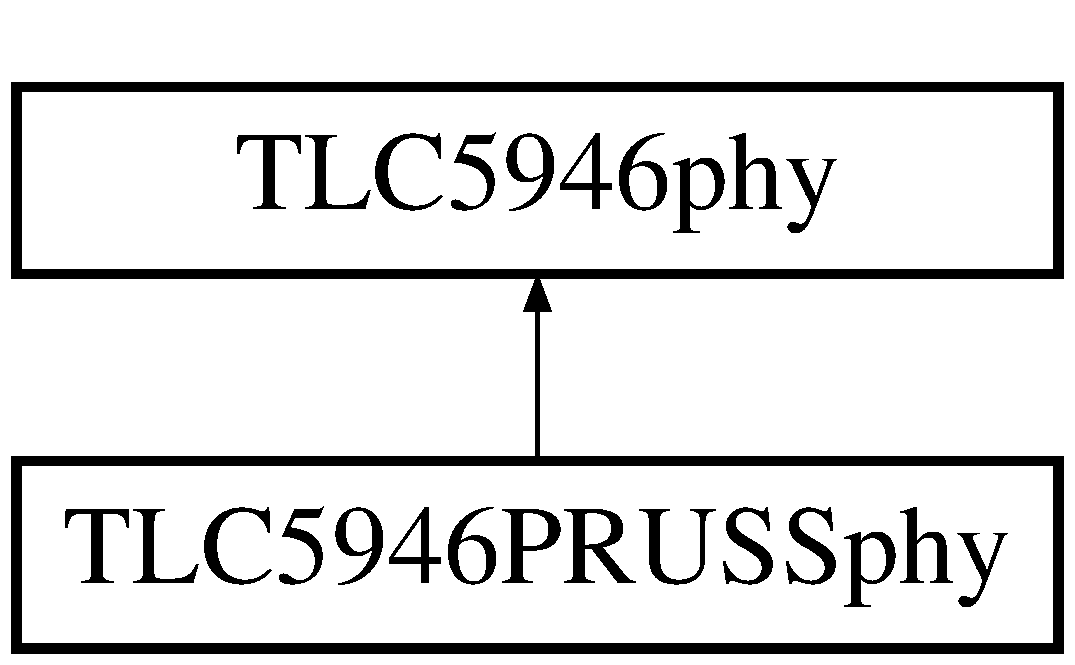
\includegraphics[height=2.000000cm]{class_t_l_c5946phy}
\end{center}
\end{figure}
\subsection*{Public Member Functions}
\begin{DoxyCompactItemize}
\item 
\hyperlink{class_t_l_c5946phy_acd5f2ca20ca8916c23625aca73306415}{T\-L\-C5946phy} (\hyperlink{class_s_p_i}{S\-P\-I} $\ast$\-\_\-spi, \hyperlink{class_g_p_i_opin}{G\-P\-I\-Opin} $\ast$\hyperlink{class_t_l_c5946phy_ad593ca4b96986ce8e40c833ed5ed3769}{ctrl})
\item 
virtual \hyperlink{class_t_l_c5946phy_a7ed74634384c99c3b305e0c33d9ec47b}{$\sim$\-T\-L\-C5946phy} ()
\item 
virtual void \hyperlink{class_t_l_c5946phy_a917d05cee794f633a6775b8c509efba0}{set\-Blank} (uint8\-\_\-t blank)
\item 
virtual void \hyperlink{class_t_l_c5946phy_a43974eb64479ebd593ea122e5f446ffa}{set\-Mode} (uint8\-\_\-t mode)
\item 
virtual void \hyperlink{class_t_l_c5946phy_a11b29859983d81add34d6fb0721613a2}{set\-Xhalf} (uint8\-\_\-t xhalf)
\item 
virtual uint8\-\_\-t \hyperlink{class_t_l_c5946phy_ac57ced207378247e87f025e3cb94d754}{get\-Xerr} ()
\item 
virtual int \hyperlink{class_t_l_c5946phy_a0604df91a14451f72504f39cd379eed1}{set\-Bits\-Per\-Word} (int bits)
\item 
virtual int \hyperlink{class_t_l_c5946phy_a7f12198f25476c730e6838cfcd94c388}{set\-L\-S\-B\-First} (bool lsb\-\_\-first)
\item 
virtual int \hyperlink{class_t_l_c5946phy_a142002ef92f3bb22579e63b9110e6a30}{xfer} (uint8\-\_\-t buf\-\_\-out\mbox{[}$\,$\mbox{]}, uint8\-\_\-t buf\-\_\-in\mbox{[}$\,$\mbox{]}, int len)
\end{DoxyCompactItemize}
\subsection*{Protected Attributes}
\begin{DoxyCompactItemize}
\item 
\hyperlink{class_s_p_i}{S\-P\-I} $\ast$ \hyperlink{class_t_l_c5946phy_aa1cd89ab21c1ce96acc6d2cc8af4136e}{spi}
\item 
\hyperlink{class_g_p_i_opin}{G\-P\-I\-Opin} $\ast$ \hyperlink{class_t_l_c5946phy_ad593ca4b96986ce8e40c833ed5ed3769}{ctrl}
\item 
bool \hyperlink{class_t_l_c5946phy_a6f0eea08d31a0209e5bc561b93a43067}{active}
\item 
int \hyperlink{class_t_l_c5946phy_a99fc1c99ddad63c7a7b15034ac9cffda}{blank\-\_\-pin\-\_\-pin}
\item 
int \hyperlink{class_t_l_c5946phy_a21c925ef7ce83c48daaebb56f994a720}{mode\-\_\-pin\-\_\-pin}
\item 
int \hyperlink{class_t_l_c5946phy_a072b879adb9d018b4a9905b53cb497f0}{xhalf\-\_\-pin\-\_\-pin}
\item 
int \hyperlink{class_t_l_c5946phy_a4c79de11b56731d25e7f0f0455b960f0}{xerr\-\_\-pin\-\_\-pin}
\end{DoxyCompactItemize}


\subsection{Detailed Description}
The class acts as a layer abstracting physical interface to T\-L\-C5946. Higher level class controlling behavior of the chain of the chips can call functions of the interface without needing to know how they interface with the actual hardware. This allows to implement high-\/level functionality without knowing how the hardware interface works. 

\subsection{Constructor \& Destructor Documentation}
\hypertarget{class_t_l_c5946phy_acd5f2ca20ca8916c23625aca73306415}{\index{T\-L\-C5946phy@{T\-L\-C5946phy}!T\-L\-C5946phy@{T\-L\-C5946phy}}
\index{T\-L\-C5946phy@{T\-L\-C5946phy}!TLC5946phy@{T\-L\-C5946phy}}
\subsubsection[{T\-L\-C5946phy}]{\setlength{\rightskip}{0pt plus 5cm}T\-L\-C5946phy\-::\-T\-L\-C5946phy (
\begin{DoxyParamCaption}
\item[{{\bf S\-P\-I} $\ast$}]{\-\_\-spi, }
\item[{{\bf G\-P\-I\-Opin} $\ast$}]{ctrl}
\end{DoxyParamCaption}
)}}\label{class_t_l_c5946phy_acd5f2ca20ca8916c23625aca73306415}
Constructor initializes T\-L\-C5946 physical interface using provided \hyperlink{class_s_p_i}{S\-P\-I} bus for data communication and G\-P\-I\-O lines as control signals. Constructor assumes that the clocking and blanking signals for the chip are generated externally and will not attempt to set them up. The \char`\"{}blank\char`\"{} line acts as \char`\"{}true\char`\"{} blank\-: setting the line active will blank all the outputs.

Control signals should be assigned the following names\-:
\begin{DoxyItemize}
\item mode
\item xhalf
\item xerr
\item blank
\end{DoxyItemize}

G\-S\-C\-L\-K line will not be used and does not need to be allocated.


\begin{DoxyParams}{Parameters}
{\em \-\_\-spi} & \\
\hline
{\em ctrl} & \\
\hline
\end{DoxyParams}
\hypertarget{class_t_l_c5946phy_a7ed74634384c99c3b305e0c33d9ec47b}{\index{T\-L\-C5946phy@{T\-L\-C5946phy}!$\sim$\-T\-L\-C5946phy@{$\sim$\-T\-L\-C5946phy}}
\index{$\sim$\-T\-L\-C5946phy@{$\sim$\-T\-L\-C5946phy}!TLC5946phy@{T\-L\-C5946phy}}
\subsubsection[{$\sim$\-T\-L\-C5946phy}]{\setlength{\rightskip}{0pt plus 5cm}T\-L\-C5946phy\-::$\sim$\-T\-L\-C5946phy (
\begin{DoxyParamCaption}
{}
\end{DoxyParamCaption}
)\hspace{0.3cm}{\ttfamily [virtual]}}}\label{class_t_l_c5946phy_a7ed74634384c99c3b305e0c33d9ec47b}


\subsection{Member Function Documentation}
\hypertarget{class_t_l_c5946phy_ac57ced207378247e87f025e3cb94d754}{\index{T\-L\-C5946phy@{T\-L\-C5946phy}!get\-Xerr@{get\-Xerr}}
\index{get\-Xerr@{get\-Xerr}!TLC5946phy@{T\-L\-C5946phy}}
\subsubsection[{get\-Xerr}]{\setlength{\rightskip}{0pt plus 5cm}uint8\-\_\-t T\-L\-C5946phy\-::get\-Xerr (
\begin{DoxyParamCaption}
{}
\end{DoxyParamCaption}
)\hspace{0.3cm}{\ttfamily [virtual]}}}\label{class_t_l_c5946phy_ac57ced207378247e87f025e3cb94d754}
\hypertarget{class_t_l_c5946phy_a0604df91a14451f72504f39cd379eed1}{\index{T\-L\-C5946phy@{T\-L\-C5946phy}!set\-Bits\-Per\-Word@{set\-Bits\-Per\-Word}}
\index{set\-Bits\-Per\-Word@{set\-Bits\-Per\-Word}!TLC5946phy@{T\-L\-C5946phy}}
\subsubsection[{set\-Bits\-Per\-Word}]{\setlength{\rightskip}{0pt plus 5cm}int T\-L\-C5946phy\-::set\-Bits\-Per\-Word (
\begin{DoxyParamCaption}
\item[{int}]{bits}
\end{DoxyParamCaption}
)\hspace{0.3cm}{\ttfamily [virtual]}}}\label{class_t_l_c5946phy_a0604df91a14451f72504f39cd379eed1}
\hypertarget{class_t_l_c5946phy_a917d05cee794f633a6775b8c509efba0}{\index{T\-L\-C5946phy@{T\-L\-C5946phy}!set\-Blank@{set\-Blank}}
\index{set\-Blank@{set\-Blank}!TLC5946phy@{T\-L\-C5946phy}}
\subsubsection[{set\-Blank}]{\setlength{\rightskip}{0pt plus 5cm}void T\-L\-C5946phy\-::set\-Blank (
\begin{DoxyParamCaption}
\item[{uint8\-\_\-t}]{blank}
\end{DoxyParamCaption}
)\hspace{0.3cm}{\ttfamily [virtual]}}}\label{class_t_l_c5946phy_a917d05cee794f633a6775b8c509efba0}


Reimplemented in \hyperlink{class_t_l_c5946_p_r_u_s_sphy_a28d5f0a3fb62b085dd7795373b9b4b85}{T\-L\-C5946\-P\-R\-U\-S\-Sphy}.

\hypertarget{class_t_l_c5946phy_a7f12198f25476c730e6838cfcd94c388}{\index{T\-L\-C5946phy@{T\-L\-C5946phy}!set\-L\-S\-B\-First@{set\-L\-S\-B\-First}}
\index{set\-L\-S\-B\-First@{set\-L\-S\-B\-First}!TLC5946phy@{T\-L\-C5946phy}}
\subsubsection[{set\-L\-S\-B\-First}]{\setlength{\rightskip}{0pt plus 5cm}int T\-L\-C5946phy\-::set\-L\-S\-B\-First (
\begin{DoxyParamCaption}
\item[{bool}]{lsb\-\_\-first}
\end{DoxyParamCaption}
)\hspace{0.3cm}{\ttfamily [virtual]}}}\label{class_t_l_c5946phy_a7f12198f25476c730e6838cfcd94c388}
\hypertarget{class_t_l_c5946phy_a43974eb64479ebd593ea122e5f446ffa}{\index{T\-L\-C5946phy@{T\-L\-C5946phy}!set\-Mode@{set\-Mode}}
\index{set\-Mode@{set\-Mode}!TLC5946phy@{T\-L\-C5946phy}}
\subsubsection[{set\-Mode}]{\setlength{\rightskip}{0pt plus 5cm}void T\-L\-C5946phy\-::set\-Mode (
\begin{DoxyParamCaption}
\item[{uint8\-\_\-t}]{mode}
\end{DoxyParamCaption}
)\hspace{0.3cm}{\ttfamily [virtual]}}}\label{class_t_l_c5946phy_a43974eb64479ebd593ea122e5f446ffa}
\hypertarget{class_t_l_c5946phy_a11b29859983d81add34d6fb0721613a2}{\index{T\-L\-C5946phy@{T\-L\-C5946phy}!set\-Xhalf@{set\-Xhalf}}
\index{set\-Xhalf@{set\-Xhalf}!TLC5946phy@{T\-L\-C5946phy}}
\subsubsection[{set\-Xhalf}]{\setlength{\rightskip}{0pt plus 5cm}void T\-L\-C5946phy\-::set\-Xhalf (
\begin{DoxyParamCaption}
\item[{uint8\-\_\-t}]{xhalf}
\end{DoxyParamCaption}
)\hspace{0.3cm}{\ttfamily [virtual]}}}\label{class_t_l_c5946phy_a11b29859983d81add34d6fb0721613a2}
\hypertarget{class_t_l_c5946phy_a142002ef92f3bb22579e63b9110e6a30}{\index{T\-L\-C5946phy@{T\-L\-C5946phy}!xfer@{xfer}}
\index{xfer@{xfer}!TLC5946phy@{T\-L\-C5946phy}}
\subsubsection[{xfer}]{\setlength{\rightskip}{0pt plus 5cm}int T\-L\-C5946phy\-::xfer (
\begin{DoxyParamCaption}
\item[{uint8\-\_\-t}]{buf\-\_\-out\mbox{[}$\,$\mbox{]}, }
\item[{uint8\-\_\-t}]{buf\-\_\-in\mbox{[}$\,$\mbox{]}, }
\item[{int}]{len}
\end{DoxyParamCaption}
)\hspace{0.3cm}{\ttfamily [virtual]}}}\label{class_t_l_c5946phy_a142002ef92f3bb22579e63b9110e6a30}


\subsection{Member Data Documentation}
\hypertarget{class_t_l_c5946phy_a6f0eea08d31a0209e5bc561b93a43067}{\index{T\-L\-C5946phy@{T\-L\-C5946phy}!active@{active}}
\index{active@{active}!TLC5946phy@{T\-L\-C5946phy}}
\subsubsection[{active}]{\setlength{\rightskip}{0pt plus 5cm}bool T\-L\-C5946phy\-::active\hspace{0.3cm}{\ttfamily [protected]}}}\label{class_t_l_c5946phy_a6f0eea08d31a0209e5bc561b93a43067}
\hypertarget{class_t_l_c5946phy_a99fc1c99ddad63c7a7b15034ac9cffda}{\index{T\-L\-C5946phy@{T\-L\-C5946phy}!blank\-\_\-pin\-\_\-pin@{blank\-\_\-pin\-\_\-pin}}
\index{blank\-\_\-pin\-\_\-pin@{blank\-\_\-pin\-\_\-pin}!TLC5946phy@{T\-L\-C5946phy}}
\subsubsection[{blank\-\_\-pin\-\_\-pin}]{\setlength{\rightskip}{0pt plus 5cm}int T\-L\-C5946phy\-::blank\-\_\-pin\-\_\-pin\hspace{0.3cm}{\ttfamily [protected]}}}\label{class_t_l_c5946phy_a99fc1c99ddad63c7a7b15034ac9cffda}
\hypertarget{class_t_l_c5946phy_ad593ca4b96986ce8e40c833ed5ed3769}{\index{T\-L\-C5946phy@{T\-L\-C5946phy}!ctrl@{ctrl}}
\index{ctrl@{ctrl}!TLC5946phy@{T\-L\-C5946phy}}
\subsubsection[{ctrl}]{\setlength{\rightskip}{0pt plus 5cm}{\bf G\-P\-I\-Opin}$\ast$ T\-L\-C5946phy\-::ctrl\hspace{0.3cm}{\ttfamily [protected]}}}\label{class_t_l_c5946phy_ad593ca4b96986ce8e40c833ed5ed3769}
\hypertarget{class_t_l_c5946phy_a21c925ef7ce83c48daaebb56f994a720}{\index{T\-L\-C5946phy@{T\-L\-C5946phy}!mode\-\_\-pin\-\_\-pin@{mode\-\_\-pin\-\_\-pin}}
\index{mode\-\_\-pin\-\_\-pin@{mode\-\_\-pin\-\_\-pin}!TLC5946phy@{T\-L\-C5946phy}}
\subsubsection[{mode\-\_\-pin\-\_\-pin}]{\setlength{\rightskip}{0pt plus 5cm}int T\-L\-C5946phy\-::mode\-\_\-pin\-\_\-pin\hspace{0.3cm}{\ttfamily [protected]}}}\label{class_t_l_c5946phy_a21c925ef7ce83c48daaebb56f994a720}
\hypertarget{class_t_l_c5946phy_aa1cd89ab21c1ce96acc6d2cc8af4136e}{\index{T\-L\-C5946phy@{T\-L\-C5946phy}!spi@{spi}}
\index{spi@{spi}!TLC5946phy@{T\-L\-C5946phy}}
\subsubsection[{spi}]{\setlength{\rightskip}{0pt plus 5cm}{\bf S\-P\-I}$\ast$ T\-L\-C5946phy\-::spi\hspace{0.3cm}{\ttfamily [protected]}}}\label{class_t_l_c5946phy_aa1cd89ab21c1ce96acc6d2cc8af4136e}
\hypertarget{class_t_l_c5946phy_a4c79de11b56731d25e7f0f0455b960f0}{\index{T\-L\-C5946phy@{T\-L\-C5946phy}!xerr\-\_\-pin\-\_\-pin@{xerr\-\_\-pin\-\_\-pin}}
\index{xerr\-\_\-pin\-\_\-pin@{xerr\-\_\-pin\-\_\-pin}!TLC5946phy@{T\-L\-C5946phy}}
\subsubsection[{xerr\-\_\-pin\-\_\-pin}]{\setlength{\rightskip}{0pt plus 5cm}int T\-L\-C5946phy\-::xerr\-\_\-pin\-\_\-pin\hspace{0.3cm}{\ttfamily [protected]}}}\label{class_t_l_c5946phy_a4c79de11b56731d25e7f0f0455b960f0}
\hypertarget{class_t_l_c5946phy_a072b879adb9d018b4a9905b53cb497f0}{\index{T\-L\-C5946phy@{T\-L\-C5946phy}!xhalf\-\_\-pin\-\_\-pin@{xhalf\-\_\-pin\-\_\-pin}}
\index{xhalf\-\_\-pin\-\_\-pin@{xhalf\-\_\-pin\-\_\-pin}!TLC5946phy@{T\-L\-C5946phy}}
\subsubsection[{xhalf\-\_\-pin\-\_\-pin}]{\setlength{\rightskip}{0pt plus 5cm}int T\-L\-C5946phy\-::xhalf\-\_\-pin\-\_\-pin\hspace{0.3cm}{\ttfamily [protected]}}}\label{class_t_l_c5946phy_a072b879adb9d018b4a9905b53cb497f0}


The documentation for this class was generated from the following files\-:\begin{DoxyCompactItemize}
\item 
include/device/\hyperlink{_t_l_c5946phy_8h}{T\-L\-C5946phy.\-h}\item 
src/\hyperlink{_t_l_c5946phy_8cpp}{T\-L\-C5946phy.\-cpp}\end{DoxyCompactItemize}

\hypertarget{class_t_l_c5946_p_r_u_s_sphy}{\section{T\-L\-C5946\-P\-R\-U\-S\-Sphy Class Reference}
\label{class_t_l_c5946_p_r_u_s_sphy}\index{T\-L\-C5946\-P\-R\-U\-S\-Sphy@{T\-L\-C5946\-P\-R\-U\-S\-Sphy}}
}


{\ttfamily \#include $<$T\-L\-C5946\-P\-R\-U\-S\-Sphy.\-h$>$}

Inheritance diagram for T\-L\-C5946\-P\-R\-U\-S\-Sphy\-:\begin{figure}[H]
\begin{center}
\leavevmode
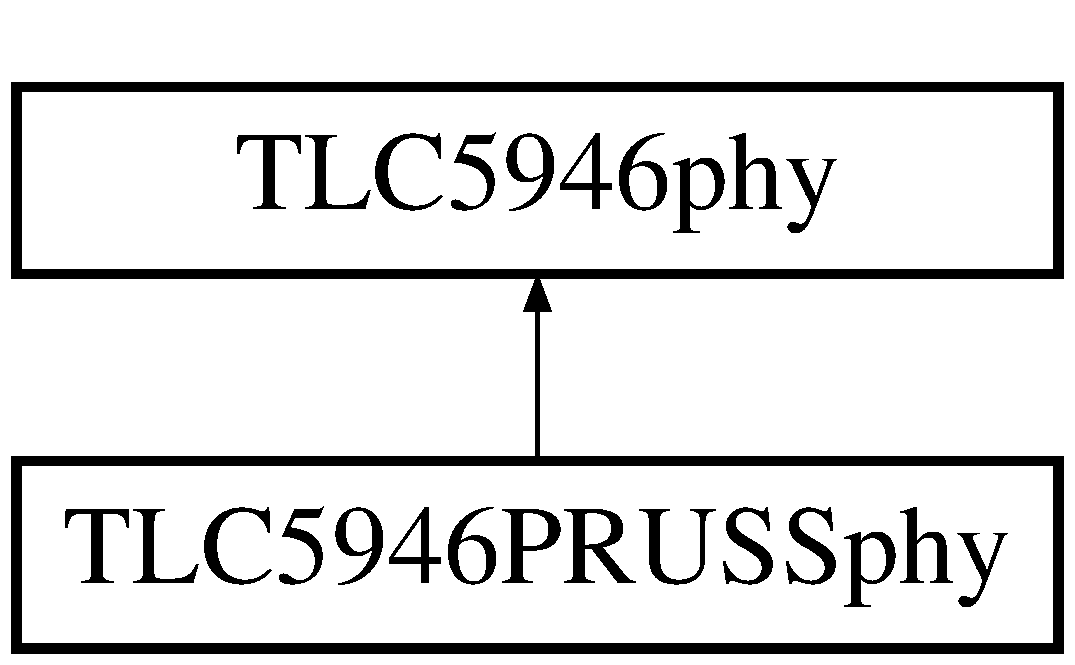
\includegraphics[height=2.000000cm]{class_t_l_c5946_p_r_u_s_sphy}
\end{center}
\end{figure}
\subsection*{Public Member Functions}
\begin{DoxyCompactItemize}
\item 
\hyperlink{class_t_l_c5946_p_r_u_s_sphy_a654892071d1aee78428b4c142151574d}{T\-L\-C5946\-P\-R\-U\-S\-Sphy} (\hyperlink{class_s_p_i}{S\-P\-I} $\ast$\-\_\-spi, \hyperlink{class_g_p_i_opin}{G\-P\-I\-Opin} $\ast$\hyperlink{class_t_l_c5946phy_ad593ca4b96986ce8e40c833ed5ed3769}{ctrl}, char $\ast$pru\-Bin\-File)
\item 
virtual \hyperlink{class_t_l_c5946_p_r_u_s_sphy_afe139acf9d6f593597a900e4311dab51}{$\sim$\-T\-L\-C5946\-P\-R\-U\-S\-Sphy} ()
\item 
virtual void \hyperlink{class_t_l_c5946_p_r_u_s_sphy_a28d5f0a3fb62b085dd7795373b9b4b85}{set\-Blank} (uint8\-\_\-t blank)
\end{DoxyCompactItemize}
\subsection*{Additional Inherited Members}


\subsection{Detailed Description}
The class acts as a layer abstracting physical interface to T\-L\-C5946. Higher level class controlling behavior of the chain of the chips can call functions of the interface without needing to know how they interface with the actual hardware. This allows to implement high-\/level functionality without knowing how the hardware interface works. 

\subsection{Constructor \& Destructor Documentation}
\hypertarget{class_t_l_c5946_p_r_u_s_sphy_a654892071d1aee78428b4c142151574d}{\index{T\-L\-C5946\-P\-R\-U\-S\-Sphy@{T\-L\-C5946\-P\-R\-U\-S\-Sphy}!T\-L\-C5946\-P\-R\-U\-S\-Sphy@{T\-L\-C5946\-P\-R\-U\-S\-Sphy}}
\index{T\-L\-C5946\-P\-R\-U\-S\-Sphy@{T\-L\-C5946\-P\-R\-U\-S\-Sphy}!TLC5946PRUSSphy@{T\-L\-C5946\-P\-R\-U\-S\-Sphy}}
\subsubsection[{T\-L\-C5946\-P\-R\-U\-S\-Sphy}]{\setlength{\rightskip}{0pt plus 5cm}T\-L\-C5946\-P\-R\-U\-S\-Sphy\-::\-T\-L\-C5946\-P\-R\-U\-S\-Sphy (
\begin{DoxyParamCaption}
\item[{{\bf S\-P\-I} $\ast$}]{\-\_\-spi, }
\item[{{\bf G\-P\-I\-Opin} $\ast$}]{ctrl, }
\item[{char $\ast$}]{pru\-Bin\-File}
\end{DoxyParamCaption}
)}}\label{class_t_l_c5946_p_r_u_s_sphy_a654892071d1aee78428b4c142151574d}
Constructor initializes T\-L\-C5946 physical interface using provided \hyperlink{class_s_p_i}{S\-P\-I} bus for data communication and G\-P\-I\-O lines as control signals. Constructor initializes P\-R\-U0 unit with microcode read from the file whose name is provided as the last parameter. The microcode should generate clocking and blanking sequences required by T\-L\-C5946 chip. If the microcode can not be read from the file or P\-R\-U\-S\-S can not be initialized, the module will not be activated.

Control signals should be assigned the following names\-:
\begin{DoxyItemize}
\item mode
\item xhalf
\item xerr
\item blank
\item gsclk
\end{DoxyItemize}

This function is Beaglebone-\/specific. 
\begin{DoxyParams}{Parameters}
{\em \-\_\-spi} & \\
\hline
{\em ctrl} & \\
\hline
{\em pru\-Bin\-File} & \\
\hline
\end{DoxyParams}
\hypertarget{class_t_l_c5946_p_r_u_s_sphy_afe139acf9d6f593597a900e4311dab51}{\index{T\-L\-C5946\-P\-R\-U\-S\-Sphy@{T\-L\-C5946\-P\-R\-U\-S\-Sphy}!$\sim$\-T\-L\-C5946\-P\-R\-U\-S\-Sphy@{$\sim$\-T\-L\-C5946\-P\-R\-U\-S\-Sphy}}
\index{$\sim$\-T\-L\-C5946\-P\-R\-U\-S\-Sphy@{$\sim$\-T\-L\-C5946\-P\-R\-U\-S\-Sphy}!TLC5946PRUSSphy@{T\-L\-C5946\-P\-R\-U\-S\-Sphy}}
\subsubsection[{$\sim$\-T\-L\-C5946\-P\-R\-U\-S\-Sphy}]{\setlength{\rightskip}{0pt plus 5cm}T\-L\-C5946\-P\-R\-U\-S\-Sphy\-::$\sim$\-T\-L\-C5946\-P\-R\-U\-S\-Sphy (
\begin{DoxyParamCaption}
{}
\end{DoxyParamCaption}
)\hspace{0.3cm}{\ttfamily [virtual]}}}\label{class_t_l_c5946_p_r_u_s_sphy_afe139acf9d6f593597a900e4311dab51}


\subsection{Member Function Documentation}
\hypertarget{class_t_l_c5946_p_r_u_s_sphy_a28d5f0a3fb62b085dd7795373b9b4b85}{\index{T\-L\-C5946\-P\-R\-U\-S\-Sphy@{T\-L\-C5946\-P\-R\-U\-S\-Sphy}!set\-Blank@{set\-Blank}}
\index{set\-Blank@{set\-Blank}!TLC5946PRUSSphy@{T\-L\-C5946\-P\-R\-U\-S\-Sphy}}
\subsubsection[{set\-Blank}]{\setlength{\rightskip}{0pt plus 5cm}void T\-L\-C5946\-P\-R\-U\-S\-Sphy\-::set\-Blank (
\begin{DoxyParamCaption}
\item[{uint8\-\_\-t}]{blank}
\end{DoxyParamCaption}
)\hspace{0.3cm}{\ttfamily [virtual]}}}\label{class_t_l_c5946_p_r_u_s_sphy_a28d5f0a3fb62b085dd7795373b9b4b85}


Reimplemented from \hyperlink{class_t_l_c5946phy_a917d05cee794f633a6775b8c509efba0}{T\-L\-C5946phy}.



The documentation for this class was generated from the following files\-:\begin{DoxyCompactItemize}
\item 
include/device/\hyperlink{_t_l_c5946_p_r_u_s_sphy_8h}{T\-L\-C5946\-P\-R\-U\-S\-Sphy.\-h}\item 
src/\hyperlink{_t_l_c5946_p_r_u_s_sphy_8cpp}{T\-L\-C5946\-P\-R\-U\-S\-Sphy.\-cpp}\end{DoxyCompactItemize}

\chapter{File Documentation}
\hypertarget{_beaglebone_s_p_i_8cpp}{\section{examples/\-Beaglebone\-S\-P\-I.cpp File Reference}
\label{_beaglebone_s_p_i_8cpp}\index{examples/\-Beaglebone\-S\-P\-I.\-cpp@{examples/\-Beaglebone\-S\-P\-I.\-cpp}}
}
{\ttfamily \#include $<$iostream$>$}\\*
{\ttfamily \#include $<$stdio.\-h$>$}\\*
{\ttfamily \#include $<$stdlib.\-h$>$}\\*
{\ttfamily \#include $<$math.\-h$>$}\\*
{\ttfamily \#include $<$pruss/prussdrv.\-h$>$}\\*
{\ttfamily \#include $<$pruss/pruss\-\_\-intc\-\_\-mapping.\-h$>$}\\*
{\ttfamily \#include $<$errno.\-h$>$}\\*
{\ttfamily \#include \char`\"{}S\-P\-I.\-h\char`\"{}}\\*
{\ttfamily \#include \char`\"{}G\-P\-I\-Ooo.\-h\char`\"{}}\\*
{\ttfamily \#include \char`\"{}G\-P\-I\-Opin.\-h\char`\"{}}\\*
{\ttfamily \#include \char`\"{}device/\-H\-D44780gpio\-Phy.\-h\char`\"{}}\\*
{\ttfamily \#include \char`\"{}device/\-H\-D44780.\-h\char`\"{}}\\*
{\ttfamily \#include \char`\"{}device/\-T\-L\-C5946phy.\-h\char`\"{}}\\*
{\ttfamily \#include \char`\"{}device/\-T\-L\-C5946chain.\-h\char`\"{}}\\*
{\ttfamily \#include \char`\"{}Test\-T\-L\-C5946.\-h\char`\"{}}\\*
{\ttfamily \#include \char`\"{}Test\-L\-C\-D.\-h\char`\"{}}\\*
{\ttfamily \#include \char`\"{}Test\-G\-P\-I\-O\-Leds.\-h\char`\"{}}\\*
{\ttfamily \#include \char`\"{}debug.\-h\char`\"{}}\\*
\subsection*{Macros}
\begin{DoxyCompactItemize}
\item 
\#define \hyperlink{_beaglebone_s_p_i_8cpp_a9bb61942a4e9c9cab56634ba82d06be9}{S\-E\-Q\-\_\-\-L\-E\-N}~10
\end{DoxyCompactItemize}
\subsection*{Functions}
\begin{DoxyCompactItemize}
\item 
int \hyperlink{_beaglebone_s_p_i_8cpp_a5f2aa15f0f163d1b32ecb4729c0ec8e7}{test\-S\-P\-I} (\hyperlink{class_s_p_i}{S\-P\-I} \&spi)
\item 
\hyperlink{class_s_p_i}{S\-P\-I} $\ast$ \hyperlink{_beaglebone_s_p_i_8cpp_ae764ad6d6eb2aecacdf8c31f41c2a276}{setup\-S\-P\-I} ()
\item 
int \hyperlink{_beaglebone_s_p_i_8cpp_ae66f6b31b5ad750f1fe042a706a4e3d4}{main} ()
\end{DoxyCompactItemize}


\subsection{Macro Definition Documentation}
\hypertarget{_beaglebone_s_p_i_8cpp_a9bb61942a4e9c9cab56634ba82d06be9}{\index{Beaglebone\-S\-P\-I.\-cpp@{Beaglebone\-S\-P\-I.\-cpp}!S\-E\-Q\-\_\-\-L\-E\-N@{S\-E\-Q\-\_\-\-L\-E\-N}}
\index{S\-E\-Q\-\_\-\-L\-E\-N@{S\-E\-Q\-\_\-\-L\-E\-N}!BeagleboneSPI.cpp@{Beaglebone\-S\-P\-I.\-cpp}}
\subsubsection[{S\-E\-Q\-\_\-\-L\-E\-N}]{\setlength{\rightskip}{0pt plus 5cm}\#define S\-E\-Q\-\_\-\-L\-E\-N~10}}\label{_beaglebone_s_p_i_8cpp_a9bb61942a4e9c9cab56634ba82d06be9}


\subsection{Function Documentation}
\hypertarget{_beaglebone_s_p_i_8cpp_ae66f6b31b5ad750f1fe042a706a4e3d4}{\index{Beaglebone\-S\-P\-I.\-cpp@{Beaglebone\-S\-P\-I.\-cpp}!main@{main}}
\index{main@{main}!BeagleboneSPI.cpp@{Beaglebone\-S\-P\-I.\-cpp}}
\subsubsection[{main}]{\setlength{\rightskip}{0pt plus 5cm}int main (
\begin{DoxyParamCaption}
{}
\end{DoxyParamCaption}
)}}\label{_beaglebone_s_p_i_8cpp_ae66f6b31b5ad750f1fe042a706a4e3d4}
\hypertarget{_beaglebone_s_p_i_8cpp_ae764ad6d6eb2aecacdf8c31f41c2a276}{\index{Beaglebone\-S\-P\-I.\-cpp@{Beaglebone\-S\-P\-I.\-cpp}!setup\-S\-P\-I@{setup\-S\-P\-I}}
\index{setup\-S\-P\-I@{setup\-S\-P\-I}!BeagleboneSPI.cpp@{Beaglebone\-S\-P\-I.\-cpp}}
\subsubsection[{setup\-S\-P\-I}]{\setlength{\rightskip}{0pt plus 5cm}{\bf S\-P\-I}$\ast$ setup\-S\-P\-I (
\begin{DoxyParamCaption}
{}
\end{DoxyParamCaption}
)}}\label{_beaglebone_s_p_i_8cpp_ae764ad6d6eb2aecacdf8c31f41c2a276}
\hypertarget{_beaglebone_s_p_i_8cpp_a5f2aa15f0f163d1b32ecb4729c0ec8e7}{\index{Beaglebone\-S\-P\-I.\-cpp@{Beaglebone\-S\-P\-I.\-cpp}!test\-S\-P\-I@{test\-S\-P\-I}}
\index{test\-S\-P\-I@{test\-S\-P\-I}!BeagleboneSPI.cpp@{Beaglebone\-S\-P\-I.\-cpp}}
\subsubsection[{test\-S\-P\-I}]{\setlength{\rightskip}{0pt plus 5cm}int test\-S\-P\-I (
\begin{DoxyParamCaption}
\item[{{\bf S\-P\-I} \&}]{spi}
\end{DoxyParamCaption}
)}}\label{_beaglebone_s_p_i_8cpp_a5f2aa15f0f163d1b32ecb4729c0ec8e7}

\hypertarget{gpio__buttons_8cpp}{\section{examples/gpio\-\_\-buttons.cpp File Reference}
\label{gpio__buttons_8cpp}\index{examples/gpio\-\_\-buttons.\-cpp@{examples/gpio\-\_\-buttons.\-cpp}}
}
{\ttfamily \#include $<$stdio.\-h$>$}\\*
{\ttfamily \#include $<$stdlib.\-h$>$}\\*
{\ttfamily \#include $<$errno.\-h$>$}\\*
{\ttfamily \#include \char`\"{}Test\-G\-P\-I\-O\-Buttons.\-h\char`\"{}}\\*
\subsection*{Functions}
\begin{DoxyCompactItemize}
\item 
int \hyperlink{gpio__buttons_8cpp_ae66f6b31b5ad750f1fe042a706a4e3d4}{main} ()
\end{DoxyCompactItemize}


\subsection{Function Documentation}
\hypertarget{gpio__buttons_8cpp_ae66f6b31b5ad750f1fe042a706a4e3d4}{\index{gpio\-\_\-buttons.\-cpp@{gpio\-\_\-buttons.\-cpp}!main@{main}}
\index{main@{main}!gpio_buttons.cpp@{gpio\-\_\-buttons.\-cpp}}
\subsubsection[{main}]{\setlength{\rightskip}{0pt plus 5cm}int main (
\begin{DoxyParamCaption}
{}
\end{DoxyParamCaption}
)}}\label{gpio__buttons_8cpp_ae66f6b31b5ad750f1fe042a706a4e3d4}

\hypertarget{gpio__lcd_8cpp}{\section{examples/gpio\-\_\-lcd.cpp File Reference}
\label{gpio__lcd_8cpp}\index{examples/gpio\-\_\-lcd.\-cpp@{examples/gpio\-\_\-lcd.\-cpp}}
}
{\ttfamily \#include $<$stdio.\-h$>$}\\*
{\ttfamily \#include $<$stdlib.\-h$>$}\\*
{\ttfamily \#include \char`\"{}G\-P\-I\-Ooo.\-h\char`\"{}}\\*
{\ttfamily \#include \char`\"{}G\-P\-I\-Opin.\-h\char`\"{}}\\*
{\ttfamily \#include \char`\"{}device/\-H\-D44780gpio\-Phy.\-h\char`\"{}}\\*
{\ttfamily \#include \char`\"{}device/\-H\-D44780.\-h\char`\"{}}\\*
{\ttfamily \#include \char`\"{}Test\-L\-C\-D.\-h\char`\"{}}\\*
{\ttfamily \#include \char`\"{}debug.\-h\char`\"{}}\\*
\subsection*{Functions}
\begin{DoxyCompactItemize}
\item 
int \hyperlink{gpio__lcd_8cpp_ae66f6b31b5ad750f1fe042a706a4e3d4}{main} ()
\end{DoxyCompactItemize}


\subsection{Function Documentation}
\hypertarget{gpio__lcd_8cpp_ae66f6b31b5ad750f1fe042a706a4e3d4}{\index{gpio\-\_\-lcd.\-cpp@{gpio\-\_\-lcd.\-cpp}!main@{main}}
\index{main@{main}!gpio_lcd.cpp@{gpio\-\_\-lcd.\-cpp}}
\subsubsection[{main}]{\setlength{\rightskip}{0pt plus 5cm}int main (
\begin{DoxyParamCaption}
{}
\end{DoxyParamCaption}
)}}\label{gpio__lcd_8cpp_ae66f6b31b5ad750f1fe042a706a4e3d4}

\hypertarget{gpio__leds_8cpp}{\section{examples/gpio\-\_\-leds.cpp File Reference}
\label{gpio__leds_8cpp}\index{examples/gpio\-\_\-leds.\-cpp@{examples/gpio\-\_\-leds.\-cpp}}
}
{\ttfamily \#include $<$stdio.\-h$>$}\\*
{\ttfamily \#include $<$stdlib.\-h$>$}\\*
{\ttfamily \#include $<$errno.\-h$>$}\\*
{\ttfamily \#include \char`\"{}Test\-G\-P\-I\-O\-Leds.\-h\char`\"{}}\\*
{\ttfamily \#include \char`\"{}debug.\-h\char`\"{}}\\*
\subsection*{Functions}
\begin{DoxyCompactItemize}
\item 
int \hyperlink{gpio__leds_8cpp_ae66f6b31b5ad750f1fe042a706a4e3d4}{main} ()
\end{DoxyCompactItemize}


\subsection{Function Documentation}
\hypertarget{gpio__leds_8cpp_ae66f6b31b5ad750f1fe042a706a4e3d4}{\index{gpio\-\_\-leds.\-cpp@{gpio\-\_\-leds.\-cpp}!main@{main}}
\index{main@{main}!gpio_leds.cpp@{gpio\-\_\-leds.\-cpp}}
\subsubsection[{main}]{\setlength{\rightskip}{0pt plus 5cm}int main (
\begin{DoxyParamCaption}
{}
\end{DoxyParamCaption}
)}}\label{gpio__leds_8cpp_ae66f6b31b5ad750f1fe042a706a4e3d4}

\hypertarget{pru__loader_8c}{\section{examples/pru\-\_\-loader.c File Reference}
\label{pru__loader_8c}\index{examples/pru\-\_\-loader.\-c@{examples/pru\-\_\-loader.\-c}}
}
{\ttfamily \#include $<$errno.\-h$>$}\\*
{\ttfamily \#include $<$stdio.\-h$>$}\\*
{\ttfamily \#include $<$stdint.\-h$>$}\\*
{\ttfamily \#include $<$stdlib.\-h$>$}\\*
{\ttfamily \#include $<$string.\-h$>$}\\*
{\ttfamily \#include $<$signal.\-h$>$}\\*
{\ttfamily \#include $<$unistd.\-h$>$}\\*
{\ttfamily \#include $<$pruss/prussdrv.\-h$>$}\\*
{\ttfamily \#include $<$pruss/pruss\-\_\-intc\-\_\-mapping.\-h$>$}\\*
{\ttfamily \#include $<$sys/fcntl.\-h$>$}\\*
{\ttfamily \#include $<$sys/stat.\-h$>$}\\*
{\ttfamily \#include $<$time.\-h$>$}\\*
\subsection*{Classes}
\begin{DoxyCompactItemize}
\item 
struct \hyperlink{structpru__data}{pru\-\_\-data}
\end{DoxyCompactItemize}
\subsection*{Functions}
\begin{DoxyCompactItemize}
\item 
int \hyperlink{pru__loader_8c_a3c04138a5bfe5d72780bb7e82a18e627}{main} (int argc, char $\ast$$\ast$argv)
\end{DoxyCompactItemize}


\subsection{Function Documentation}
\hypertarget{pru__loader_8c_a3c04138a5bfe5d72780bb7e82a18e627}{\index{pru\-\_\-loader.\-c@{pru\-\_\-loader.\-c}!main@{main}}
\index{main@{main}!pru_loader.c@{pru\-\_\-loader.\-c}}
\subsubsection[{main}]{\setlength{\rightskip}{0pt plus 5cm}int main (
\begin{DoxyParamCaption}
\item[{int}]{argc, }
\item[{char $\ast$$\ast$}]{argv}
\end{DoxyParamCaption}
)}}\label{pru__loader_8c_a3c04138a5bfe5d72780bb7e82a18e627}

\hypertarget{_test_g_p_i_o_buttons_8cpp}{\section{examples/\-Test\-G\-P\-I\-O\-Buttons.cpp File Reference}
\label{_test_g_p_i_o_buttons_8cpp}\index{examples/\-Test\-G\-P\-I\-O\-Buttons.\-cpp@{examples/\-Test\-G\-P\-I\-O\-Buttons.\-cpp}}
}
{\ttfamily \#include \char`\"{}Test\-G\-P\-I\-O\-Buttons.\-h\char`\"{}}\\*
{\ttfamily \#include \char`\"{}stdio.\-h\char`\"{}}\\*
{\ttfamily \#include \char`\"{}unistd.\-h\char`\"{}}\\*

\hypertarget{_test_g_p_i_o_buttons_8h}{\section{examples/\-Test\-G\-P\-I\-O\-Buttons.h File Reference}
\label{_test_g_p_i_o_buttons_8h}\index{examples/\-Test\-G\-P\-I\-O\-Buttons.\-h@{examples/\-Test\-G\-P\-I\-O\-Buttons.\-h}}
}
{\ttfamily \#include \char`\"{}G\-P\-I\-Ooo.\-h\char`\"{}}\\*
{\ttfamily \#include \char`\"{}G\-P\-I\-Opin.\-h\char`\"{}}\\*
\subsection*{Classes}
\begin{DoxyCompactItemize}
\item 
class \hyperlink{class_test_g_p_i_o_buttons}{Test\-G\-P\-I\-O\-Buttons}
\end{DoxyCompactItemize}

\hypertarget{_test_g_p_i_o_leds_8cpp}{\section{examples/\-Test\-G\-P\-I\-O\-Leds.cpp File Reference}
\label{_test_g_p_i_o_leds_8cpp}\index{examples/\-Test\-G\-P\-I\-O\-Leds.\-cpp@{examples/\-Test\-G\-P\-I\-O\-Leds.\-cpp}}
}
{\ttfamily \#include \char`\"{}Test\-G\-P\-I\-O\-Leds.\-h\char`\"{}}\\*
{\ttfamily \#include $<$unistd.\-h$>$}\\*

\hypertarget{_test_g_p_i_o_leds_8h}{\section{examples/\-Test\-G\-P\-I\-O\-Leds.h File Reference}
\label{_test_g_p_i_o_leds_8h}\index{examples/\-Test\-G\-P\-I\-O\-Leds.\-h@{examples/\-Test\-G\-P\-I\-O\-Leds.\-h}}
}
{\ttfamily \#include \char`\"{}G\-P\-I\-Ooo.\-h\char`\"{}}\\*
{\ttfamily \#include \char`\"{}G\-P\-I\-Opin.\-h\char`\"{}}\\*
\subsection*{Classes}
\begin{DoxyCompactItemize}
\item 
class \hyperlink{class_test_g_p_i_o_leds}{Test\-G\-P\-I\-O\-Leds}
\end{DoxyCompactItemize}

\hypertarget{_test_l_c_d_8cpp}{\section{examples/\-Test\-L\-C\-D.cpp File Reference}
\label{_test_l_c_d_8cpp}\index{examples/\-Test\-L\-C\-D.\-cpp@{examples/\-Test\-L\-C\-D.\-cpp}}
}
{\ttfamily \#include $<$stdio.\-h$>$}\\*
{\ttfamily \#include \char`\"{}Test\-L\-C\-D.\-h\char`\"{}}\\*
{\ttfamily \#include \char`\"{}debug.\-h\char`\"{}}\\*

\hypertarget{_test_l_c_d_8h}{\section{examples/\-Test\-L\-C\-D.h File Reference}
\label{_test_l_c_d_8h}\index{examples/\-Test\-L\-C\-D.\-h@{examples/\-Test\-L\-C\-D.\-h}}
}
{\ttfamily \#include \char`\"{}G\-P\-I\-Ooo.\-h\char`\"{}}\\*
{\ttfamily \#include \char`\"{}G\-P\-I\-Opin.\-h\char`\"{}}\\*
{\ttfamily \#include \char`\"{}device/\-H\-D44780gpio\-Phy.\-h\char`\"{}}\\*
{\ttfamily \#include \char`\"{}device/\-H\-D44780.\-h\char`\"{}}\\*
\subsection*{Classes}
\begin{DoxyCompactItemize}
\item 
class \hyperlink{class_test_l_c_d}{Test\-L\-C\-D}
\end{DoxyCompactItemize}

\hypertarget{_test_t_l_c5946_8cpp}{\section{examples/\-Test\-T\-L\-C5946.cpp File Reference}
\label{_test_t_l_c5946_8cpp}\index{examples/\-Test\-T\-L\-C5946.\-cpp@{examples/\-Test\-T\-L\-C5946.\-cpp}}
}
{\ttfamily \#include \char`\"{}Test\-T\-L\-C5946.\-h\char`\"{}}\\*
{\ttfamily \#include $<$math.\-h$>$}\\*
{\ttfamily \#include $<$stdio.\-h$>$}\\*
{\ttfamily \#include $<$stdlib.\-h$>$}\\*
{\ttfamily \#include $<$unistd.\-h$>$}\\*

\hypertarget{_test_t_l_c5946_8h}{\section{examples/\-Test\-T\-L\-C5946.h File Reference}
\label{_test_t_l_c5946_8h}\index{examples/\-Test\-T\-L\-C5946.\-h@{examples/\-Test\-T\-L\-C5946.\-h}}
}
{\ttfamily \#include \char`\"{}G\-P\-I\-Ooo.\-h\char`\"{}}\\*
{\ttfamily \#include \char`\"{}G\-P\-I\-Opin.\-h\char`\"{}}\\*
{\ttfamily \#include \char`\"{}device/\-T\-L\-C5946\-P\-R\-U\-S\-Sphy.\-h\char`\"{}}\\*
{\ttfamily \#include \char`\"{}device/\-T\-L\-C5946chain.\-h\char`\"{}}\\*
\subsection*{Classes}
\begin{DoxyCompactItemize}
\item 
class \hyperlink{class_test_t_l_c5946}{Test\-T\-L\-C5946}
\end{DoxyCompactItemize}

\hypertarget{tlc5946_8cpp}{\section{examples/tlc5946.cpp File Reference}
\label{tlc5946_8cpp}\index{examples/tlc5946.\-cpp@{examples/tlc5946.\-cpp}}
}
{\ttfamily \#include $<$stdio.\-h$>$}\\*
{\ttfamily \#include $<$stdlib.\-h$>$}\\*
{\ttfamily \#include $<$errno.\-h$>$}\\*
{\ttfamily \#include \char`\"{}S\-P\-I.\-h\char`\"{}}\\*
{\ttfamily \#include \char`\"{}G\-P\-I\-Ooo.\-h\char`\"{}}\\*
{\ttfamily \#include \char`\"{}G\-P\-I\-Opin.\-h\char`\"{}}\\*
{\ttfamily \#include \char`\"{}Test\-T\-L\-C5946.\-h\char`\"{}}\\*
{\ttfamily \#include \char`\"{}debug.\-h\char`\"{}}\\*
\subsection*{Functions}
\begin{DoxyCompactItemize}
\item 
\hyperlink{class_s_p_i}{S\-P\-I} $\ast$ \hyperlink{tlc5946_8cpp_ae764ad6d6eb2aecacdf8c31f41c2a276}{setup\-S\-P\-I} ()
\item 
int \hyperlink{tlc5946_8cpp_ae66f6b31b5ad750f1fe042a706a4e3d4}{main} ()
\end{DoxyCompactItemize}


\subsection{Function Documentation}
\hypertarget{tlc5946_8cpp_ae66f6b31b5ad750f1fe042a706a4e3d4}{\index{tlc5946.\-cpp@{tlc5946.\-cpp}!main@{main}}
\index{main@{main}!tlc5946.cpp@{tlc5946.\-cpp}}
\subsubsection[{main}]{\setlength{\rightskip}{0pt plus 5cm}int main (
\begin{DoxyParamCaption}
{}
\end{DoxyParamCaption}
)}}\label{tlc5946_8cpp_ae66f6b31b5ad750f1fe042a706a4e3d4}
\hypertarget{tlc5946_8cpp_ae764ad6d6eb2aecacdf8c31f41c2a276}{\index{tlc5946.\-cpp@{tlc5946.\-cpp}!setup\-S\-P\-I@{setup\-S\-P\-I}}
\index{setup\-S\-P\-I@{setup\-S\-P\-I}!tlc5946.cpp@{tlc5946.\-cpp}}
\subsubsection[{setup\-S\-P\-I}]{\setlength{\rightskip}{0pt plus 5cm}{\bf S\-P\-I}$\ast$ setup\-S\-P\-I (
\begin{DoxyParamCaption}
{}
\end{DoxyParamCaption}
)}}\label{tlc5946_8cpp_ae764ad6d6eb2aecacdf8c31f41c2a276}

\hypertarget{_beagle_goo_8h}{\section{include/beaglebone/\-Beagle\-Goo.h File Reference}
\label{_beagle_goo_8h}\index{include/beaglebone/\-Beagle\-Goo.\-h@{include/beaglebone/\-Beagle\-Goo.\-h}}
}
{\ttfamily \#include \char`\"{}../\-G\-P\-I\-Ooo.\-h\char`\"{}}\\*
{\ttfamily \#include $<$stdint.\-h$>$}\\*
\subsection*{Classes}
\begin{DoxyCompactItemize}
\item 
class \hyperlink{struct_beagle_goo}{Beagle\-Goo}
\item 
struct \hyperlink{struct_beagle_goo_1_1_g_p_i_o_info}{Beagle\-Goo\-::\-G\-P\-I\-O\-Info}
\end{DoxyCompactItemize}

\hypertarget{_beagle_goo_p_8h}{\section{include/beaglebone/\-Beagle\-Goo\-P.h File Reference}
\label{_beagle_goo_p_8h}\index{include/beaglebone/\-Beagle\-Goo\-P.\-h@{include/beaglebone/\-Beagle\-Goo\-P.\-h}}
}
{\ttfamily \#include \char`\"{}G\-P\-I\-Opin.\-h\char`\"{}}\\*
{\ttfamily \#include \char`\"{}Beagle\-Goo.\-h\char`\"{}}\\*
{\ttfamily \#include $<$stdint.\-h$>$}\\*
\subsection*{Classes}
\begin{DoxyCompactItemize}
\item 
class \hyperlink{class_beagle_goo_p}{Beagle\-Goo\-P}
\end{DoxyCompactItemize}

\hypertarget{debug_8h}{\section{include/debug.h File Reference}
\label{debug_8h}\index{include/debug.\-h@{include/debug.\-h}}
}
\subsection*{Macros}
\begin{DoxyCompactItemize}
\item 
\#define \hyperlink{debug_8h_ac2d33ccaf63f5d5b66552b95426c0137}{D\-E\-B\-U\-G\-\_\-\-L\-E\-V\-E\-L}~-\/1
\item 
\#define \hyperlink{debug_8h_a5ed91c6fa16b273dcf5a09956f7fa539}{debug}(level, format,...)~\{if(level$<$=\hyperlink{debug_8h_ac2d33ccaf63f5d5b66552b95426c0137}{D\-E\-B\-U\-G\-\_\-\-L\-E\-V\-E\-L})\{printf( \char`\"{}\%s\-:\%i\-:\char`\"{}\#format\char`\"{}\textbackslash{}n\char`\"{},\-\_\-\-\_\-\-F\-I\-L\-E\-\_\-\-\_\-,\-\_\-\-\_\-\-L\-I\-N\-E\-\_\-\-\_\-,\#\#\-\_\-\-\_\-\-V\-A\-\_\-\-A\-R\-G\-S\-\_\-\-\_\-);\}\}
\end{DoxyCompactItemize}


\subsection{Macro Definition Documentation}
\hypertarget{debug_8h_a5ed91c6fa16b273dcf5a09956f7fa539}{\index{debug.\-h@{debug.\-h}!debug@{debug}}
\index{debug@{debug}!debug.h@{debug.\-h}}
\subsubsection[{debug}]{\setlength{\rightskip}{0pt plus 5cm}\#define debug(
\begin{DoxyParamCaption}
\item[{}]{level, }
\item[{}]{format, }
\item[{}]{...}
\end{DoxyParamCaption}
)~\{if(level$<$={\bf D\-E\-B\-U\-G\-\_\-\-L\-E\-V\-E\-L})\{printf( \char`\"{}\%s\-:\%i\-:\char`\"{}\#format\char`\"{}\textbackslash{}n\char`\"{},\-\_\-\-\_\-\-F\-I\-L\-E\-\_\-\-\_\-,\-\_\-\-\_\-\-L\-I\-N\-E\-\_\-\-\_\-,\#\#\-\_\-\-\_\-\-V\-A\-\_\-\-A\-R\-G\-S\-\_\-\-\_\-);\}\}}}\label{debug_8h_a5ed91c6fa16b273dcf5a09956f7fa539}
Debug macro Params\-: 
\begin{DoxyParams}{Parameters}
{\em level} & -\/ level of details of debug message. \\
\hline
{\em format} & -\/ Formatting string for the debug message \\
\hline
{\em ...} & -\/ \\
\hline
\end{DoxyParams}
\hypertarget{debug_8h_ac2d33ccaf63f5d5b66552b95426c0137}{\index{debug.\-h@{debug.\-h}!D\-E\-B\-U\-G\-\_\-\-L\-E\-V\-E\-L@{D\-E\-B\-U\-G\-\_\-\-L\-E\-V\-E\-L}}
\index{D\-E\-B\-U\-G\-\_\-\-L\-E\-V\-E\-L@{D\-E\-B\-U\-G\-\_\-\-L\-E\-V\-E\-L}!debug.h@{debug.\-h}}
\subsubsection[{D\-E\-B\-U\-G\-\_\-\-L\-E\-V\-E\-L}]{\setlength{\rightskip}{0pt plus 5cm}\#define D\-E\-B\-U\-G\-\_\-\-L\-E\-V\-E\-L~-\/1}}\label{debug_8h_ac2d33ccaf63f5d5b66552b95426c0137}

\hypertarget{_h_d44780_8h}{\section{include/device/\-H\-D44780.h File Reference}
\label{_h_d44780_8h}\index{include/device/\-H\-D44780.\-h@{include/device/\-H\-D44780.\-h}}
}
{\ttfamily \#include \char`\"{}H\-D44780phy.\-h\char`\"{}}\\*
\subsection*{Classes}
\begin{DoxyCompactItemize}
\item 
class \hyperlink{class_h_d44780}{H\-D44780}
\end{DoxyCompactItemize}

\hypertarget{_h_d44780gpio_phy_8h}{\section{include/device/\-H\-D44780gpio\-Phy.h File Reference}
\label{_h_d44780gpio_phy_8h}\index{include/device/\-H\-D44780gpio\-Phy.\-h@{include/device/\-H\-D44780gpio\-Phy.\-h}}
}
{\ttfamily \#include \char`\"{}G\-P\-I\-Opin.\-h\char`\"{}}\\*
{\ttfamily \#include \char`\"{}H\-D44780phy.\-h\char`\"{}}\\*
\subsection*{Classes}
\begin{DoxyCompactItemize}
\item 
class \hyperlink{class_h_d44780gpio_phy}{H\-D44780gpio\-Phy}
\end{DoxyCompactItemize}

\hypertarget{_h_d44780phy_8h}{\section{include/device/\-H\-D44780phy.h File Reference}
\label{_h_d44780phy_8h}\index{include/device/\-H\-D44780phy.\-h@{include/device/\-H\-D44780phy.\-h}}
}
{\ttfamily \#include $<$stdint.\-h$>$}\\*
\subsection*{Classes}
\begin{DoxyCompactItemize}
\item 
class \hyperlink{class_h_d44780phy}{H\-D44780phy}
\end{DoxyCompactItemize}

\hypertarget{_t_l_c5946chain_8h}{\section{include/device/\-T\-L\-C5946chain.h File Reference}
\label{_t_l_c5946chain_8h}\index{include/device/\-T\-L\-C5946chain.\-h@{include/device/\-T\-L\-C5946chain.\-h}}
}
{\ttfamily \#include \char`\"{}T\-L\-C5946phy.\-h\char`\"{}}\\*
\subsection*{Classes}
\begin{DoxyCompactItemize}
\item 
class \hyperlink{class_t_l_c5946chain}{T\-L\-C5946chain}
\end{DoxyCompactItemize}

\hypertarget{_t_l_c5946phy_8h}{\section{include/device/\-T\-L\-C5946phy.h File Reference}
\label{_t_l_c5946phy_8h}\index{include/device/\-T\-L\-C5946phy.\-h@{include/device/\-T\-L\-C5946phy.\-h}}
}
{\ttfamily \#include \char`\"{}S\-P\-I.\-h\char`\"{}}\\*
{\ttfamily \#include \char`\"{}G\-P\-I\-Opin.\-h\char`\"{}}\\*
\subsection*{Classes}
\begin{DoxyCompactItemize}
\item 
class \hyperlink{class_t_l_c5946phy}{T\-L\-C5946phy}
\end{DoxyCompactItemize}

\hypertarget{_t_l_c5946_p_r_u_s_sphy_8h}{\section{include/device/\-T\-L\-C5946\-P\-R\-U\-S\-Sphy.h File Reference}
\label{_t_l_c5946_p_r_u_s_sphy_8h}\index{include/device/\-T\-L\-C5946\-P\-R\-U\-S\-Sphy.\-h@{include/device/\-T\-L\-C5946\-P\-R\-U\-S\-Sphy.\-h}}
}
{\ttfamily \#include \char`\"{}S\-P\-I.\-h\char`\"{}}\\*
{\ttfamily \#include \char`\"{}G\-P\-I\-Opin.\-h\char`\"{}}\\*
{\ttfamily \#include \char`\"{}T\-L\-C5946phy.\-h\char`\"{}}\\*
\subsection*{Classes}
\begin{DoxyCompactItemize}
\item 
class \hyperlink{class_t_l_c5946_p_r_u_s_sphy}{T\-L\-C5946\-P\-R\-U\-S\-Sphy}
\end{DoxyCompactItemize}

\hypertarget{_g_p_i_ooo_8h}{\section{include/\-G\-P\-I\-Ooo.h File Reference}
\label{_g_p_i_ooo_8h}\index{include/\-G\-P\-I\-Ooo.\-h@{include/\-G\-P\-I\-Ooo.\-h}}
}
{\ttfamily \#include \char`\"{}G\-P\-I\-Opin.\-h\char`\"{}}\\*
\subsection*{Classes}
\begin{DoxyCompactItemize}
\item 
class \hyperlink{class_g_p_i_ooo}{G\-P\-I\-Ooo}
\begin{DoxyCompactList}\small\item\em Object-\/oriented implementation of G\-P\-I\-O Class defines interface for object-\/oriented handling of G\-P\-I\-O operations. Should be used as parent class for platform-\/specific implementations. \end{DoxyCompactList}\end{DoxyCompactItemize}

\hypertarget{_g_p_i_opin_8h}{\section{include/\-G\-P\-I\-Opin.h File Reference}
\label{_g_p_i_opin_8h}\index{include/\-G\-P\-I\-Opin.\-h@{include/\-G\-P\-I\-Opin.\-h}}
}
{\ttfamily \#include $<$stdlib.\-h$>$}\\*
{\ttfamily \#include $<$stdint.\-h$>$}\\*
\subsection*{Classes}
\begin{DoxyCompactItemize}
\item 
class \hyperlink{class_g_p_i_opin}{G\-P\-I\-Opin}
\end{DoxyCompactItemize}

\hypertarget{_s_p_i_8h}{\section{include/\-S\-P\-I.h File Reference}
\label{_s_p_i_8h}\index{include/\-S\-P\-I.\-h@{include/\-S\-P\-I.\-h}}
}
{\ttfamily \#include $<$stdint.\-h$>$}\\*
{\ttfamily \#include $<$linux/spi/spidev.\-h$>$}\\*
\subsection*{Classes}
\begin{DoxyCompactItemize}
\item 
class \hyperlink{class_s_p_i}{S\-P\-I}
\end{DoxyCompactItemize}

\hypertarget{_beagle_goo_8cpp}{\section{src/\-Beagle\-Goo.cpp File Reference}
\label{_beagle_goo_8cpp}\index{src/\-Beagle\-Goo.\-cpp@{src/\-Beagle\-Goo.\-cpp}}
}
{\ttfamily \#include \char`\"{}beaglebone/\-Beagle\-Goo.\-h\char`\"{}}\\*
{\ttfamily \#include \char`\"{}beaglebone/\-Beagle\-Goo\-P.\-h\char`\"{}}\\*
{\ttfamily \#include $<$stdlib.\-h$>$}\\*
{\ttfamily \#include $<$stdio.\-h$>$}\\*
{\ttfamily \#include $<$string.\-h$>$}\\*
{\ttfamily \#include $<$unistd.\-h$>$}\\*
{\ttfamily \#include $<$fcntl.\-h$>$}\\*
{\ttfamily \#include $<$sys/mman.\-h$>$}\\*
{\ttfamily \#include \char`\"{}debug.\-h\char`\"{}}\\*
\subsection*{Classes}
\begin{DoxyCompactItemize}
\item 
class \hyperlink{struct_beagle_goo}{Beagle\-Goo}
\end{DoxyCompactItemize}

\hypertarget{_beagle_goo_p_8cpp}{\section{src/\-Beagle\-Goo\-P.cpp File Reference}
\label{_beagle_goo_p_8cpp}\index{src/\-Beagle\-Goo\-P.\-cpp@{src/\-Beagle\-Goo\-P.\-cpp}}
}
{\ttfamily \#include \char`\"{}beaglebone/\-Beagle\-Goo\-P.\-h\char`\"{}}\\*
{\ttfamily \#include $<$string.\-h$>$}\\*
{\ttfamily \#include $<$stdio.\-h$>$}\\*
{\ttfamily \#include \char`\"{}debug.\-h\char`\"{}}\\*
\subsection*{Macros}
\begin{DoxyCompactItemize}
\item 
\#define \hyperlink{_beagle_goo_p_8cpp_af042aacdd1e062b2be5de959f98e6ad2}{D\-A\-T\-A\-\_\-\-O\-U\-T\-\_\-\-R\-E\-G}~0x13\-C
\item 
\#define \hyperlink{_beagle_goo_p_8cpp_ae4f312b1c9bbb129860a307d8dcf40b8}{D\-A\-T\-A\-\_\-\-I\-N\-\_\-\-R\-E\-G}~0x138
\item 
\#define \hyperlink{_beagle_goo_p_8cpp_a192aee11f30b27525c51ff6004a6b116}{G\-P\-I\-O\-\_\-\-O\-E\-\_\-\-R\-E\-G}~0x134
\item 
\#define \hyperlink{_beagle_goo_p_8cpp_a1a8a7c50c3b61df889944e5057b9cbfa}{D\-A\-T\-A\-\_\-\-C\-L\-E\-A\-R\-\_\-\-R\-E\-G}~0x190
\item 
\#define \hyperlink{_beagle_goo_p_8cpp_ac7a1ac4701daff731ecd242fafa76ed3}{D\-A\-T\-A\-\_\-\-S\-E\-T\-\_\-\-R\-E\-G}~0x194
\end{DoxyCompactItemize}


\subsection{Macro Definition Documentation}
\hypertarget{_beagle_goo_p_8cpp_a1a8a7c50c3b61df889944e5057b9cbfa}{\index{Beagle\-Goo\-P.\-cpp@{Beagle\-Goo\-P.\-cpp}!D\-A\-T\-A\-\_\-\-C\-L\-E\-A\-R\-\_\-\-R\-E\-G@{D\-A\-T\-A\-\_\-\-C\-L\-E\-A\-R\-\_\-\-R\-E\-G}}
\index{D\-A\-T\-A\-\_\-\-C\-L\-E\-A\-R\-\_\-\-R\-E\-G@{D\-A\-T\-A\-\_\-\-C\-L\-E\-A\-R\-\_\-\-R\-E\-G}!BeagleGooP.cpp@{Beagle\-Goo\-P.\-cpp}}
\subsubsection[{D\-A\-T\-A\-\_\-\-C\-L\-E\-A\-R\-\_\-\-R\-E\-G}]{\setlength{\rightskip}{0pt plus 5cm}\#define D\-A\-T\-A\-\_\-\-C\-L\-E\-A\-R\-\_\-\-R\-E\-G~0x190}}\label{_beagle_goo_p_8cpp_a1a8a7c50c3b61df889944e5057b9cbfa}
\hypertarget{_beagle_goo_p_8cpp_ae4f312b1c9bbb129860a307d8dcf40b8}{\index{Beagle\-Goo\-P.\-cpp@{Beagle\-Goo\-P.\-cpp}!D\-A\-T\-A\-\_\-\-I\-N\-\_\-\-R\-E\-G@{D\-A\-T\-A\-\_\-\-I\-N\-\_\-\-R\-E\-G}}
\index{D\-A\-T\-A\-\_\-\-I\-N\-\_\-\-R\-E\-G@{D\-A\-T\-A\-\_\-\-I\-N\-\_\-\-R\-E\-G}!BeagleGooP.cpp@{Beagle\-Goo\-P.\-cpp}}
\subsubsection[{D\-A\-T\-A\-\_\-\-I\-N\-\_\-\-R\-E\-G}]{\setlength{\rightskip}{0pt plus 5cm}\#define D\-A\-T\-A\-\_\-\-I\-N\-\_\-\-R\-E\-G~0x138}}\label{_beagle_goo_p_8cpp_ae4f312b1c9bbb129860a307d8dcf40b8}
\hypertarget{_beagle_goo_p_8cpp_af042aacdd1e062b2be5de959f98e6ad2}{\index{Beagle\-Goo\-P.\-cpp@{Beagle\-Goo\-P.\-cpp}!D\-A\-T\-A\-\_\-\-O\-U\-T\-\_\-\-R\-E\-G@{D\-A\-T\-A\-\_\-\-O\-U\-T\-\_\-\-R\-E\-G}}
\index{D\-A\-T\-A\-\_\-\-O\-U\-T\-\_\-\-R\-E\-G@{D\-A\-T\-A\-\_\-\-O\-U\-T\-\_\-\-R\-E\-G}!BeagleGooP.cpp@{Beagle\-Goo\-P.\-cpp}}
\subsubsection[{D\-A\-T\-A\-\_\-\-O\-U\-T\-\_\-\-R\-E\-G}]{\setlength{\rightskip}{0pt plus 5cm}\#define D\-A\-T\-A\-\_\-\-O\-U\-T\-\_\-\-R\-E\-G~0x13\-C}}\label{_beagle_goo_p_8cpp_af042aacdd1e062b2be5de959f98e6ad2}
\hypertarget{_beagle_goo_p_8cpp_ac7a1ac4701daff731ecd242fafa76ed3}{\index{Beagle\-Goo\-P.\-cpp@{Beagle\-Goo\-P.\-cpp}!D\-A\-T\-A\-\_\-\-S\-E\-T\-\_\-\-R\-E\-G@{D\-A\-T\-A\-\_\-\-S\-E\-T\-\_\-\-R\-E\-G}}
\index{D\-A\-T\-A\-\_\-\-S\-E\-T\-\_\-\-R\-E\-G@{D\-A\-T\-A\-\_\-\-S\-E\-T\-\_\-\-R\-E\-G}!BeagleGooP.cpp@{Beagle\-Goo\-P.\-cpp}}
\subsubsection[{D\-A\-T\-A\-\_\-\-S\-E\-T\-\_\-\-R\-E\-G}]{\setlength{\rightskip}{0pt plus 5cm}\#define D\-A\-T\-A\-\_\-\-S\-E\-T\-\_\-\-R\-E\-G~0x194}}\label{_beagle_goo_p_8cpp_ac7a1ac4701daff731ecd242fafa76ed3}
\hypertarget{_beagle_goo_p_8cpp_a192aee11f30b27525c51ff6004a6b116}{\index{Beagle\-Goo\-P.\-cpp@{Beagle\-Goo\-P.\-cpp}!G\-P\-I\-O\-\_\-\-O\-E\-\_\-\-R\-E\-G@{G\-P\-I\-O\-\_\-\-O\-E\-\_\-\-R\-E\-G}}
\index{G\-P\-I\-O\-\_\-\-O\-E\-\_\-\-R\-E\-G@{G\-P\-I\-O\-\_\-\-O\-E\-\_\-\-R\-E\-G}!BeagleGooP.cpp@{Beagle\-Goo\-P.\-cpp}}
\subsubsection[{G\-P\-I\-O\-\_\-\-O\-E\-\_\-\-R\-E\-G}]{\setlength{\rightskip}{0pt plus 5cm}\#define G\-P\-I\-O\-\_\-\-O\-E\-\_\-\-R\-E\-G~0x134}}\label{_beagle_goo_p_8cpp_a192aee11f30b27525c51ff6004a6b116}

\hypertarget{_g_p_i_ooo_8cpp}{\section{src/\-G\-P\-I\-Ooo.cpp File Reference}
\label{_g_p_i_ooo_8cpp}\index{src/\-G\-P\-I\-Ooo.\-cpp@{src/\-G\-P\-I\-Ooo.\-cpp}}
}
{\ttfamily \#include \char`\"{}G\-P\-I\-Ooo.\-h\char`\"{}}\\*
{\ttfamily \#include \char`\"{}G\-P\-I\-Opin.\-h\char`\"{}}\\*
{\ttfamily \#include $<$stdio.\-h$>$}\\*

\hypertarget{gpiotest_8c}{\section{src/gpiotest.c File Reference}
\label{gpiotest_8c}\index{src/gpiotest.\-c@{src/gpiotest.\-c}}
}
{\ttfamily \#include $<$stdio.\-h$>$}\\*
{\ttfamily \#include $<$fcntl.\-h$>$}\\*
{\ttfamily \#include $<$sys/mman.\-h$>$}\\*
{\ttfamily \#include $<$unistd.\-h$>$}\\*
\subsection*{Macros}
\begin{DoxyCompactItemize}
\item 
\#define \hyperlink{gpiotest_8c_afcf510c4849f0d00a6a9be4c3fd06951}{B\-U\-I\-L\-D\-\_\-\-T\-E\-S\-T\-E\-R}
\item 
\#define \hyperlink{gpiotest_8c_af042aacdd1e062b2be5de959f98e6ad2}{D\-A\-T\-A\-\_\-\-O\-U\-T\-\_\-\-R\-E\-G}~0x13\-C
\item 
\#define \hyperlink{gpiotest_8c_a192aee11f30b27525c51ff6004a6b116}{G\-P\-I\-O\-\_\-\-O\-E\-\_\-\-R\-E\-G}~0x134
\item 
\#define \hyperlink{gpiotest_8c_a1a8a7c50c3b61df889944e5057b9cbfa}{D\-A\-T\-A\-\_\-\-C\-L\-E\-A\-R\-\_\-\-R\-E\-G}~0x190
\item 
\#define \hyperlink{gpiotest_8c_ac7a1ac4701daff731ecd242fafa76ed3}{D\-A\-T\-A\-\_\-\-S\-E\-T\-\_\-\-R\-E\-G}~0x194
\end{DoxyCompactItemize}
\subsection*{Functions}
\begin{DoxyCompactItemize}
\item 
void \hyperlink{gpiotest_8c_a64ac2928127cbdaaec10e34c53e82572}{print\-\_\-gpio\-\_\-conf\-\_\-info} (char $\ast$name, unsigned int info)
\item 
void \hyperlink{gpiotest_8c_a50abafa4958dc4cec49d105a18f32dbc}{print\-\_\-gpio\-\_\-infos} (unsigned long $\ast$m\-\_\-control\-Module)
\item 
int \hyperlink{gpiotest_8c_a6f2c0f4bbc65166d01847c6dd91f5380}{\-\_\-main} ()
\end{DoxyCompactItemize}


\subsection{Macro Definition Documentation}
\hypertarget{gpiotest_8c_afcf510c4849f0d00a6a9be4c3fd06951}{\index{gpiotest.\-c@{gpiotest.\-c}!B\-U\-I\-L\-D\-\_\-\-T\-E\-S\-T\-E\-R@{B\-U\-I\-L\-D\-\_\-\-T\-E\-S\-T\-E\-R}}
\index{B\-U\-I\-L\-D\-\_\-\-T\-E\-S\-T\-E\-R@{B\-U\-I\-L\-D\-\_\-\-T\-E\-S\-T\-E\-R}!gpiotest.c@{gpiotest.\-c}}
\subsubsection[{B\-U\-I\-L\-D\-\_\-\-T\-E\-S\-T\-E\-R}]{\setlength{\rightskip}{0pt plus 5cm}\#define B\-U\-I\-L\-D\-\_\-\-T\-E\-S\-T\-E\-R}}\label{gpiotest_8c_afcf510c4849f0d00a6a9be4c3fd06951}
\hypertarget{gpiotest_8c_a1a8a7c50c3b61df889944e5057b9cbfa}{\index{gpiotest.\-c@{gpiotest.\-c}!D\-A\-T\-A\-\_\-\-C\-L\-E\-A\-R\-\_\-\-R\-E\-G@{D\-A\-T\-A\-\_\-\-C\-L\-E\-A\-R\-\_\-\-R\-E\-G}}
\index{D\-A\-T\-A\-\_\-\-C\-L\-E\-A\-R\-\_\-\-R\-E\-G@{D\-A\-T\-A\-\_\-\-C\-L\-E\-A\-R\-\_\-\-R\-E\-G}!gpiotest.c@{gpiotest.\-c}}
\subsubsection[{D\-A\-T\-A\-\_\-\-C\-L\-E\-A\-R\-\_\-\-R\-E\-G}]{\setlength{\rightskip}{0pt plus 5cm}\#define D\-A\-T\-A\-\_\-\-C\-L\-E\-A\-R\-\_\-\-R\-E\-G~0x190}}\label{gpiotest_8c_a1a8a7c50c3b61df889944e5057b9cbfa}
\hypertarget{gpiotest_8c_af042aacdd1e062b2be5de959f98e6ad2}{\index{gpiotest.\-c@{gpiotest.\-c}!D\-A\-T\-A\-\_\-\-O\-U\-T\-\_\-\-R\-E\-G@{D\-A\-T\-A\-\_\-\-O\-U\-T\-\_\-\-R\-E\-G}}
\index{D\-A\-T\-A\-\_\-\-O\-U\-T\-\_\-\-R\-E\-G@{D\-A\-T\-A\-\_\-\-O\-U\-T\-\_\-\-R\-E\-G}!gpiotest.c@{gpiotest.\-c}}
\subsubsection[{D\-A\-T\-A\-\_\-\-O\-U\-T\-\_\-\-R\-E\-G}]{\setlength{\rightskip}{0pt plus 5cm}\#define D\-A\-T\-A\-\_\-\-O\-U\-T\-\_\-\-R\-E\-G~0x13\-C}}\label{gpiotest_8c_af042aacdd1e062b2be5de959f98e6ad2}
\hypertarget{gpiotest_8c_ac7a1ac4701daff731ecd242fafa76ed3}{\index{gpiotest.\-c@{gpiotest.\-c}!D\-A\-T\-A\-\_\-\-S\-E\-T\-\_\-\-R\-E\-G@{D\-A\-T\-A\-\_\-\-S\-E\-T\-\_\-\-R\-E\-G}}
\index{D\-A\-T\-A\-\_\-\-S\-E\-T\-\_\-\-R\-E\-G@{D\-A\-T\-A\-\_\-\-S\-E\-T\-\_\-\-R\-E\-G}!gpiotest.c@{gpiotest.\-c}}
\subsubsection[{D\-A\-T\-A\-\_\-\-S\-E\-T\-\_\-\-R\-E\-G}]{\setlength{\rightskip}{0pt plus 5cm}\#define D\-A\-T\-A\-\_\-\-S\-E\-T\-\_\-\-R\-E\-G~0x194}}\label{gpiotest_8c_ac7a1ac4701daff731ecd242fafa76ed3}
\hypertarget{gpiotest_8c_a192aee11f30b27525c51ff6004a6b116}{\index{gpiotest.\-c@{gpiotest.\-c}!G\-P\-I\-O\-\_\-\-O\-E\-\_\-\-R\-E\-G@{G\-P\-I\-O\-\_\-\-O\-E\-\_\-\-R\-E\-G}}
\index{G\-P\-I\-O\-\_\-\-O\-E\-\_\-\-R\-E\-G@{G\-P\-I\-O\-\_\-\-O\-E\-\_\-\-R\-E\-G}!gpiotest.c@{gpiotest.\-c}}
\subsubsection[{G\-P\-I\-O\-\_\-\-O\-E\-\_\-\-R\-E\-G}]{\setlength{\rightskip}{0pt plus 5cm}\#define G\-P\-I\-O\-\_\-\-O\-E\-\_\-\-R\-E\-G~0x134}}\label{gpiotest_8c_a192aee11f30b27525c51ff6004a6b116}


\subsection{Function Documentation}
\hypertarget{gpiotest_8c_a6f2c0f4bbc65166d01847c6dd91f5380}{\index{gpiotest.\-c@{gpiotest.\-c}!\-\_\-main@{\-\_\-main}}
\index{\-\_\-main@{\-\_\-main}!gpiotest.c@{gpiotest.\-c}}
\subsubsection[{\-\_\-main}]{\setlength{\rightskip}{0pt plus 5cm}int \-\_\-main (
\begin{DoxyParamCaption}
{}
\end{DoxyParamCaption}
)}}\label{gpiotest_8c_a6f2c0f4bbc65166d01847c6dd91f5380}
\hypertarget{gpiotest_8c_a64ac2928127cbdaaec10e34c53e82572}{\index{gpiotest.\-c@{gpiotest.\-c}!print\-\_\-gpio\-\_\-conf\-\_\-info@{print\-\_\-gpio\-\_\-conf\-\_\-info}}
\index{print\-\_\-gpio\-\_\-conf\-\_\-info@{print\-\_\-gpio\-\_\-conf\-\_\-info}!gpiotest.c@{gpiotest.\-c}}
\subsubsection[{print\-\_\-gpio\-\_\-conf\-\_\-info}]{\setlength{\rightskip}{0pt plus 5cm}void print\-\_\-gpio\-\_\-conf\-\_\-info (
\begin{DoxyParamCaption}
\item[{char $\ast$}]{name, }
\item[{unsigned int}]{info}
\end{DoxyParamCaption}
)}}\label{gpiotest_8c_a64ac2928127cbdaaec10e34c53e82572}
\hypertarget{gpiotest_8c_a50abafa4958dc4cec49d105a18f32dbc}{\index{gpiotest.\-c@{gpiotest.\-c}!print\-\_\-gpio\-\_\-infos@{print\-\_\-gpio\-\_\-infos}}
\index{print\-\_\-gpio\-\_\-infos@{print\-\_\-gpio\-\_\-infos}!gpiotest.c@{gpiotest.\-c}}
\subsubsection[{print\-\_\-gpio\-\_\-infos}]{\setlength{\rightskip}{0pt plus 5cm}void print\-\_\-gpio\-\_\-infos (
\begin{DoxyParamCaption}
\item[{unsigned long $\ast$}]{m\-\_\-control\-Module}
\end{DoxyParamCaption}
)}}\label{gpiotest_8c_a50abafa4958dc4cec49d105a18f32dbc}

\hypertarget{_h_d44780_8cpp}{\section{src/\-H\-D44780.cpp File Reference}
\label{_h_d44780_8cpp}\index{src/\-H\-D44780.\-cpp@{src/\-H\-D44780.\-cpp}}
}
{\ttfamily \#include \char`\"{}device/\-H\-D44780.\-h\char`\"{}}\\*
{\ttfamily \#include $<$unistd.\-h$>$}\\*

\hypertarget{_h_d44780gpio_phy_8cpp}{\section{src/\-H\-D44780gpio\-Phy.cpp File Reference}
\label{_h_d44780gpio_phy_8cpp}\index{src/\-H\-D44780gpio\-Phy.\-cpp@{src/\-H\-D44780gpio\-Phy.\-cpp}}
}
{\ttfamily \#include \char`\"{}device/\-H\-D44780gpio\-Phy.\-h\char`\"{}}\\*
{\ttfamily \#include $<$string.\-h$>$}\\*
{\ttfamily \#include $<$stdlib.\-h$>$}\\*
{\ttfamily \#include $<$stdio.\-h$>$}\\*
{\ttfamily \#include $<$unistd.\-h$>$}\\*
{\ttfamily \#include \char`\"{}debug.\-h\char`\"{}}\\*
\subsection*{Macros}
\begin{DoxyCompactItemize}
\item 
\#define \hyperlink{_h_d44780gpio_phy_8cpp_a7e9eda34f27d379d599f1dc4cd837ff3}{B\-U\-S\-Y\-\_\-\-B\-I\-T}~0x80
\item 
\#define \hyperlink{_h_d44780gpio_phy_8cpp_a3128e6392b3cbdc1f9a4b7167feb9075}{A\-D\-D\-R\-E\-S\-S\-\_\-\-B\-I\-T\-S}~0x7f
\end{DoxyCompactItemize}


\subsection{Macro Definition Documentation}
\hypertarget{_h_d44780gpio_phy_8cpp_a3128e6392b3cbdc1f9a4b7167feb9075}{\index{H\-D44780gpio\-Phy.\-cpp@{H\-D44780gpio\-Phy.\-cpp}!A\-D\-D\-R\-E\-S\-S\-\_\-\-B\-I\-T\-S@{A\-D\-D\-R\-E\-S\-S\-\_\-\-B\-I\-T\-S}}
\index{A\-D\-D\-R\-E\-S\-S\-\_\-\-B\-I\-T\-S@{A\-D\-D\-R\-E\-S\-S\-\_\-\-B\-I\-T\-S}!HD44780gpioPhy.cpp@{H\-D44780gpio\-Phy.\-cpp}}
\subsubsection[{A\-D\-D\-R\-E\-S\-S\-\_\-\-B\-I\-T\-S}]{\setlength{\rightskip}{0pt plus 5cm}\#define A\-D\-D\-R\-E\-S\-S\-\_\-\-B\-I\-T\-S~0x7f}}\label{_h_d44780gpio_phy_8cpp_a3128e6392b3cbdc1f9a4b7167feb9075}
\hypertarget{_h_d44780gpio_phy_8cpp_a7e9eda34f27d379d599f1dc4cd837ff3}{\index{H\-D44780gpio\-Phy.\-cpp@{H\-D44780gpio\-Phy.\-cpp}!B\-U\-S\-Y\-\_\-\-B\-I\-T@{B\-U\-S\-Y\-\_\-\-B\-I\-T}}
\index{B\-U\-S\-Y\-\_\-\-B\-I\-T@{B\-U\-S\-Y\-\_\-\-B\-I\-T}!HD44780gpioPhy.cpp@{H\-D44780gpio\-Phy.\-cpp}}
\subsubsection[{B\-U\-S\-Y\-\_\-\-B\-I\-T}]{\setlength{\rightskip}{0pt plus 5cm}\#define B\-U\-S\-Y\-\_\-\-B\-I\-T~0x80}}\label{_h_d44780gpio_phy_8cpp_a7e9eda34f27d379d599f1dc4cd837ff3}

\hypertarget{_s_p_i_8cpp}{\section{src/\-S\-P\-I.cpp File Reference}
\label{_s_p_i_8cpp}\index{src/\-S\-P\-I.\-cpp@{src/\-S\-P\-I.\-cpp}}
}
{\ttfamily \#include \char`\"{}S\-P\-I.\-h\char`\"{}}\\*
{\ttfamily \#include $<$errno.\-h$>$}\\*
{\ttfamily \#include $<$stdlib.\-h$>$}\\*
{\ttfamily \#include $<$stdio.\-h$>$}\\*
{\ttfamily \#include $<$sys/ioctl.\-h$>$}\\*
{\ttfamily \#include $<$sys/stat.\-h$>$}\\*
{\ttfamily \#include $<$fcntl.\-h$>$}\\*
{\ttfamily \#include $<$unistd.\-h$>$}\\*
{\ttfamily \#include $<$string.\-h$>$}\\*
\subsection*{Macros}
\begin{DoxyCompactItemize}
\item 
\#define \hyperlink{_s_p_i_8cpp_abdd33f362ae3bbdacb5de76473aa8a2f}{M\-A\-X\-\_\-\-P\-A\-T\-H\-\_\-\-L\-E\-N}~40
\item 
\#define \hyperlink{_s_p_i_8cpp_af4b0d9b3a7d1d818d468d10bb208a11a}{S\-P\-I\-\_\-\-D\-E\-V\-I\-C\-E\-\_\-\-P\-A\-T\-H\-\_\-\-B\-A\-S\-E}~\char`\"{}/dev/spidev\char`\"{}
\end{DoxyCompactItemize}


\subsection{Macro Definition Documentation}
\hypertarget{_s_p_i_8cpp_abdd33f362ae3bbdacb5de76473aa8a2f}{\index{S\-P\-I.\-cpp@{S\-P\-I.\-cpp}!M\-A\-X\-\_\-\-P\-A\-T\-H\-\_\-\-L\-E\-N@{M\-A\-X\-\_\-\-P\-A\-T\-H\-\_\-\-L\-E\-N}}
\index{M\-A\-X\-\_\-\-P\-A\-T\-H\-\_\-\-L\-E\-N@{M\-A\-X\-\_\-\-P\-A\-T\-H\-\_\-\-L\-E\-N}!SPI.cpp@{S\-P\-I.\-cpp}}
\subsubsection[{M\-A\-X\-\_\-\-P\-A\-T\-H\-\_\-\-L\-E\-N}]{\setlength{\rightskip}{0pt plus 5cm}\#define M\-A\-X\-\_\-\-P\-A\-T\-H\-\_\-\-L\-E\-N~40}}\label{_s_p_i_8cpp_abdd33f362ae3bbdacb5de76473aa8a2f}
\hypertarget{_s_p_i_8cpp_af4b0d9b3a7d1d818d468d10bb208a11a}{\index{S\-P\-I.\-cpp@{S\-P\-I.\-cpp}!S\-P\-I\-\_\-\-D\-E\-V\-I\-C\-E\-\_\-\-P\-A\-T\-H\-\_\-\-B\-A\-S\-E@{S\-P\-I\-\_\-\-D\-E\-V\-I\-C\-E\-\_\-\-P\-A\-T\-H\-\_\-\-B\-A\-S\-E}}
\index{S\-P\-I\-\_\-\-D\-E\-V\-I\-C\-E\-\_\-\-P\-A\-T\-H\-\_\-\-B\-A\-S\-E@{S\-P\-I\-\_\-\-D\-E\-V\-I\-C\-E\-\_\-\-P\-A\-T\-H\-\_\-\-B\-A\-S\-E}!SPI.cpp@{S\-P\-I.\-cpp}}
\subsubsection[{S\-P\-I\-\_\-\-D\-E\-V\-I\-C\-E\-\_\-\-P\-A\-T\-H\-\_\-\-B\-A\-S\-E}]{\setlength{\rightskip}{0pt plus 5cm}\#define S\-P\-I\-\_\-\-D\-E\-V\-I\-C\-E\-\_\-\-P\-A\-T\-H\-\_\-\-B\-A\-S\-E~\char`\"{}/dev/spidev\char`\"{}}}\label{_s_p_i_8cpp_af4b0d9b3a7d1d818d468d10bb208a11a}

\hypertarget{_t_l_c5946chain_8cpp}{\section{src/\-T\-L\-C5946chain.cpp File Reference}
\label{_t_l_c5946chain_8cpp}\index{src/\-T\-L\-C5946chain.\-cpp@{src/\-T\-L\-C5946chain.\-cpp}}
}
{\ttfamily \#include \char`\"{}device/\-T\-L\-C5946chain.\-h\char`\"{}}\\*
{\ttfamily \#include $<$string.\-h$>$}\\*
{\ttfamily \#include $<$stdio.\-h$>$}\\*
{\ttfamily \#include \char`\"{}debug.\-h\char`\"{}}\\*

\hypertarget{_t_l_c5946phy_8cpp}{\section{src/\-T\-L\-C5946phy.cpp File Reference}
\label{_t_l_c5946phy_8cpp}\index{src/\-T\-L\-C5946phy.\-cpp@{src/\-T\-L\-C5946phy.\-cpp}}
}
{\ttfamily \#include \char`\"{}device/\-T\-L\-C5946phy.\-h\char`\"{}}\\*
{\ttfamily \#include $<$iostream$>$}\\*
{\ttfamily \#include $<$errno.\-h$>$}\\*
{\ttfamily \#include $<$stdio.\-h$>$}\\*
{\ttfamily \#include $<$pruss/prussdrv.\-h$>$}\\*
{\ttfamily \#include $<$pruss/pruss\-\_\-intc\-\_\-mapping.\-h$>$}\\*
{\ttfamily \#include \char`\"{}debug.\-h\char`\"{}}\\*

\hypertarget{_t_l_c5946_p_r_u_s_sphy_8cpp}{\section{src/\-T\-L\-C5946\-P\-R\-U\-S\-Sphy.cpp File Reference}
\label{_t_l_c5946_p_r_u_s_sphy_8cpp}\index{src/\-T\-L\-C5946\-P\-R\-U\-S\-Sphy.\-cpp@{src/\-T\-L\-C5946\-P\-R\-U\-S\-Sphy.\-cpp}}
}
{\ttfamily \#include \char`\"{}device/\-T\-L\-C5946\-P\-R\-U\-S\-Sphy.\-h\char`\"{}}\\*
{\ttfamily \#include $<$iostream$>$}\\*
{\ttfamily \#include $<$errno.\-h$>$}\\*
{\ttfamily \#include $<$stdio.\-h$>$}\\*
{\ttfamily \#include $<$pruss/prussdrv.\-h$>$}\\*
{\ttfamily \#include $<$pruss/pruss\-\_\-intc\-\_\-mapping.\-h$>$}\\*
{\ttfamily \#include \char`\"{}debug.\-h\char`\"{}}\\*

\addcontentsline{toc}{part}{Index}
\printindex
\end{document}
